\documentclass{report}

\usepackage{amsmath}
\usepackage[inlinechap]{settings/fncystyle}

\input{preamble}
\input{macros}
\input{letterfonts}

\usepackage[indent=0pt]{parskip}

\renewcommand{\chaptername}{Capitolo}
\renewcommand{\contentsname}{Indice}

\title{\Huge{\textbf{Appunti Sistemi Dinamici 2}}}
\author{Giacomo Galliani, corso del prof. G. Gaeta}
\date{Anno accademico 2025-2026}

\begin{document}

\maketitle
\newpage% or \cleardoublepage
% \pdfbookmark[<level>]{<title>}{<dest>}
\pdfbookmark[section]{\contentsname}{toc}
\tableofcontents
\pagebreak


\chapter{Principi variazionali}

Ricordiamo che una lagrangiana, nel caso della meccanica, $L = L(q, \dot{q}, t)$ è una funzione delle coordinate, dalla quale è possibile determinare le equazioni del moto a partire dal principio di minima azione. In particolare, $q \in \mathcal{M}$, $\dot{q}$ vive sullo spazio tangente di $\mathcal{M}$, e infine $t \in \mathbf{R}$. $\mathcal{M}$ indica una varietà generica. \\

A partire dalla lagrangiana si definisce, fissati $t_0, t_1$, l'azione: 

\begin{equation}
    S[q(t); t_0, t_1] = \int_{t_0}^{t_1}L(q, \dot{q}, t)dt
\end{equation}

Osserviamo che, definita in questo modo, l'azione è un funzionale che associa a tutte le possibili traiettorie $q(t)$ un numero reale. \\

Il principio di minima azione asserisce che la traiettoria reale è quella che minimizza l'azione. Dunque per calcolare le equazioni del moto, dobbiamo determinare la traiettoria che rispetta 

\begin{equation}
    \frac{\delta S}{\delta q} = 0
\end{equation}

Prima però, è necessario comprendere come variano le funzioni  $\dot{q}$ sotto una trasformazione infinitesima delle coordinate. \\
Le coordinate subiscono una trasformazione $q(t) \rightarrow \tilde{q}(t) = q(t) + \delta q$. Per la derivata si avrebbe invece

\begin{equation}
    \dot{q} = \frac{q(t+\epsilon) - q(t)}{\epsilon} \rightarrow \dot{\tilde{q}} = \frac{q(t+\epsilon) +\delta{q(t+\epsilon)}- q(t) - \delta q(t)}{\epsilon} = \dot{q} + \frac{d}{dt}\delta q
\end{equation}

Possiamo dunque identificare $\delta \dot{q} = \frac{d}{dt}\delta q$, e ottenere: 

\begin{align}
    \delta S &= \int_{t_0}^{t_1} \left[ \frac{\partial L}{\partial q^i}\delta q^i + \frac{\partial L}{\partial \dot{q}^i}\delta \dot{q}^i \right]dt \\ &= \int_{t_0}^{t_1} \left[ \frac{\partial L}{\partial q^i}\delta q^i - \frac{d}{dt}\left(\frac{\partial L}{\partial \dot{q}^i}\right)\delta q^i \right] dt + \frac{\partial L}{\partial \dot{q}^i}\delta q^i \biggr|_{t_0}^{t_1} \\ &= \int_{t_0}^{t_1} \left[ \frac{\partial L}{\partial q^i} - \frac{d}{dt}\left(\frac{\partial L}{\partial \dot{q}^i}\right) \right]\delta q^i dt = 0
\end{align}

Poichè la variazione $\delta q$ può essere qualunque, arriviamo infine alle equazioni di Eulero-Lagrange: 

\begin{tcolorbox}[colback=doc!10, colframe=black, boxrule=1pt]
    \begin{equation}
    \frac{\partial L}{\partial q^i} - \frac{d}{dt}\left(\frac{\partial L}{\partial \dot{q}^i}\right) = 0
    \end{equation}
\end{tcolorbox}


Discutiamo ora il teorema di Noether, nella sua versione più elementare.

\thm{Noether, forma elementare}{
\label{Noether theorem}
Consideriamo una lagrangiana che sia invariante sotto un gruppo di trasformazioni $X = \varphi^i(q)\partial_i$. Questo gruppo agisce sulle coordinate, inducendo la trasformazione (per comodità infinitesima) $q^i \rightarrow \tilde{q}^i = q^i + \epsilon\varphi^i(q)$. Allora, la quantità $J = \varphi^i \frac{\partial L }{\partial \dot{q}^i}$ è una costante del moto. 

}

\pf{}{
    Come nel caso delle eq. del moto, per prima cosa cerchiamo di capire come si trasformano le derivate delle coordinate. Per farlo derivo rispetto al tempo la legge di trasformazione delle coordinate: 

    \begin{equation}
        \dot{q}^i \rightarrow \dot{\tilde{q}}^i = \dot{q}^i + \epsilon\partial_j \varphi^i(q)\dot{q}^j
    \end{equation}

    Dunque posso scrivere la variazione infinitesima della lagrangiana: 

    \begin{equation}
        \delta L = \epsilon\frac{\partial L }{\partial q^i}\varphi^i + \epsilon\frac{\partial L }{\partial \dot{q}^i}\partial_j \varphi^i(q)\dot{q}^j
    \end{equation}

    Se ci poniamo sulle soluzioni delle eq. di Lagrange, posso scrivere

    \begin{equation}
        \delta L = \epsilon\frac{d}{dt}\frac{\partial L }{\partial \dot{q}^i}\varphi^i + \epsilon\frac{\partial L }{\partial \dot{q}^i}\partial_j \varphi^i(q)\dot{q}^j = 0 
    \end{equation}

    Dal quale concludiamo immediatamente

\begin{tcolorbox}[colback=doc!10, colframe=black, boxrule=1pt]
    \begin{equation}
        \frac{d}{dt}\left(\frac{\partial L }{\partial \dot{q}^i}\varphi^i \right) = 0 
    \end{equation}
\end{tcolorbox}

    Che conclude la dimostrazione.
    \\[10pt]
}

\begin{example}
    Consideriamo la lagrangiana 2-dimensionale, $L(x, y, \dot{x}, \dot{y}, t) = \frac{1}{2}m(\dot{x}^2 + \dot{y}^2) + V(x^2 + y^2)$. Questa è invariante rispetto al campo di vettori $X = -y\partial_x + x\partial_y$. \\
    Infatti, sotto questa trasformazione avremmo 

    \[
    \begin{cases}
    x \rightarrow \tilde{x} = x - \epsilon y   \\
    y \rightarrow \tilde{y} = y + \epsilon x
    \end{cases}
    \]

    E come al solito per le derivate 

    \[
    \begin{cases}
    \dot{x} \rightarrow \tilde{\dot{x}} = \dot{x} - \epsilon \dot{y}   \\
    \dot{y} \rightarrow \tilde{\dot{y}} = \dot{y} + \epsilon \dot{x}
    \end{cases}
    \]

    Questo chiaramente lascia invariata la lagrangiana. Quale è in questo caso la quantità conservata? Mi basta calcolare

    \begin{equation}
        J = -y \frac{\partial L}{\partial \dot{x}} + x \frac{\partial L }{\partial \dot{y}} = m(x\dot{y} - y\dot{x}) 
    \end{equation}

    La quantità conservata è dunque, come ci si poteva aspettare, il momento angolare. 
\end{example}

\begin{example}
    Consideriamo ora $L = \frac{1}{2}m(\dot{x}^2 + \dot{y}^2) + V(|x-y|)$, e prendiamo una trasformazione $X = \partial_x + \partial_y$. La trasformazione sulle coordinate, questa volta, è una semplice traslazione infinitesima,

        \[
    \begin{cases}
    x \rightarrow \tilde{x} = x + \epsilon   \\
    y \rightarrow \tilde{y} = y + \epsilon
    \end{cases}
    \]

    E le derivate rimangono invariate. Chiaramente la lagrangiana è invariante, perchè la quantità $|x -y|$ non varia, e la costante del moto in questo caso è il momento lineare: 

    \begin{equation}
        J = \frac{\partial L }{\partial \dot{x}} + {\frac{\partial L }{\partial \dot{y}}} = m(\dot{x}+\dot{y})
    \end{equation}
    
\end{example}

\begin{example}
    Cosa succede se invece considero una trasformazione sulle variabili indipendenti? Questo è il caso ad esempio di una traslazione temporale $t \rightarrow \tilde{t} = t + \epsilon$. In questo caso, il teorema di Noether nella sua forma \ref{Noether theorem}, non può essere utilizzato, perché abbiamo considerato il caso di una trasformazione solo nelle variabili dipendenti (coordinate).  \\

    Una traslazione temporale induce una trasformazione sulle variabili dipendenti, in particolare si avrà 

        \[
    \begin{cases}
    q(t) \rightarrow \tilde{q}(t) = q(t) + \epsilon \dot{q}(t)   \\
    \dot{q}(t) \rightarrow \tilde{\dot{q}} = \dot{q}(t) + \epsilon\ddot{q}(t)
    \end{cases}
    \]

    Possiamo scrivere dunque la variazione della lagrangiana, che sarà data da 

    \begin{equation}
        \label{time_invariance}
        \delta L = \frac{\partial L }{\partial q^i}\epsilon \dot{q}(t) + \frac{\partial L }{\partial \dot{q}^i}\epsilon \ddot{q}(t) + \frac{\partial L }{\partial t}\epsilon = 0 
    \end{equation}

    Prendiamo dunque una lagrangiana del tipo $L = m/2|\dot{q}|^2 - V(q)$. Allora $\partial_t L= 0$, e la condizione \ref{time_invariance}, ponendoci al solito sulle sol. delle eq. di Eulero-Lagrange, si può scrivere 

    \begin{equation}
        \frac{d}{dt}\left(\frac{\partial L }{\partial \dot{q}^i} \dot{q}^i\right) = 0 
    \end{equation}

    Il che significa, nel nostro caso, che la quantità conservata è data da $J = 2K$. Poiché anche la lagrangiana stessa si conserva, possiamo scrivere anche $J = 2K - L = H $, il che mostra che la quantità conservata nel caso di invarianza rispetto a traslazioni temporali è proprio l'energia. 
    
\end{example}

Veniamo ora al caso in cui la lagrangiana dipende da derivate superiori al primo ordine ($L = L(q, \dot{q}, \ddot{q}, ..; t)$): come cambiano le leggi del moto? \\
Ancora una volta, le ricaviamo a partire dal principio di minima azione: 

\begin{equation}
    \delta S = \int_{t_0}^{t_1} \left[ \frac{\partial L}{\partial q^i}\delta q^i + \frac{\partial L}{\partial \dot{q}^i}\delta \dot{q}^i +  \frac{\partial L}{\partial \ddot{q}^i}\delta \ddot{q}^i + ..\right]dt
\end{equation}

Supponendo di fermarci al secondo ordine, usiamo il solito trucco di integrare per parti fino a trovare: 

\begin{equation}
    \frac{\partial L}{\partial q^i} - \frac{d}{dt}\left(\frac{\partial L}{\partial \dot{q}^i}\right) + \frac{d^2}{dt^2}\left(\frac{\partial L}{\partial \ddot{q}^i}\right)=0
    \\[20pt]
\end{equation}

In questi casi, come funziona il teorema di Noether? Se la lagrangiana è invariante per il campo di vettori $X = \varphi^i \partial_i$, allora si ha (seguendo i passi del caso precedente), 

\begin{equation}
    \delta L = \epsilon \left(\frac{\partial L }{\partial q^i}\varphi^i + \frac{\partial L }{\partial \dot{q}^i}\frac{d}{dt}\varphi^i + \frac{\partial L }{\partial \ddot{q}^i}\frac{d^2}{dt^2}\varphi^i \right) = 0 
\end{equation}

Ci poniamo ancora una volta sulle soluzioni delle eq. di Lagrange:

\begin{align}
    0 &= \left(\frac{d}{dt}\frac{\partial L }{\partial \dot{q}^i} -  \frac{d^2}{dt^2}\frac{\partial L }{\partial \ddot{q}^i}\right)\varphi^i + \frac{\partial L }{\partial \dot{q}^i}\frac{d}{dt}\varphi^i + \frac{\partial L }{\partial \ddot{q}^i}\frac{d^2}{dt^2}\varphi^i \\
    &= \frac{d}{dt}\left(\frac{\partial L }{\partial \dot{q}^i}\varphi^i \right) + \frac{\partial L }{\partial \ddot{q}^i}\frac{d^2}{dt^2}\varphi^i -  \frac{d^2}{dt^2}\frac{\partial L }{\partial \ddot{q}^i}\varphi^i \\
    &= \frac{d}{dt}\left(\frac{\partial L }{\partial \dot{q}^i}\varphi^i \right) + \frac{d}{dt}\left(\frac{\partial L }{\partial \ddot{q}^i}\frac{d}{dt}\varphi^i \right) - \frac{d}{dt}\left(\frac{\partial L }{\partial \ddot{q}^i}\right) \frac{d}{dt}\varphi^i  - \frac{d}{dt}\left(\frac{d}{dt}\frac{\partial L }{\partial \ddot{q}^i}\varphi^i \right) +\left(\frac{d}{dt}\frac{\partial L }{\partial \ddot{q}^i} \right) \frac{d}{dt} \varphi^i \\
    &= \frac{d}{dt}\left(\frac{\partial L }{\partial \dot{q}^i}\varphi^i \right) + \frac{d}{dt}\left(\frac{\partial L }{\partial \ddot{q}^i}\frac{d}{dt}\varphi^i \right)   - \frac{d}{dt}\left(\frac{d}{dt}\frac{\partial L }{\partial \ddot{q}^i}\varphi^i \right) \\
    &= \frac{d}{dt}\left(\frac{\partial L }{\partial \dot{q}^i}\varphi^i +  \frac{\partial L }{\partial \ddot{q}^i}\frac{d}{dt}\varphi^i - \frac{d}{dt}\frac{\partial L }{\partial \ddot{q}^i}\varphi^i\right)
\end{align}


Dunque, troviamo che la quantità conservata è data da 

\begin{equation}
    J = \left( \frac{\partial L }{\partial \dot{q}^i}- \frac{d}{dt}\frac{\partial L }{\partial \ddot{q}^i}\right)\varphi^i +  \frac{\partial L }{\partial \ddot{q}^i}\frac{d}{dt}\varphi^i 
\end{equation}

\begin{example}
Qual\'e la quantità conservata per una lagrangiana del tipo $L = L(q, \dot{q}, \ddot{q}, t)$, se $q \in \mathcal{R}^2$, e la lagrangiana è invariante per rotazioni? \\

Il campo vettoriale delle trasformazioni è ancora $X = -y\partial_x + x\partial_y$, dunque si avrà 

\begin{equation}
    J = \left( \frac{\partial L }{\partial \dot{x}^i}- \frac{d}{dt}\frac{\partial L }{\partial \ddot{x}^i}\right)(-y) + \left( \frac{\partial L }{\partial \dot{y}^i}- \frac{d}{dt}\frac{\partial L }{\partial \ddot{y}^i}\right)(x) + \frac{\partial L }{\partial \ddot{x}^i}(-\dot{y}) + \frac{\partial L }{\partial \ddot{y}^i}(\dot{x})
\end{equation}

\end{example}

\newpage

Fin qui abbiamo considerato lagrangiane che dipendevano da un set finito di coordinate.

Per una teoria di campo, però, sia classica che quantistica, ho bisogno di avere una lagrangiana del tipo $\mathcal{L} = \mathcal{L}(u, \partial_{\mu}u; x)$, dove $u \in C^{\infty}(\mathcal{U} \in \mathbf{R}^{q} \rightarrow \mathcal{M} \in \mathbf{R}^p)$ (per comodità, e anche per questioni relativistiche, non distinguiamo più fra coordinate spaziali e temporali). \\[5pt]
L'azione sarà dunque un funzionale delle possibili configurazioni di $u(x)$, in un'area $B \subset \mathcal{U}$, una volta fissate le condizioni al contorno, ovvero nota la funzione $u_0(x) = u(x)|_{\partial B}$, e sarà data da 

\begin{equation}
    S = \int_{B}\mathcal{L}(u, \partial_\mu x; x) d^q x
\end{equation}

Similmente per una lagrangiana a finiti gradi di libertà, la vera configurazione è quella che minimizza l'azione. Notando ancora una volta che $\delta (\partial_\mu u) = \partial_\mu(\delta u)$, usiamo i soliti trucchi per scrivere: 

\begin{equation}
    \delta S  = \int_B \left(\frac{\partial \mathcal{L}}{\partial u^i}\delta u^i + \frac{\partial \mathcal{L}}{\partial (\partial_\mu u^i)}\partial_\mu \delta u^i\right) d^qx = \int_B \left(\frac{\partial \mathcal{L}}{\partial u^i} - \partial_\mu \frac{\partial \mathcal{L}}{\partial (\partial_\mu u^i)}\right)\delta u^i d^qx = 0 
    \\[5pt]
\end{equation}

Da cui otteniamo le eq. di Eulero-Lagrange per un campo: 

\begin{tcolorbox}[colback=doc!10, colframe=black, boxrule=1pt]
\begin{equation}
    \label{euler_lagrange_field}
    \frac{\partial \mathcal{L}}{\partial u^i} - \partial_\mu \frac{\partial \mathcal{L}}{\partial (\partial_\mu u^i)} = 0 
\end{equation}
\end{tcolorbox}

La generalizzazione per lagrangiane dipendenti da derivate di ordine superiore è data da 

\begin{equation}
    \sum_{|k| = 0}^{N} \sum_{\vec{u}(k)}(-)^{k} \frac{\partial ^{|k|}}{\partial x^ {(\vec{u}(k))}}\frac{\partial \mathcal{L}}{\partial u^i_{\vec{u}(k)}} = 0
\end{equation}

Il teorema di Noether in teoria dei campi è invece leggermente diverso: se ho invarianza di $\mathcal{L}$ rispetto ad un campo di vettori $X = \varphi^i(u)\frac{\partial}{\partial u^i}$, allora ottengo 

\begin{equation}
    \frac{\partial \mathcal{L}}{\partial u^i}\varphi^i + \frac{\partial \mathcal{L}}{\partial u^i_\mu}\partial_\mu\varphi^i  = 0 
\end{equation}

Ancora una volta, suppongo che $u$ sia la soluzione di \ref{euler_lagrange_field}, così da scrivere 

\begin{equation}
    \partial_\mu \left(\frac{\partial \mathcal{L}}{\partial u^i_{\mu}}\varphi^i \right) = 0 
\end{equation}

Abbiamo dunque trovato che l'esistenza di una simmetria per la lagrangiana implica l'esistenza di una corrente conservata $j^\mu = \frac{\partial \mathcal{L}}{\partial u^i_{\mu}}\varphi^i$. 

\chapter{Simmetrie di un'equazione differenziale}

\section{La formula di prolungamento}

Cartesio ci ha insegnato a dare una interpretazione geometrica di una eq. algebrica del tipo

\begin{equation}
    g(x) = 0 
\end{equation}

al punto che spesso ci dimentichiamo della differenza fra un'equazione algebrica, e il grafico della funzione $g(x)$. Questo però è particolarmente utile quando ci accorgiamo che il grafico ha delle particolari simmetrie, ad esempio sotto l'inversione della variabile indipendente $x \rightarrow -x$. \\

Vorremmo capire se è possibile conferire un significato geometrico simile nel caso di un'equazione differenziale del tipo 

\begin{equation}
    \dot{x} = f(x), \quad x \in \mathcal{U} \subset \mathrm{R}^n
\end{equation}

Suppongo invece, $t \in \mathcal{B}$, e chiamo $\mathcal{M} := \mathcal{B} \times \mathcal{U}$. \\
$\mathcal{M}$ è un esempio di fibrato: un fibrato è una terna $(E, B, \Pi)$, con $E, \ B$ varietà differenziabili, e $\Pi : E \rightarrow B$ una proiezione, che gode della proprietà $\Pi^{-1}(x) \simeq F, \ \forall x \in B$, con $F$ una varietà differenziabile, detta fibra su x. Due esempi di fibrati sono $\mathbf{R}^2$ (su $\mathbf{R}^1$) e il toro (su $S^1$). \\

Il principale problema è che quando ho una trasformazione della $x$, ho anche una trasformazione indotta su $\dot{x}$. 

Un possibile modo è introdurre una variabile $p$, definita in questo modo 

\[\begin{cases}
    \dot{x} = p \\
    p = f(x)
\end{cases}\]

Con $(t,x, p) \in \mathcal{M}^{(1)} = J^{(1)}\mathcal{M}$. 
Oppure, equivalentemente, 

\[\begin{cases}
    \omega = dx - pdt = 0  \\
    p = f(x)
\end{cases}\]

La forma differenziale $\omega$ è detta forma di contatto. Osserviamo che se agiamo con la derivata esterna troviamo $d\omega = d(dx) -dp \wedge dt - pd(dt) = -dp \wedge dt$, che mostra che $\omega$ non è una forma chiusa. \\

Ora, diciamo che $x = \phi(t)$ è una soluzione dell'equazione differenziale se soddisfa $\phi^{'}(t) = f(\phi(t))$. Chiaramente, $\gamma_\phi$ è una sezione del fibrato, dove $\gamma_\phi = \left\{(x,t) : x = \phi(t)\right\}$, e inoltre $\gamma_{\phi^{(1)}} \subset \mathcal{M}^{(1)}$, dove $\gamma_{\phi^{(1)}} = \left\{(x,t) : x = \phi(t), p = \phi^{'}(t)\right\}$. \\

Ora, detto $S_{\Delta} = \left\{(p, x, t) : p = f(x)\right\}$ (\emph{varietà soluzione}), è chiaro che vale $\gamma_{\phi^{(1)}} \in S_\Delta $ s.se $x = \phi(t)$ è una soluzione dell'eq. differenziale. Questo è quello che possiamo definire come significato geometrico di un'equazione differenziale, e che ci permetterà di trovare dei gruppi di simmetria e, ad esempio, generare soluzioni non banali a partire da soluzioni molto semplici. \\

Consideriamo una trasformazione su $\mathcal{M}^{(1)}$, che sia continua. Allora possiamo prenderla infinitesima (e questa è stata proprio l'idea di Lie, lavorare sugli spazi tangenti piuttosto che sulle varietà), 

\begin{equation}
    X^{(1)} = \xi(x, t)\partial_x + \tau(x, t)\partial_t + \psi(x, t, p)\partial_p
\end{equation}

Di fatto, le funzioni $\xi, \tau$ descrivono un flusso, ovvero mandano $(x_0, t_0) \rightarrow (x(s), t(s))$, con le nuove coordinate le soluzioni delle equazioni 

\[\begin{cases}
    \frac{dx}{ds} = \xi(x, t) \\
    \frac{dt}{ds} = \tau(x, t)
\end{cases}\]

I teoremi di esistenza e unicità locale garantiscono che per $s \in \mathcal{U}(0)$ la soluzione esista, ma non possiamo dire niente per $s$ arbitrario. Il controesempio classico è dato dall'eq. differenziale

\[\begin{cases}
    x(s=0) = x_0 \\
    \frac{dx}{ds} = x^2 
\end{cases} \]

Che integriamo facilmente per parti, 

\begin{align}
    &\int \frac{dx}{x^2} = \int ds \\
    & -\frac{1}{x} = s + c \\
    & x(s) = - \frac{1}{s +c}
\end{align}

Imponendo la condizione iniziale, troviamo 

\begin{equation}
    x(s) = -\frac{1}{s - x_0^{-1}} = \frac{x_0}{1 - sx_0}
\end{equation}

Che mostra che la soluzione non è prolungabile per $s > x_0$. \\

Ora effettuiamo il calcolo \emph{geometrico} per determinare $\psi$, in modo che la 1-forma $\omega$ si conservi. Questo equivale a dire che $L_{X^{(1)}}\omega = 0$, ovvero che la derivata di Lie della forma $\omega$ sotto l'azione del campo vettoriale $X^{(1)}$ si annulli. \\

Per calcolarla, uso la \emph{formula di Cartan}, ovvero 

\begin{tcolorbox}[colback=doc!10, colframe=black, boxrule=1pt]
\begin{equation}
    \label{Cartan_formula}
    L_{X}\omega = X \cdot d\omega + d(X \cdot \omega)
\end{equation}
\end{tcolorbox}

Dove con l'operazione $\cdot $ abbiamo inteso il prodotto scalare, che per una 1-forma è dato da 

\begin{equation}
    X = \xi^i\partial_i , \alpha = A_idx^i \quad X \cdot \alpha  = \xi^iA_j(\partial_i \cdot dx^j) = \xi^iA_j \delta _i^j = \xi^iA_j 
\end{equation}

Invece per una 2-forma, 

\begin{equation}
    \beta = B_{ij}dx^i \wedge dx^j \quad X \cdot \beta = \xi^iB_{jk}((\partial_i \cdot dx^j)dx^k - (\partial_i\cdot dx^k)dx^j)) = \xi^iB_{jk}(\delta_i^jdx^k - \delta_i^kdx^j)
\end{equation}

Siamo pronti per calcolare la derivata di Lie: andiamo per pezzi, 

\begin{equation}
    X^{(1)} \cdot d\omega = -X^{(1)} \cdot(dp \wedge dt) = -\psi dt + \tau dp  
\end{equation}

Invece 

\begin{equation}
    X^{(1)} \cdot \omega = \xi - p\tau \rightarrow d(X^{(1)} \cdot \omega) = d\xi - dp\tau - pd\tau 
\end{equation}

La nostra condizione diventa dunque 

\begin{equation}
    0 = -\psi dt + d\xi -pd\tau 
\end{equation}

Scrivendo $d\xi = (D_t\xi)dt \quad d\tau = (D_t\tau)dt$, otteniamo (semplificando i $dt$), 

\begin{tcolorbox}[colback=doc!10, colframe=black, boxrule=1pt]
\begin{equation}
    \label{formula_prolungamento}
    \psi = (D_t\xi) -p(D_t\tau)
\end{equation}
\end{tcolorbox}

L'eq. \ref{formula_prolungamento} è detta formula di prolungamento. \\

Ora dobbiamo verificare se la $X$, oltre a conservare la forma di contatto, effettivamente manda soluzione in soluzione. Per farlo, considero l'azione del campo vettoriale sul grafico di una curva soluzione $\phi(t)$. Sul grafico $\gamma_\phi$, i punti si trasformano secondo la legge 

\[\begin{cases}
    x \rightarrow \tilde{x} = x +\epsilon\xi(\phi(t), t) \\
    t \rightarrow \tilde{t} = t + \epsilon\tau(\phi(t), t)
\end{cases}\]

Volendo scrivere $\tilde{x}= \tilde{x}(\tilde{t})$, notando che $t = \tilde{t} - \epsilon\tau(\tilde{x}, \tilde{t})$, possiamo scrivere: 

\begin{equation}
    \tilde{x} = \phi(\tilde{t} - \epsilon\tau) + \epsilon\xi(\phi(\tilde{t}), \tilde{t}) = \phi(\tilde{t}) + \epsilon(\xi - \tau\phi^{'})
\end{equation}

Riconosciamo dunque 

\begin{equation}
    \delta\phi = (\xi - \tau\phi^{'})
\end{equation}

Ora torniamo al problema iniziale per capire quale dovrebbe essere $\delta\phi$, se data $\phi$ una soluzione, anche $\tilde{\phi} = \phi + \epsilon\delta\phi$ lo è ancora. \\

Deriviamo la candidata soluzione: 

\begin{equation}
    \tilde{\phi}^{'} = \phi^{'} + \epsilon(\delta\phi)^{'} = \phi^{'} + \epsilon D_t(\xi -\tau\phi^{'}) = \phi^{'} + \epsilon(D_t\xi - (D_t\tau)f - \tau(D_tf))
\end{equation}

Riconoscendo la formula \ref{formula_prolungamento} per $\psi$, possiamo scrivere 

\begin{equation}
    \tilde{\phi}^{'} = \phi^{'} + \epsilon(\psi - \tau D_tf)
\end{equation}

Noi vorremmo che questo fosse uguale a 

\begin{equation}
    f(\tilde{\phi}, t) = f(\phi) + \epsilon \frac{\partial f}{\partial x}\biggr|_{x = \phi(t)} (\delta\phi) = f(\phi) + \epsilon \frac{\partial f}{\partial x}\biggr|_{x = \phi(t)}(\xi - \tau f)
\end{equation}

Unendo le due equazioni e risolvendo per $\psi$, troviamo che questa deve soddisfare: 

\begin{equation}
    \psi = \tau(D_tf) + \frac{\partial f}{\partial x}\xi - \tau f \frac{\partial f}{\partial x}
\end{equation}

Calcolando la derivata totale, otteniamo infine 

\begin{equation}
    \psi = \tau\left(\frac{\partial f}{\partial t} + f\frac{\partial f}{\partial x}\right) + \frac{\partial f}{\partial x}\xi - \tau f \frac{\partial f}{\partial x} = \left(\tau \frac{\partial }{\partial t} + \xi\frac{\partial }{\partial x}\right)f = X[f]
    \\
\end{equation}


Veniamo ora alla discussione della derivata di Lie, e infine alla dimostrazione della formula di Cartan. La derivata di Lie descrive la variazione di una funzione scalare, di un campo vettoriale, oppure di una forma differenziale, sotto l'effetto di un campo di vettori. \\
Cominiciamo con il semplice esempio di una funzione scalare $f(x)$, sotto il campo $X = \varphi^i\partial_i$: 

\begin{equation}
    f(x) \rightarrow f(x+ \epsilon\varphi) = f(x) + \epsilon\varphi^i\partial_if
\end{equation}

E dunque, 

\begin{equation}
    L_Xf = \lim_{\epsilon \rightarrow 0} \frac{f(x+ \epsilon\varphi)- f(x)}{\epsilon} = \varphi^i\partial_if
\end{equation}

Considero, invece, il caso di un campo vettoriale $Y = z^i\partial_i$: sotto il campo $X$, questo si trasformerà in

\begin{equation}
    z^i(\tilde{x})\frac{\partial}{\partial \tilde{x}^i} = z^i(\tilde{x})\frac{\partial x^j}{\partial \tilde{x}^i}\frac{\partial}{\partial x^j}
\end{equation}

Invertendo la trasformazione troviamo che $x = \tilde{x} - \epsilon\varphi(\tilde{x})$, così da trovare

\begin{equation}
    \frac{\partial x^j}{\partial \tilde{x}^i} = \frac{\partial (\tilde{x}^j - \epsilon\varphi^j)}{\partial \tilde{x}^i} = \delta^j_i - \epsilon(\partial_i\varphi^j)
\end{equation}

e inoltre 

\begin{equation}
    z^i(\tilde{x}) = z^i(x) + \epsilon\frac{\partial z^i}{\partial x^j}\varphi^j
\end{equation}

Unendo i pezzi, troviamo

\begin{equation}
    (z^i + \epsilon\varphi^j\partial_jz^i)(\delta_i^k - \epsilon \partial_i\varphi^k)\partial_k = z^i\partial_i + \epsilon(\varphi^j\partial_jz^i -z^j\partial_j\varphi^i)\partial_i = Y + \epsilon \left[X, Y \right]
\end{equation}

Concludiamo dunque immediatamente che 

\begin{equation}
    L_xY = \left[X, Y\right]
\end{equation}

Dimostriamo ora la formula di Cartan. Un modo comodo per farlo e per induzione. Dimostriamo dunque che questa vale per una 1-forma $\alpha = A_i(x)dx^i$: agendo con $X$, otteniamo: 

\begin{align}
    \alpha \xrightarrow{X} A_i(\tilde{x})d\tilde{x}^i &= A_i(x + \epsilon\varphi)d(x^i + \epsilon\varphi^i) \\
    &= (A_i(x)+ \epsilon\varphi^j\partial_jA_i)(dx^i + \epsilon d\varphi^i) \\
    &= A_idx^i + \epsilon(\varphi^j\partial_jA_idx^i + A_id\varphi^i) \\
    &= A_idx^i + \epsilon(\varphi^j\partial_jA_idx^i + A_id\partial_j\varphi^idx^j) \\
    &= A_idx^i + \epsilon(\varphi^j\partial_jA_i + A_jd\partial_i\varphi^j)dx^i
\end{align}

Dove nell'ultima uguaglianza abbiamo scambiato $i, j$ nell'ultimo termine. Questo è sufficente a mostrare che 

\begin{equation}
    L_X(\alpha) = (\varphi^j\partial_jA_i + A_j\partial_i\varphi^j)dx^i
\end{equation}

Questa è proprio la formula di Cartan. Infatti, 

\begin{equation}
    d\alpha = (\partial_iA_j)dx^i \wedge dx^j \rightarrow X \cdot d\alpha = (\partial_iA_j)\varphi^idx^j - (\partial_iA_j)\varphi^jdx^i
\end{equation}

\begin{equation}
    X \cdot \alpha = \varphi^jA_j \rightarrow d(X \cdot \alpha)= d(\varphi^jA_j) = (\partial_i\varphi^j)A_jdx^i + \varphi^j(\partial_iA_j)dx^i
\end{equation}

Sommando le due ottengo

\begin{equation}
    (\partial_iA_j)\varphi^idx^j + (\partial_i\varphi^j)A_jdx^i = L_X(\alpha)
\end{equation}

Ora dimostriamo che se la formula è valida per una p-forma, allora è valida anche per una p+1-forma. \\
Prima di tutto, osservo che data una qualsiasi p-forma $\tilde{\alpha}$ posso sempre scrivere $\tilde{\alpha} = \alpha \wedge \beta$, con $\alpha$ una p-1-forma e $\beta$ una 1-forma. Calcolo allora 

\begin{align}
    L_X(\alpha \wedge \beta ) &= X \cdot d(\alpha \wedge\beta) + d(X \cdot (\alpha \wedge \beta)) \\
    &= X \cdot (d\alpha \wedge \beta + (-1)^p\alpha \wedge d\beta) + d((X\cdot \alpha) \wedge \beta +(-1)^p(X \cdot \beta) \alpha) \\
    &= (X \cdot d\alpha) \wedge \beta + (-)^p(X \cdot \beta) d\alpha +(-)^p((X \cdot \alpha) \wedge d\beta +(-)^p \alpha \wedge(X \cdot d\beta) \\
    & \quad + d(X \cdot \alpha) \wedge \beta + (-)^p (X\cdot \alpha) d\beta +(-)^p(d(X\cdot \beta ) \wedge \alpha (-)^p(X\cdot \beta)\alpha) \\
    &= L_X(\alpha) \wedge \beta + \alpha \wedge L_X(\beta)
\end{align}

Questo è sufficente a mostrare che la formula di Cartan funziona, perchè abbiamo mostrato che rispetta la regola del prodotto, e l'ultima riga contiene solo p-1-forme e 1-forme. \\

Veniamo alla generalizzazione del nostro discorso sulla formula di prolungamento nel caso di una PDE. Mettiamoci nel caso in cui $u = u(x, t)$.  La generalizzazione a $x \in \mathbf{R}^n$ è (come vedremo) ovvia. La nostra forma di contatto che il campo vettoriale "prolungato" dovrà conservare è dato ora da 

\begin{equation}
    \omega = du - pdx - qdt =0
\end{equation}

Dove abbiamo definito le nuove variabili $p = u_x, q = u_t$. Gli spazi dove vivono le nostre variabili sono $(x,t) \in B$, $u \in U$, $M = B \times U$, mentre $(x, t, u, p, q) \in J^{(1)}M$. 

Il campo vettoriale su $M$ sarà $X = \xi\partial_x + \tau\partial_t + \varphi\partial_u$, e il suo prolungamento su $J^{(1)}M$ sarà $Y = X + \psi^{(x)}\partial_p + \psi^{(t)}\partial_q$. \\

Come al solito, richiediamo che $L_Y\omega = c\omega$. Per calcolare la derivata di Lie di $\omega$ usiamo la formula di cartan. In dettaglio, avremo:

\begin{equation}
    d\omega = dx \wedge dp + dt \wedge dq \rightarrow Y \cdot d\omega = \xi dp - \psi^{(x)}dx + \tau dq- \psi^{(t)}dt
\end{equation}

\begin{equation}
    Y \cdot \omega = \varphi-p\xi  -q\tau \rightarrow d(Y \cdot \omega) = d\varphi -dp\xi - pd\xi -dq\tau - qd\tau 
\end{equation}

Sommando le due otteniamo che 

\begin{equation}
    L_Y\omega = -\psi^{(x)}dx -\psi^{(t)}dt + d\varphi - pd\xi -qd\tau 
\end{equation}

Espandiamo le derivate: 

\begin{equation}
     L_Y\omega = -\psi^{(x)}dx -\psi^{(t)}dt + (\varphi_tdt +\varphi_xdx +\varphi_udu) - p(\xi_xdx + \xi_tdt + \xi_udu) -q(\tau_xdx + \tau_tdt + \tau_udu)
\end{equation}

La richiesta che la derivata si annulli modulo $\omega$ vuol dire che in qualsiasi momento posso sostituire $du = pdx + qdt$. Facendolo e racciogliendo i termini in $dx, dt$ troviamo il sistema di equazioni: 

\[\begin{cases}
    -\psi^{(x)} +\varphi_x + \varphi_up -p(\xi_x +p\xi_u) - q(\tau_x + p\tau_u) = 0 \\
    -\psi^{(t)} +\varphi_t + \varphi_uq -p(\xi_t +q\xi_u) - q(\tau_t + q\tau_u) = 0
\end{cases}\]

Riconoscendo le espressioni delle derivate totali, troviamo infine 

\begin{tcolorbox}[colback=doc!10, colframe=black, boxrule=1pt]
\[\begin{cases}
    \psi^{(x)} = (D_x\varphi) - p(D_x\xi) - q(D_x\tau) \\
    \psi^{(t)} = (D_t\varphi) -p(D_t\xi) -q(D_t\tau)
\end{cases}\]
\end{tcolorbox}

Che è proprio l'estensione naturale della \ref{formula_prolungamento} nel caso di equazioni differenziali alle derivate parziali. 


\begin{example}
    Consideriamo una funzione $u(x, t)$, sulla quale agisce un campo di vettori $X = x\partial_x + 2t\partial_t -u\partial_u$. Che gruppo ad un parametro è associato a questo campo? Dobbiamo risolvere le eq. del flusso: 

    \begin{equation}
        \frac{dx}{ds} = x \rightarrow x(s) = x_0e^s = \lambda x_0
    \end{equation}

    \begin{equation}
        \frac{dt}{ds} = 2t \rightarrow t(s) = t_0e^{2s} = \lambda^2 t_0
    \end{equation}

    \begin{equation}
        \frac{du}{ds} = -u \rightarrow u(s) = u_0e^{-s} = \lambda^{-1}u_0
    \end{equation}

    Introducendo il parametro $\lambda := e^s$, ci siamo dunque accorti che il gruppo associato al campo vettoriale è una trasformazione di scala. Avendo risolto le eq. del flusso, possiamo prevedere le leggi di trasformazione delle derivate: ad esempio, avremmo che $u_x \rightarrow \lambda^{-2}u_{0x}$, $u_t \rightarrow \lambda^{-3}u_{0t}$. Usiamo allora la formula di prolungamento per verificare che ci dia le giuste leggi di trasformazione: 

    \begin{equation}
        \psi^{(x)} = D_x\varphi - u_x(D_x\xi) - u_t(D_x\tau)
    \end{equation}

    Riconoscendo che per il nostro $X$ vale $\varphi = -u, \xi = x, \tau = 2t$, scriviamo allora 

    \begin{equation}
        \psi^{(x)} = -u_x-u_x(1)-u_t(0) = -2u_x
    \end{equation}

    Con i medesimi passaggi otteniamo anche 
    \begin{equation}
        \psi^{(t)} = -u_t -u_x(0) - u_t(2) = -3u_t
    \end{equation}

    Integrando le nuove eq. del flusso ci accorgiamo che l'andamento dato dalla formula di prolungamento è corretto. 
\end{example}

\section{Equazione determinante e calcolo delle simmetrie}

Possiamo adesso discutere di come calcolare le simmetrie di un'equazione differenziale. Nel linguaggio geometrico che abbiamo adattato, questo significa semplicemente che il campo $Y$, quando agisce sulla varietà soluzione $\Delta$, lo lascia invariato: \\

Più formalmente, detto data un'equazione $u_t = f(x, t, u, u _x)$, definiamo la varietà soluzione $\Delta : u_t - f(x, t, u, u_x) = 0$, e $Y$ realizza una simmetria se vale 

\begin{tcolorbox}[colback=doc!10, colframe=black, boxrule=1pt]
\begin{equation}
    \label{determinant_formula}
    \left[Y(\Delta) \right]_{\Delta=0} = 0 
\end{equation}
\end{tcolorbox}

Parleremo invece di \emph{simmetria forte} se vale $\left[Y(\Delta) \right] = 0 $. L'eq. \ref{determinant_formula} è detta formula determinante. In genere, questa è un sistema di equazioni differenziali alle derivate parziali accoppiate per le funzioni $\xi, \tau, \varphi$. Sebbene questo sembri un problema complicatissimo, di fatto in alcune situazioni il calcolo è eseguibile con relativa semplicità, soprattutto perchè queste equazioni, se non altro, sono lineari. \\


\subsection{Calcolo per l'eq. del calore}

Un esempio di applicazione è l'eq. del calore: 

\begin{equation}
    \frac{\partial u}{\partial t} - \frac{\partial ^2u}{\partial x^2} = 0
\end{equation}

Il nostro campo di vettori è dato da $X = \xi\partial_x + \tau\partial_t + \varphi\partial_u$. Il suo prolungamento sarà dato da 
\begin{equation}
    Y = X + \psi^{(x)}\partial_{u_x} + \psi^{(t)}\partial_{u_t} + \psi^{(xt)}\partial_{u_xt} + \psi^{(tt)}\partial_{u_tt} + \psi^{(xx)}\partial_{u_xx}
\end{equation}

Ma osserviamo che dei 5 prolungamenti solo $\psi^{(t)}, \, \psi^{(xx)}$ sono necessari per i calcoli. Inoltre, ridursi a $\Delta =0$ vuol dire sostituire $u_t = u_{xx}$ nell'espressione $\psi^{(t)} - \psi^{(xx)} =0$. \\

Per prima cosa, dunque, calcoliamo i coefficenti di prolungamento: 

\begin{align}
    \psi^{(t)}|_{\Delta=0} &= (D_t\varphi -u_xD_t\xi - u_tD_t\tau)|_{\Delta=0} \\
    &= ((\varphi_t + \varphi_uu_t) -u_x(\xi_t + \xi_uu_t) - u_t(\tau_t + \tau_u u_t))|_{\Delta =0} \\
    &= (\varphi_t + \varphi_uu_{xx}) -u_x(\xi_t + \xi_uu_{xx}) - u_{xx}(\tau_t + \tau_u u_{xx})
\end{align}

\begin{align}
    \psi^{(x)} &= D_x \varphi - u_{x}D_x\xi - u_{t}D_x\tau) \\
    &= (\varphi_x + \varphi_uu_x) - u_x(\xi_x + \xi_uu_x ) - u_t(\tau_x + \tau_uu_x)
\end{align}

Sapendo che 
\begin{equation}
    \psi^{(xx)} = (D_x\psi^{(x)}) - u_{xx}(D_x\xi) - u_{xt}(D_x\tau)
\end{equation}
Comincio a calcolare 
\begin{align*}
    D_x\psi^{(x)} &= \varphi_{xx}+ \varphi_{xu}u_x + (\varphi_{ux}+ \varphi_{uu}u_x)u_x + \varphi_uu_{xx} - u_{xx}(\xi_x + \xi_uu_x ) \\ &-u_x(\xi_{xx} + \xi_{xu}u_x +u_x(\xi_{ux}+ \xi_{uu}u_x) + \xi_uu_{xx}) - u_{tx}(\tau_x + \tau_uu_x) \\ &- u_t(\tau_{xx} + u_{xx}\tau_u + u_x(\tau_{ux}+ \tau_{uu}u_x))
\end{align*}

Così da trovare 

\begin{align*}
    \psi^{(xx)}|_{\Delta =0} &= \varphi_{xx}+ \varphi_{xu}u_x + (\varphi_{ux}+ \varphi_{uu}u_x)u_x + \varphi_uu_{xx} - u_{xx}(\xi_x + \xi_uu_x ) \\ &-u_x(\xi_{xx} + \xi_{xu}u_x +u_x(\xi_{ux}+ \xi_{uu}u_x) + \xi_uu_{xx}) - u_{xxx}(\tau_x + \tau_uu_x) \\ &- u_{xx}(\tau_{xx} + u_{xx}\tau_u + u_x(\tau_{ux}+ \tau_{uu}u_x)) - u_{xx}(\xi_x + \xi_uu_x) - u_{xxx}(\tau_x +\tau_uu_x)
\end{align*}

Finalmente possiamo scrivere l'eq. determinante $\psi^{(t)} - \psi^{(xx)}=0$, raggruppando i monomi in $u_x, u_{xx}, u_{xxx}$ e le loro potenze. Otteniamo quindi 

\begin{align*}
    & 2\tau_x u_{xxx} + 2\tau_u u_x u_{xxx} + \tau_u u_{xx}^2 + \tau_{uu} u_x^2 u_{xx}
+ 2(\xi_u + \tau_{xu}) u_x u_{xx} \\ & + (\tau_{xx} - \tau_t + 2\xi_x) u_{xx} + \xi_{uu} u_x^3
- (\varphi_{uu} - 2\xi_{xu}) u_x^2 + (\xi_t - \xi_{xx} + 2\varphi_{xu}) u_x + (\varphi_t - \varphi_{xx}) = 0
\end{align*}

Che chiaramente è equivalente al sistema 

\[
\begin{aligned}
[u_{xxx}]      &:\quad 2\tau_x = 0,\\
[u_x u_{xxx}]  &:\quad 2\tau_u = 0,\\
[u_{xx}^2]     &:\quad \tau_u = 0,\\
[u_x^2 u_{xx}] &:\quad \tau_{uu} = 0,\\
[u_x u_{xx}]   &:\quad 2(\xi_u + \tau_{xu}) = 0,\\
[u_{xx}]       &:\quad \tau_{xx} - \tau_t + 2\xi_x = 0,\\
[u_x^3]        &:\quad \xi_{uu} = 0,\\
[u_x^2]        &:\quad \varphi_{uu} - 2\xi_{xu} = 0.
\end{aligned}
\]

Con un po' di lavoro, si può risolvere il problema e trovare, infine,


\begin{align}
&\tau(x,t,u) = 2\left(k_5 + k_6 t - 2k_2 t^2\right), \\
&\xi(x,t,u) = k_4 - 2k_1 t + k_6 x - 4k_2 x t, \\
&\varphi(x,t,u) = \alpha(x,t) + k_3 u + 2k_2 t u + k_1 x u + k_2 x^2 u.
\end{align}

Come si vede, le soluzioni dipendono da 6 costanti di integrazione, $k_i$. Ponendo una per volta uguale ad 1 e tutte le altre uguali a 0, si ottengono i 6 generatori delle simmetrie dell'eq. del calore: 

\begin{align}
    X_1 &= \partial_t \\
    X_2 &= 2t\partial_t + x\partial_x \\
    X_3 &= 4t^2\partial_t + 4xt\partial_x - (x^2 + 2t)u\partial_u \\
    X_4 &= \partial_x \\
    X_5 &= 2t\partial_x - xu\partial_u \\
    X_6 &= u\partial_u
\end{align}

Più un'altra simmetria "speciale", 
\begin{equation}
    X_{\alpha} = \alpha(x, t)\partial_u \quad \forall \alpha : \alpha_t = \alpha_{xx}
\end{equation}

La presenza di quest'ultima simmetria è dovuta alla linerarità dell'equazione: chiaramente, data $u=u(x, t)$ soluzione, anche $u+\alpha$ lo è. 

Se siamo in grado di risolvere l'eq. del flusso associato ad un generatore, siamo in grado di trovare il gruppo ad un parametro di simmetria esplicita che il sistema realizza. Ad esempio, il generatore $X_1$ realizza la simmetria rispetto alle traslazioni temporali, come ci si poteva aspettare visto che il sistema è autonomo. \\

Un altro esempio importante è la simmetria realizzata da $X_3$. Risolvendo l'eq. del flusso, troviamo infatti che

\begin{equation}
    X_3 : f(x, t) \rightarrow \sigma\exp{[-(\sigma^2 x^2)]}f(\sigma^2x, \sigma^2t)
\end{equation}

Ed è dunque importante perchè è una simmetria in grado di realizzare soluzioni gaussiane a partire da soluzioni banali. 

\subsection{Calcolo per l'eq. di Burgers}

L'eq. di Burgers è una variante non lineare dell'eq. del calore: 

\begin{equation}
    \frac{\partial u}{\partial t} - \frac{\partial^2 u}{\partial x^2} = \left(\frac{\partial u}{\partial x} \right)^2
\end{equation}
Si tratta anche di un'eq. importante in fluidodinamica perchè è un caso speciale delle eq. di Navier-Stokes, se la viscosità del fluido è pari a 0.
L'eq. determinante sarà data da 

\begin{equation}
    (\psi^{(t)} - \psi^{(xx)} - (\psi^{(x)})^2)|_{\Delta =0} = 0 
\end{equation}

La differenza rispetto all'eq. del calore è che la condizione $\Delta =0$ si ottiene imponendo $u_t = u_{xx} + u_x^2$. Lo svolgimento porta infine a trovare le simmetrie: 

\begin{align}
    X_1 &= \partial_t \\
    X_2 &= 2t\partial_t + x\partial_x \\
    X_3 &= 4t^2\partial_t + 4xt\partial_x - (x^2 + 2t)u\partial_u \\
    X_4 &= \partial_x \\
    X_5 &= 2t\partial_x - x\partial_u \\
    X_6 &= \partial_u \\
    X_\alpha &= \alpha(x, t)e^{-u}\partial_u \quad \forall \alpha : \alpha_t = \alpha_{xx}
\end{align}

Notiamo subito che le simmetrie hanno una struttura decisamente simile a quelle dell'equazione del calore. Ancora più interessante è la presenza della simmetria $X_\alpha$: infatti l'eq. non è più un'equazione lineare. \\

Mi chiedo se esista un cambio di variabili $v = v(u)$ t.c. $X_\alpha = \alpha\partial_v$. Deve allora valere 

\begin{equation}
    X_\alpha = \alpha e^{-u}\frac{\partial}{\partial u} = \alpha e^{-u}\frac{\partial v}{\partial u}\frac{\partial }{\partial v }
\end{equation}

La nostra richiesta è, dunque, che valga 
\begin{equation}
    \frac{\partial v}{\partial u} = e^u \rightarrow v = e^u
\end{equation}

Come diventa l'eq. di Burgers nella nuova variabile $v$? Inanzitutto osservo che $u_t = v_t/v$, $u_x = v_x/v$, $u_{xx} = v_{xx}/v - (v_x/v)^2$. Sostituendo nell'eq. di Burgers troviamo allora 

\begin{equation}
    \frac{v_t}{v} = \left(\frac{v_{xx}}{v} - \frac{v_x^2}{v^2} \right) + \left(\frac{v_x}{v} \right)^2
\end{equation}

Semplificando. troviamo

\begin{equation}
    v_t = v_{xx}
\end{equation}

Ovvero abbiamo scoperto che è possibile passare dall'eq. di Burgers all'eq. del calore tramite uno scambio di variabili. Questa è una caratteristica di tutti i sistemi aventi una simmetria del tipo $X_\alpha$: è sempre possibile, in questi casi, trovare una trasformazione delle variabili che porti l'eq. in una forma lineare. 

\subsection{Legame con la tecnica del fattore integrante}

Si consideri l'eq. differenziale del primo ordine, 

\begin{equation}
    \frac{dy}{dx} = f(x, y) = -\frac{P(x, y)}{Q(x, y)} \rightarrow \alpha = Pdx +Qdy = 0  
\end{equation}

Se $\alpha $ è una forma esatta, ovvero se esiste $\phi$ : $d\phi = \alpha$, allora la soluzione dell'eq. sono le curve a livello $\phi(x, y) = cost. $. Come faccio però a sapere se $\alpha$ è esatta? Una condizione necessaria, ma non sufficiente, e vedere se $\partial_y P = \partial_x Q$ (cioè controllare che $\alpha$ sia una forma chiusa). \\

D'altra parte, però, io posso prendere qualsiasi funzione $P, Q$, con l'unico vincolo il fatto che valga $-P/Q = f$. Dunque se la condizione necessaria non è soddisfatta, posso sempre definire $\tilde{P} = PR, \quad \tilde{Q} = QR$ ed \emph{imporre} che $\alpha$ sia una forma chiusa. Questa condizione diventa un'eq. differenziale per $R$: 

\begin{equation}
    \frac{\partial}{\partial y}\tilde{P} = P_yR + R_yP = \frac{\partial}{\partial x}\tilde{Q} = Q_xR + R_xQ
\end{equation}

Oppure più semplicemente, introducendo la variabile $\rho := \ln{R}$, si ottiene
\begin{equation}
    Q\rho_x - P\rho_y = P_y - Q_x
\end{equation}

Veniamo ora ad un teorema che lega questa tecnica alla nostra trattazione delle simmetrie: 

\thm{}{
    Si consideri un'eq. differenziale ordinaria del primo ordine. 
    \begin{equation}
        \frac{dy}{dx} = f(x, y) = -\frac{P}{Q}
    \end{equation}

    Assumiamo che l'eq. ammetta un gruppo di simmetria, realizzato dal generatore $X = \xi\partial_x + \varphi\partial_y$. \\
    Allora $R = \frac{1}{\xi P + \varphi Q}$ è un fattore integrante. 
}

\section{Simmetrie e riduzioni per ODE}

Consideriamo ora un'eq. differenziale generica, che sia risolta rispetto alla sua derivata superiore:
\begin{equation}
    \frac{d^nx}{dt^n} = F(t,x, .., x^{(n-1)})
\end{equation}

Affermiamo ora che se esiste una simmetria, allora posso ridurre l'ordine dell'eq., ovvero esiste una trasformazione sulle variabili $x \rightarrow y$, t.c. l'eq. assume una forma del tipo 
\begin{equation}
    y^{(n-1)} = G(t, y, .., y^{(n-2)})
\end{equation}

Per capire perchè questo avviene, facciamo un esempio estremamente banale: Consideriamo un'eq. che abbia una simmetria $X = \partial_x$. Come è fatto il prolungamento di questo campo? Già intuitivamente penseremmo che una traslazione delle variabili non comporta nessuna trasformazione nello spazio delle derivate, ed infatti svolgendo i calcoli
\begin{equation}
    \psi^{(n+1)} = D_x\psi^{(n)} - \mu^{(n+1)}D_x\xi
\end{equation}
Nel nostro caso, i coefficenti sono costanti e sono $\varphi = \psi^{0} = 1$, $\xi =0$. Il che comporta $\psi^{k} = 0 , \, \forall k>0$. Concludiamo che 
\begin{equation}
    Y^{(n)} = X
\end{equation}

Avendo il campo prolungato, possiamo scrivere l'eq. determinante: 
\begin{equation}
    \Delta = x^{(n)} -F(t, x, .., x^{(n-1)}) \rightarrow X^{(n)}[\Delta] = -X^{(n)}[F] = -\frac{\partial F}{\partial x} = 0  
\end{equation}

Poichè per ipotesi la simmetria è realizzata, concludiamo che $F = F(t, x^{(1) }, .., x^{(n-1)})$. Effettuando allora il cambio di variabili $y = x^{(1)}$, si ottiene 
\begin{equation}
    \frac{d^{n-1} y}{dt^{n-1}} = F(t, y, .., y^{(n-2)})
\end{equation}

Ora, questo è un esempio molto semplice, ma nella situazione generale il campo di simmetria può essere molto complicato: $X = \xi\partial_t + \varphi\partial_x, \quad Y^{(n)} = X + \sum_k\psi^{(k)}\frac{\partial}{\partial x^{k}}$. L'idea è dunque cercare un cambio di variabili che mi permetta di semplificare la simmetria ad una come l'esempio precedente, ovvero con $\xi = 0, \varphi = 1$. \\

Considero allora il cambio di variabili $(x, t) \rightarrow (y, \theta)$. Voglio che questo sia tale che $X = \partial_y$. Come faccio? \\

Osservo che questo equivale a dire che l'azione del campo di simmetria su queste coordinate è data da
\[\begin{cases}
    X[y]  =1 \\ X[\theta] = 0
\end{cases}\]

Delle coordinate che rispettano queste equazioni sono dette \emph{coordinate adattate} alla simmetria. Ma come si risolve questo sistema di equazioni? Con il metodo delle caratteristiche! \\

In particolare, consideriamo una equazione del tipo 
\begin{equation}
    \sum_i \alpha_i(x)\frac{\partial u}{\partial x^i} = f(x, u)
\end{equation}

Una equazione di questo tipo è detta \emph{quasi-lineare}. Affermiamo che questa è equivalente al seguente sistema dinamico: 
\[\begin{cases}
    \frac{dx^i}{ds} = \alpha^i(x) \\ \frac{du}{ds} = f(x, u)
\end{cases}\]

Questo è perchè possiamo vedere l'eq. come un campo di vettori $X$ che agisce sulle coordinate $x$, se identifichiamo $X = \alpha^i\partial_i$. Infatti, 
\begin{equation}
    X: x^i \rightarrow x^i +s\alpha^i
\end{equation}

Invece, l'ultima equazione si spiega calcolando esplicitamente
\begin{equation}
    \frac{du}{ds} = \frac{\partial u}{\partial x^i} \frac{dx^i}{ds} = \frac{\partial u}{\partial x^i}\alpha^i = f(x, u) 
\end{equation}

Ora, se so risolvere il sistema dinamico so trovare il cambiamento di coordinate che mi serve ed ho finito. Ma se non lo so fare? Osserviamo che di certo ci interessa poco della coordinata curvilinea $s$, e potremmo osservare che il sistema dinamico è equivalente a dire 
\begin{equation}
    \frac{dx^1}{\alpha^1} = \frac{dx^2}{\alpha^2} = ... = \frac{dx^n}{\alpha^2} = \frac{du}{f(x, u)}
\end{equation}

Se sono in grado dunque di risolvere, ad esempio per la $j$-esima componente
\begin{equation}
    ds = \frac{dx^j}{\alpha^j}
\end{equation}

Allora ho più speranze di risolvere il problema. Vediamo dunque come possiamo fare in alcuni esempi.

\vspace{1cm}

\begin{example}
    Consideriamo l'eq. 
    \begin{equation}
        xu_x + yu_y = 2(x^2 + y^2)u
    \end{equation}
    Una simmetria evidente del sistema è una rotazione, realizzata dal campo vettoriale 
    \begin{equation}
        X = -y\partial_x + x\partial_y 
    \end{equation}
    Imponendo allora 
    \begin{equation}
        -\frac{dx}{y} = \frac{dy}{x} \rightarrow -x^2 = y^2 + cost. 
    \end{equation}

    Troviamo allora che la coordinata $\varsigma = y^2 + x^2$ è una costante sotto l'azione del campo. Non ci resta che trovare $\sigma$ che soddisfi 
    \begin{equation}
        X[\sigma] = 1 \rightarrow -y\sigma_x + x\sigma_y = 1
    \end{equation}

    Riconoscendo che questa è una equazione quasi-lineare, con $f=1$, possiamo scrivere 
    \begin{equation}
        -\frac{dx}{y} = \frac{dy}{x} = d\sigma
    \end{equation}

    Non ci resta che utilizzare la seconda uguaglianza, avendo cura di esprimere $x = x(y, \varsigma)$. In questo modo posso integrare l'eq. senza problemi, perchè $\varsigma$ è una costante: 

    \begin{equation}
        \frac{dy}{\sqrt{\varsigma^2 - y^2}} = d\sigma \rightarrow \sigma = \tan^{-1}\left(\frac{y}{\varsigma} \right)
    \end{equation}
\end{example}

\subsection{simmetrie forti e simmetrie ordinarie}

Supponiamo ora, come al solito, di avere un campo $X$ che realizza una simmetria sulla soluzione $\Delta$. Questo vuol dire che 
\begin{equation}
X^n[\Delta]\biggr|_{\Delta=0} = 0
\end{equation}

Se invece la simmetria è forte, vale 
\begin{equation}
    X^n[\Delta] = 0
\end{equation}

Ora, le simmetrie forti sono di meno, ma sono in generale più facili da determinare computazionalmente. \\
Supponiamo ora di definire
\begin{equation}
    \tilde{\Delta} = e^{\beta}\Delta = e^{\beta}(u_t - F(x, t, u, u_x, u_{xx}))
\end{equation}

Con $\beta = \beta(x, t, u, u_x, u_t, ..)$.  Cosa possiamo dire di $X^n[\tilde{\Delta}]$ ? 
Non ci resta che calcolarlo: 

\begin{equation}
    X^{n}[\tilde{\Delta}] = X^n[\beta]e^\beta\Delta + e^\beta X^n[\Delta] = e^\beta(X^n(\beta)\Delta + X^n[\Delta])
\end{equation}

Vediamo dunque, che se $X$ è una simmetria forte su $\Delta$, questo non implica che lo sia per $\tilde{\Delta}$. D'altra parte, se scriviamo l'ultima eq. sulla varietà soluzione, ovvero calcolando il tutto per $\Delta=0$, allora scopriamo che una simmetria, sia forte sia ordinaria, su $\Delta$ implica una simmetria ordinaria su $\tilde{\Delta}$. Capiamo dunque che c'è la possibilità di un trucco: se posso calcolare facilmente la simmetria forte di una equazione, magari questa mi da una simmetria ordinaria di un'altra equazione che era difficile ottenere risolvendo l'eq. determinante. \\

In effetti, svolgere il ragionamento al contrario non è complesso, basta chiedere che, data una equazione $\Delta$, una equazione $\tilde{\Delta}$ realizzi una simmetria forte, ovvero soddisfi 
\begin{equation}
    X^n[\beta] = - \frac{X^ n[\Delta]}{\Delta}
\end{equation}

\subsection{forma generale di un'equazione date le simmetrie}

Fino ad ora ci siamo occupati del seguente tipo di problema: abbiamo un'equazione, volgiamo trovare le sue simmetrie, e capire come questo ci permetta di risolverla, o capirla. Molto spesso però, ad esempio in fisica, la questione è rigirata: dato un certo insieme di simmetrie che il sistema deve rispettare, quale è la forma più generale dell'equazione che posso ottenere? \\

Ora, ad ogni campo sono associati degli invarianti (vedi metodo delle caratteristiche). Se ho un set di campi vettoriali che realizzano la simmetria $(X_1, ..., X_n)$, dato il set contenente tutti gli invarianti di queste simmetrie $(\eta, \mathcal{X}, ...\mathcal{X}^n)$ su una qualunque funzione di questi invarianti, l'azione di tutti i campi è nulla. Dunque la più generale forma dell'equazione differenziale sarà una funzione di questi invarianti. \\

Questo ci fa chiedere se esiste un modo più comodo di risolvere l'eq. alle caratteristiche. Ci viene in aiuto il seguente teorema: 

\thm{}{
    Sia $\eta= \eta(x, u)$ un invariante di ordine 0. Se $\mathcal{X}(x, u, u_x)$ è un invariante di ordine 1, allora possiamo ottenere gli invarianti di ordine $k$ secondo la formula
    \begin{equation}
        \mathcal{X}^{k} = \frac{(D_x\mathcal{X}^{k-1})}{D_x\eta}
    \end{equation}
}

\pf{}{
    Abbiamo dunque un campo di simmetria $X = \xi\partial_x + \varphi\partial_u$, con un suo prolungamento dato da $Y = \xi\partial_x + \psi^{k}\partial_{u_k}$. Chiaramente, le derivate totali rispetto ad $x$ in questo sistema sono date da
    \begin{equation}
        D_x = \partial_x + u_{(k+1)}\partial_{u_k}
    \end{equation}

    Le ipotesi sono che $Y[\eta] = 0 \quad Y[\mathcal{X}] = 0$, e devo dimostrare che valga
    \begin{equation}
        Y\left[\frac{D_x \mathcal{X}}{D_x\eta}\right] = 0 
    \end{equation}

    Poichè di fatto $Y$ è un operatore differenziale, mi basta dimostrare che 
    \begin{equation}
        Y[D_x\mathcal{X}](D_x\eta) - (D_x\mathcal{X})Y[D_x\eta] = 0
    \end{equation}

    Noto che se potessi scambiare gli operatori $Y, D_x$ avrei finito. Mi calcolo allora il commutatore: 

    \begin{align}
        [Y, D_x] &= YD_x -D_xY \\
                &= \psi^{k+1}\partial_{u_k} - (D_x\xi)\partial_x - (D_x\psi^k)\partial_{u_k}
    \end{align}

    Ricordandomi che la formula di prolungamento mi definisce progressivamente $\psi^k = (D_x\psi^{k-1} - u_kD_x\xi)$, scriveremo
    \begin{align}
        [Y, D_x] &= (D_x\psi^{k} - u_{k+1}D_x\xi)\partial_{u_k} - (D_x\xi)\partial_x - (D_x\psi^k)\partial_{u_k} \\
        &= -u_{k+1}(D_x\xi)\partial_{u_k} - (D_x\xi)\partial_x = -(D_x\xi)(\partial_x + u_{k+1}\partial_{u_k}) \\
        &= -(D_x\xi)D_x
    \end{align}

    Dunque posso scambiare $Y, D_x$ nella eq. inziale avendo cura di sommare il loro commutatore, ed ottengo 
    \begin{equation}
        -(D_x\xi)(D_x\mathcal{X})(D_x\eta) + (D_x\mathcal{X})(D_x \xi)(D_x\eta) = 0 
    \end{equation}
    che conclude la dimostrazione. 
}


\subsection{un'altro modo per ridurre le equazioni}

Di fatto, questa tecnica per trovare gli invarianti può essere una buona alternativa al metodo delle caratteristiche, soprattutto se le equazioni sono di grado molto alto. Lo schema da seguire in questo caso è semplice, ed è dato dai seguenti passaggi: 

\begin{enumerate}
    \item trovare (e.g. risolvendo l'equazione alle caratteristiche) gli invarianti $\eta. \zeta$ di ordine 0, 1. 
    \item fare il cambiamento di variabili $(x, u) \rightarrow (y, v)$\\
    \item trovare gli invarianti di ordine successivo, sftruttando il teorema precedente. Porre questi uguali alle derivate di $v$ rispetto ad $y$ , ovvero, ad esempio, $\zeta^{(1)} = v_y$- 
    \item poichè a questo punto si avrà $v_y = v_y(x, u, u_x, u_{xx})$, invertire la relazione per poter esprimere questi termini in funzione delle nuove coordinate. \\
\end{enumerate}

    Questa tecnica è nota come tecnica degli \emph{invarianti differenziali}. Di seguito diamo un semplice esempio di applicazione: 

    \begin{example}
        Sia $X= \partial_x$ il campo di simmetria. Allora l'invariante di ordine 0 è chiaro, ed è dato da $\eta = u$. Poichè il prolungamento è dato semplicemente da $X^1= \partial_x$, l'invariante di ordine 1 è dato da $u_x$. \\
        Facciamo allora il cambio di coordinate 
        \[\begin{cases}
            y = \eta = u \\ v = \zeta = u_x
        \end{cases}\]

        L'invariante di ordine due è dato da 
        \begin{equation}
            \zeta^{(1)} = \frac{D_x \zeta}{D_x \eta} = \frac{u_{xx}}{u_x} = v_y
        \end{equation}

        Invertendo scriveremo, $u_{xx} = v_yu_x$. La mia nuova equazione sarà dunque data da $F(y, v, vv_y)$ che come promesso è di ordine 1. 
    \end{example}

\subsection{Ordine di riduzione}

Fino ad ora abbiamo considerato equazioni avente una simmetria, e abbiamo visto cosa succede quando uso questa per ridurre l'ordine del sistema. Ora, ci chiediamo se dato un set di simmetrie, quando uso una per ridurre l'ordine del sistema le altre si conservano oppure spariscono. Vedremo che questo dipende dall'ordine di riduzione. \\

I generatori delle simmetrie di un'equazione chiudono un algebra, vale a dire che dati per semplicità due soli generatori $X_1, X_2$, allora
\begin{equation}
    [X_1, X_2] = c_1X_1 + c_2 X_2
\end{equation}

Ora, data una qualsiasi algebra, si definisce una serie di sotto-algebre nel seguente modo: $G^{0}$ è l'intera algebra, $G^k$ è l'algebra composta dai commutatori della serie precedente $G^{k-1}$. Se per qualche $n>0$ vale $G^n = \emptyset$, perchè la sottoalgebra $G^{n-1}$ è un'algebra abeliana, allora l'algebra si dice \emph{risolubile} di ordine $n$. \\

Osserviamo che in generale non è detto che un algebra sia risolubile. Se prendiamo per esempio $SO(3)$, oppure $SU(2)$, vale $G^k = G^0, \, \forall k$. \\

Come altro esempio di un'algebra non risolubile prendiamo $X_1 = \partial_x, X_2 = x\partial_x, X_3 = x^2\partial_x$. Calcoliamo allora i commutatori: 
\begin{align}
    [X_1, X_2] &= \partial_x = X_1 \\ [X_1, X_3] &= 2x\partial_x = 2X_2 \\ [X_2, X_3] &= 2x^2\partial_x -x^2\partial_x = x^2\partial_x = X_3
\end{align}

Osserviamo però che se ci limitiamo alla sottoalgebra $X_1, X_2$, allora vale
\begin{equation}
    G^0 = \left\{X_1, X_2\right\}, \quad G^{1} = \left\{X_1\right\}, \quad G^2=\emptyset
\end{equation}

Ora, un teorema (che non dimostriamo), garantisce che le simmetrie sono preservate, se l'algebra è risolubile di ordine $n$, e riduciamo salendo le sottoalgebre, da $G^{n-1}$ fino a $G^0$. \\

Vediamo dunque un esempio: 

\begin{example}
    Consideriamo l'equazione
    \begin{equation}
        x^2u_{xx} = h(xu_x - u)
    \end{equation}
    dove $h$ è una generica buona funzione. L'algebra delle simmetrie di questa è data proprio da $X_1 = x\partial_u, X_2 = x\partial_x$. Per prima cosa calcoliamo il commutatore: 
    \begin{equation}
        [X_1, X_2] = -x\partial_u = -X_1
    \end{equation}
    La serie delle sottoalgebre è data allora ancora da 
    \begin{equation}
    G^0 = \left\{X_1, X_2\right\}, \quad G^{1} = \left\{X_1\right\}, \quad G^2=\emptyset
    \end{equation}

    e dunque dovremo partire a ridurre da $X_1$. Per farlo usiamo gli invarianti differenziali. \\

    In questo caso, l'invariante di ordine 0, sarà $\eta = x$. Il prolungamento si calcola essere
    \begin{equation}
        X_1 = x\partial_u + \partial_{u_x}
    \end{equation}

    E si scopre che l'invariante di ordine 1 è dato da $\zeta = xu_x - u$. L'invariante di ordine 2 è invece 
    \begin{equation}
        \zeta^{(1)} = \frac{D_x\zeta}{D_x\eta} = u_x + xu_{xx} - u_x = xu_{xx}
    \end{equation}

    Scriveremo dunque 
    \[\begin{cases}
        y = x \\ v = xu_x - u \\ v_y = xu_{xx}
    \end{cases}\]

    Invertendo l'ultima troviamo $u_{xx} = \frac{v_y}{x}$, così che l'eq. diventa l'eq. del primo ordine
    \begin{equation}
        yv_y = h(v)
    \end{equation}

    L'equazione ha mantenuto la sua simmetria, ed è anche separabile. Svolgendo i conti partendo da $X_2$, si può invece mostrare che l'eq. non ammette più la simmetria è che è inoltre non separabile. 
\end{example}

\section{Riduzione di PDE}

Nel caso delle equazioni ordinarie, eravamo in grado di ridurre l'ordine del sistema, effettuando un cambio di variabili, trovare, sperabilmente, delle soluzioni alle eq. di ordine ridotto, e infine trasformare queste in una \emph{famiglia}\footnote{Poichè integrando l'eq. ridotta trovo una soluzione  a meno di una costante di integrazione, quando effettuo l'inverso del cambio di variabili per tornare al problema iniziale questa costante diventa il parametro di una famiglia, che in generale è più complicata di una semplice traslazione}di soluzioni del problema originario. \\

Nel caso di equazioni differenziali alle derivate parziali, non posso sperare di ottenere così tanto. Di fatto, quello che potremo fare sarà, data una simmetria realizzata da un campo di vettori $X$, trovare soluzioni che siano $X$ invarianti. \\

Cosa vuol dire imporre che le soluzioni siano $X$ invarianti? Ricordiamo che se denotiamo l'azione infinitesima di un campo $X$ su una funzione $f$, $X: f \rightarrow f +\delta f$, allora se $u^i = f^i(x)$, allora la variazione si scrive 
\begin{equation}
    \delta f^a = \varphi^a - u_i^a\xi^i
\end{equation}

La condizione di ricercare funzioni $X$ invarianti sarà allora 

\[\begin{cases}
    u_t^a = F^a(u, t, u_x, ...) \\ \varphi^a - u_i^a\xi^i = 0 
\end{cases}\]

Verifichiamo esplicitamente che le soluzioni di questo siano $X$ invarianti: 

Per agire sulla seconda equazione (che denoteremo $\Delta_x^a$) ho bisogno del primo prolungamento del campo: 
\begin{equation}
    X^1 = \xi^i \partial_i + \varphi^a\partial_a + \psi^a_i\frac{\partial}{\partial u^a_i}
\end{equation}

Dove i coefficenti $\psi^a_i$ sono al solito dati dalla formula di prolungamento \ref{formula_prolungamento}, ovvero 
\begin{equation}
    \psi^a_i = D_i\varphi^a - u^a_k D_i\xi^k
\end{equation}

Possiamo allora scrivere 
\begin{equation}
    X^1[\Delta_x^b] = \psi^b_i\xi^i - X[\varphi^b - u^b_i\xi^i]
\end{equation}

Dove ho separato la parte che su cui agisce $X$ e solo il prolungamento. Sostituendo la formula di prolungamento 
\begin{equation}
    X^1[\Delta_x^b] = (D_i\varphi^b - u^b_k D_i\xi^k)\xi^i - X[\varphi^b - u^b_i\xi^i]
\end{equation}

Definisco il troncamento della derivata totale che include fino alle derivate del primo ordine, ovvero 
\begin{equation}
    D^0_i = \partial_i + u^a_i \frac{\partial}{\partial u^a}
\end{equation}

E riconosco allora che posso scrivere 

\begin{equation}
    X^1[\Delta_x^b] = \xi^i(D_i^0\varphi^b - u^b_k D_i^0\xi^k) - X[\varphi^b - u^b_i\xi^i] = (\xi^iD_i^0 - X)(\varphi^b - u^b_i\xi^i)
\end{equation}

Il che mostra
\begin{equation}
    X^1[\Delta_x^b]|_{\Delta^b_x = 0} =0 
\end{equation}

Vediamo degli esempi di come questo si applica, ad una equazione molto nota di cui conosciamo le soluzioni, e ad una equazione invece meno nota.

\begin{example}
    Consideriamo l'equazione del calore 
    \begin{equation}
        \frac{\partial u}{\partial t} = \frac{\partial^2 u}{\partial x^2}
    \end{equation}

    Abbiamo già discusso l'elenco delle sue simmetrie. Le riportiamo qui: 
    \begin{align}
    X_1 &= \partial_t \\
    X_2 &= 2t\partial_t + x\partial_x \\
    X_3 &= 4t^2\partial_t + 4xt\partial_x - (x^2 + 2t)u\partial_u \\
    X_4 &= \partial_x \\
    X_5 &= 2t\partial_x - xu\partial_u \\
    X_6 &= u\partial_u
\end{align}

Una volta che ho le simmetrie il gioco è semplice: basta ricordarmi che se il campo è dato da 
\begin{equation}
    X = \xi\partial_x + \tau\partial_t + \varphi\partial_u
\end{equation}
Allora la seconda equazione da accopiare al'eq. del calore è data da: 
\begin{equation}
    \varphi - u_x\xi - u_t\tau = 0 
\end{equation}

Vediamo cosa succede se consideriamo alcune simmetrie: 
\begin{enumerate}
    \item $X_4$: \\
    In questo caso, chiaramente si ha $\varphi=0, \, \xi = 0, \, \tau = 1$. Il sistema allora è banalmente dato da 
    \[\begin{cases}
        u_t = u_{xx} \\ u_x = 0 
    \end{cases}\]
    Ovvero $u_x = u_t = 0$. Abbiamo trovato che $u(x,t ) = \, cost.$ è una soluzione, il che non è molto sorprendente. 
    \item $X_2$: \\
    In questo caso, vale $\varphi = 0, \, \xi = x, \, \tau = 2t$. Il sistema da risolvere è dato allora da
    \[\begin{cases}
        u_t = u_{xx} \\
        xu_x + 2tu_t = 0
    \end{cases}\]
    Ho due possibilità: o unisco le due ad esempio isolando in entrambe $u_t$, oppure posso risolvere l'eq. alle caratteristiche per la seconda. Seguiamo questa seconda strada per esercizio: \\

    L'eq. da risolvere è semplicemente 
    \begin{equation}
        \frac{dx}{x} = \frac{dt}{2t} \rightarrow 2\ln{x} = \ln{(t)} + \ln{z} \rightarrow z = \frac{x^2}{t}
    \end{equation}
    Dunque posso cercare le soluzioni del tipo $u(x, t) = u(z)$. Riscrivo allora l'eq. del calore per $u(z)$: 
    \begin{equation}
        u^{'}(z)z_t = \partial_x(u^{'}(z)z_x) = u^{''}(z)(z_x)^2 + u^{'}(z)(z_{xx})
    \end{equation}
    D'altra parte, calcolo subito che 
    \begin{align}
        z_t &= -\frac{x^2}{t^2}= -\frac{z}{t}\\
        z_x &= \frac{2x}{t} \rightarrow (z_x)^2 = 4\frac{x^2}{t^2} = 4\frac{z}{t} \\
        z_{xx} &= \frac{2}{t}
    \end{align}
    Così che l'eq. ordinaria che devo risolvere è 
    \begin{equation}
        -zu^{'}(z) = u^{''}(z)4z + 2u^{'}(z)
    \end{equation}
    Che è naturalmente equivalente a 
    \[\begin{cases}
        v = u^{'} \\
        4zv^{'} + v(2+z) = 0  
    \end{cases}\]
    Dove la seconda equazione può essere integrata separando le variabili: 
    \begin{equation}
        4\frac{v^{'}}{v} = -\frac{2+z}{z} \rightarrow 4\int\frac{dv}{v} = -\int\frac{2+z}{z}dz
    \end{equation}
    Svolgendo gli integrali ottengo
    \begin{equation}
        4\ln{v} = -2\ln{z} -z + 4\ln{K} \rightarrow \ln{v} = \ln{z^{-1/2}} -z/4 +\ln{K}
    \end{equation}
    Ho trovato allora 
    \[\begin{cases}
        v = u^{'} \\ v = \frac{K}{\sqrt{z}}e^{-z/4}
    \end{cases}\]
    In conclusione, abbiamo trovato una famiglia di soluzioni non banali, data da
    \begin{equation}
        u(x, t) = \int \frac{K\sqrt{t}}{x}\exp{\left(\frac{-x^2}{4t} \right)}
    \end{equation}
\end{enumerate}
\end{example}

\begin{example}
    Come promesso, ora veniamo ad una equazione meno nota. Si tratta di un'equazione rilevante per la fluidodinamica, detta eq. di Boussinesq. Questa è data da 
    \begin{equation}
        \frac{\partial^2 u}{\partial t^2} + u\frac{\partial^2 u}{\partial x^2} + \left(\frac{\partial u}{\partial t} \right)^2 + \frac{\partial^4 u}{\partial x^4} = 0 
    \end{equation}

    Quali sono le sue simmetrie? Ad occhio, riconosciamo le banali $\partial_x, \partial_t$. Sostituendo 
    \[\begin{cases}
        x \rightarrow \lambda^ax \\ t \rightarrow \lambda^bt \\ u \rightarrow \lambda^cu 
    \end{cases}\]
    possiamo verificare se vi sono simmetrie di scala. In questo caso, troviamo 
    \begin{equation}
        X_3 = x\partial_x + 2t\partial_t - 2u\partial_u
    \end{equation}
    Usiamo ancora il metodo delle caratteristiche per ridurre rispetto a questa simmetria: 
    \begin{equation}
        \frac{dx}{x} = \frac{dt}{2t} = -\frac{du}{2u}
    \end{equation}
    Usando la prima uguaglianza, calcolo come nell'eq. del calore $\zeta = x^2/t$. Questo mi dice che $X_3[\zeta] = 0$, e che posso passare alle coordinate $(x, t) \rightarrow (\zeta, t)$, perchè il Jacobiano della trasformazione è non singolare. Con queste \emph{nuove} coordinate, considero ora la seconda uguaglianza: 
    \begin{equation}
        \ln{t} = \ln{u^{-1}} + \ln{F(\zeta)} \rightarrow u = \frac{F(\zeta)}{t}
    \end{equation}
    Ora, sostituendo questa nell'equazione di partenza, si trova: 
    \begin{align*}
        & F''(z) z^{4} + 16 F^{(4)}(z) z^{4} + 2 F'(z) z^{3} \\ & - 16 F^{(3)}(z) z^{3}
        + 4 {F'(z)}^{2} z^{2} + 4 F(z) F''(z) z^{2} \\ &+ 60 F''(z) z^{2}
        - 14 F(z) F'(z) z - 120 F'(z) z + 10 F(z)^{2} + 120 F(z) = 0
    \end{align*}
    Che è una equazione molto brutta, ma che potremmo tentare di risolvere ad esempio imponendo una semplice forma funzionale (e.g. esponenziale o un polinomio fino ad un certo ordine). La buona notizia è che anche una banale soluzione di questa può diventare una interessante soluzione dell'eq. di Boussinesq. 
\end{example}

\subsection{Come non fare infinite riduzioni}

    Nel caso in cui le simmetrie di un'euqazione differenziale siano generate da un algebra di Lie $X_1, .., X_n$, poichè un'algebra è in particolare uno spazio vettoriale, possiamo ridurre rispetto a qualunque combinazione lineare dei campi vettoriali, perchè anche questa realizzerà una simmetria. Sembrerebbe dunque che abbiamo un'infinita possibilità di scelta. Come risolvere questo problema? Dobbiamo tornare indietro e pensare a come agiscono le simmetrie sul nostro sistema. \\

    Per questa discussione, ci viene più utile considerare il gruppo $G$ generato dalla nostra algebra $\mathcal{G}$. Questo agisce su una varietà $\mathcal{M}$, attraverso una certa rappresentazione, non necessariamente lineare. \\
    Dato un punto $x \in \mathcal{M}$, denotiamo con $\omega(x)$ la \emph{G-orbita} che passa per $x$, e denotiamo con $G_x$ il \emph{gruppo di isotropia} di $x$, ovvero il gruppo dato da 
    \begin{equation}
        G_x := \left\{g \in G : gx= x \right\}
    \end{equation}

    Ora, se considero un punto $y\in \omega(x)$, allora la relazione fra $G_y$ e $G_x$ si trova facilmente: 
    \begin{equation}
        h \in G_y \rightarrow hy = y \xrightarrow{y \in \omega(x)} hg_0x = g_0x \rightarrow g_0^{-1}hg_0 x = x 
    \end{equation}
    Il che significa che 
    \begin{equation}
        G_y = g_0^{-1}G_x g_0
    \end{equation}
    Considero ora lo spazio quoziente 
    \begin{equation}
        \Omega = \frac{\mathcal{M}}{G}
    \end{equation}
    Di fatto, gli elementi di $\Omega$ sono le G-orbite $\omega(x)$. Per questo, $\Omega$ è detto spazio delle orbite. Non è detto che sia una varietà: il controesempio classico è dato dall'azione di $O(2)$ sul piano $\mathbb{R}^2$. In questo caso, $\Omega$ è semplicemente una semiretta che collega l'origine all'infinito. \\
    $\Omega$ si dice quindi una \emph{varietà stratificata}. Una varietà stratificata non è altro che un insieme $V = \cup_k V_k$, dove $V_k$ sono tutte varietà t.c. $dim(V_k) = k$. Inoltre, deve valere che $\forall k, \partial V_k \in V_{k-1} \cup V_{k-2} \cup ...$. Esempi tipici di varietà stratificate sono i triangoli ed i cubi. \\

    Dico allora che due punti $x, y \in \mathcal{M}$ hanno lo stesso tipo di isotropia (e denoteremo $x \approx y$), se esiste $g \in G : G_y = g^{-1}G_xg$.\\

    Vediamo un esempio che aiuta a chiarire i concetti: 

    \begin{example}
        Considera il piano $\mathbb{R}^2$, e il gruppo formato da 
        \begin{equation}
            G = \left\{e, R_x, R_y, R_xR_y \right\}
        \end{equation}

        Tutte le azioni del gruppo lasciano invariata l'origine: possiamo concludere allora che il gruppo di isotropia dell'origine coincide con il gruppo stesso. Invece, l'asse $x$ ha come gruppo di isotropia $e, R_x$, così come l'asse $y$ ha come gruppo di isotropia $e, R_y$. Il resto dello spazio ammette come sottogruppo di isotropia semplicemente l'identità. 
    \end{example}

\subsection{Simmetrie generalizzate}

Consideriamo, come al solito, un'eq. differenziale del tipo 

\begin{equation}
    u_t = F(x, t, u_x, u_{xx}, ..)
\end{equation}

e una simmetria relizzata da un campo $X= \tau\partial_t + \xi\partial_x + \varphi\partial_u$. Sullo spazio dei getti $J^{(n)}\mathcal{M}$ questa agisce con il campo prolungato $X^{(n)}$, che si ottiene da $X$ come 
\begin{equation}
    X^{(n)} = X + \psi^a_j \frac{\partial}{\partial u^a_j}
\end{equation}
Dove i coefficienti $\psi^a_j$ sono dati da 
\begin{equation}
    \psi^a_j = D_j \varphi^a - u_x^a D_j \xi - u^a_t D_i \tau
\end{equation}

In particolare, notiamo che se valesse $\tau = \xi =0 $, allora l'espressione per i coefficenti sarebbe computazionalmente molto più leggera: 
\begin{equation}
    \psi^a_j = D_j \psi^a
\end{equation}

Mi chiedo allora se esista un qualche modo in cui io possa scrivere 
\begin{equation}
    X = \varphi\partial_u
\end{equation}

Questo è possibile farlo, a patto di estendere $\varphi$ ad una funzione di tutte le derivate. $\varphi = \varphi(x, t, u, u_x, u_{xx}, ..)$. Infatti, vale il seguente teorema: 

\thm{del rappresentante verticale}{
    Sia dato un campo di vettori $X= \xi^i\partial_i + \varphi^a\partial_a$. Denotiamo $X_V$ il suo \emph{rappresentante verticale}, dato da 
    \begin{equation}
        X_V = (\varphi^a - u^a_i\xi^i)\frac{\partial}{\partial u^a}
    \end{equation}
    Diciamo che $X_V$ realizza una simmetria \emph{generalizzata} se vale 
    \begin{equation}
        X_V^{(n)}(\Delta)|_{S_\Delta} = 0 
    \end{equation}

    Allora vale che $X$ è simmetria di $\Delta$ s.se $X_V$ è simmetria di $\Delta$. 
}

Per dimostrare il teorema, enunciamo e dimostriamo il seguente lemma: 
\begin{lemma}
    Dati un campo $X$ ed il suo rappresentante verticale $X_V$, vale sempre
    \begin{equation}
        X^{(n)} = X_V^{(n)} + \xi^iD_i
    \end{equation}
\end{lemma}
\pf{}{
    La dimostrazione è per induzione sull'ordine del prolungamento. 
    \begin{enumerate}
        \item base d'induzione, $n=0$\\
        Chiaramente vale
        \[\begin{cases}
            X^{(0)} = \varphi^a\partial_a + \xi^i\partial_i \\ X_V^{(0)} = (\varphi^a - u^a_i\xi^i)\partial_a
        \end{cases}\]
        Ora basta calcolare la differenza: 
        \begin{equation}
            X - X_V = \xi^i\partial_i + u^a_i \xi^i\partial_a = \xi^i(\partial_i + u^a_i\partial_a) = \xi^iD_i
        \end{equation}
        \item passo d'induzione \\
        I due campi all'ordine $n$ di prolungamento sono dati da (per ipotesi)
        \[\begin{cases}
            X^{(n)} = \xi^i\partial_i + \psi^a_j\partial^j_a, \quad \partial^j_a = \frac{\partial}{\partial u^a_j} \\ X_V^{(n)} = \Xi ^a_j \partial^j_a, \quad \Xi^a_j = \psi^a_j - \xi^iu^a_{j,i}
        \end{cases}\]
        Prendo allora il prolungamento di entrambi: per il rappresentante verticale questo è banale: 
        \begin{equation}
            \Xi^a_{j,m} = D_m\Xi^a_j = D_m\psi^a_j - u^a_{j,i}D_m\xi^i - \xi^i u^a_{j, i, m}
        \end{equation}
        Mentre per il rappresentante verticale avrei 
        \begin{equation}
            \psi^a_{j, m} = D_m\psi^a_j - u^a_{j,k}D_m \xi^k 
        \end{equation}
        Sottranendo le due espressioni, ottengo 
        \begin{equation}
            \psi^a_{j,m} - \Xi^a_{j,m} = \xi^i u^a_{j,i,m}
        \end{equation}
        Proprio come volevasi dimostrare. 
    \end{enumerate}
}

Ora la dimostrazione del teorema è banale: 
\pf{}{
    \begin{equation}
        X^{(n)}(\Delta)\biggr|_{S_\Delta} = [X_V^{(n)}(\Delta)] + \xi^iD_i(\Delta)]\biggr|_{S_\Delta} 
    \end{equation}

    Ma $D_i(\Delta)|_{\Delta=0}$ =0, così che le due condizioni si equivalgono. 
}

\begin{example}
    Vediamo come le due simmetrie sono equivalenti, ad esempio tornando a considerare l'eq. del calore 
    \begin{equation}
        \frac{\partial u}{\partial t} = \frac{\partial^2 u}{\partial x^2}
    \end{equation}
    Una simmetria è data da $X = 2t\partial_t + x\partial_x$. Si tratta di una simmetria semplice da vedere, in quanto è una simmetria di scala. \\

    Prendiamone il suo rappresentante verticale: 
    \begin{equation}
        X_V = (\varphi - u_x\xi - u_t\tau)\partial_u \xrightarrow[\varphi =0]{\xi = x, \tau = 2t} X_V = (-xu_x -2tu_t)\partial_u
    \end{equation}
    Vogliamo verificare che anche questa sia una simmetria, come assicurato dal teorema. Per farlo prendiamo il prolungamento e applichiamolo all'equazione, in particolare ci serve 
    \begin{align}
        &\psi^{(t)} = D_t(2tu_t + xu_x) = 2u_t + 2tu_{tt} + xu_{xt} \\
        & \psi^{(x)} = D_x(2tu_t + xu_x) = 2tu_{tx} + u_x + xu_{xx} \\
        & \psi^{(xx)} = D_x(2tu_{tx} + u_x + xu_{xx}) = 2tu_{txx} + 2u_{xx} + xu_{xxx}
    \end{align}
    Dobbiamo risolvere $\psi^{(t)} - \psi^{(xx)}$ sulla varietà soluzione, quindi prima di tutto sostituiamo $u_t = u_xx$. Troviamo così: 
    \begin{align}
        &\psi^{(t)} = 2u_{xx} + 2tu_{xxxx} + xu_{xxx} \\
        &\psi^{(xx)} = 2tu_{xxxx} + 2u_{xx} + xu_{xxx}
    \end{align}
    Così che valga, come ci aspettavamo, $(\psi^{(t)} - \psi^{(xx)})|_{\Delta=0} = 0$
\end{example}


Ora, consideriamo un campo di simmetria $X = Q^a\partial_a$. Se vale $X(\Delta)|_{\Delta=0}=0$, può essere perchè semplicemente valga 
\begin{equation}
    Q^a|_{\Delta=0} = 0
\end{equation}

Ad esempio, nell'equazione del calore questo succede se prendo come campo $X = (u_t - u_{xx})\partial_u$. 
\dfn{}{
    Diciamo che $X$ è una simmetria \emph{triviale}, se $X = Q^a\partial_a$, e vale $Q^a|_{\Delta=0} = 0$. 
}

Questo permette di determinare delle classi di equivalenza delle simmetria: 
\dfn{}{
    Diciamo che due simmetrie $X_1, X_2 $ sono \emph{equivalenti}, e denotiamo $X_1 \approx X_2$, se $X_1 - X_2$ è una simmetria triviale. 
}


\newpage

\chapter{Teoria delle perturbazioni e simmetrie}

\section{Introduzione alle biforcazioni}

Consideriamo ora dei sistemi dinamici del tipo 
\begin{equation}
    \dot{x} = f(x, \mu)
\end{equation}

Con $\mu$ un parametro continuo. Assumiamo che l'origine sia un punto fisso per qualunque $\mu$, ovvero 
\begin{equation}
    f(0, \mu) = 0 \, \forall \mu
\end{equation}

Vogliamo allora studiare il comportamento dell'equazione vicino al punto fisso: linearizziamo allora l'equazione: 
\begin{equation}
    \dot{x} = Lx = (Df)_0 \cdot x
\end{equation}

E studio gli autovalori $\lambda_i$ di $L$. In particolare, se vale 
\begin{equation}
    \text{Re}(\lambda_i) \neq 0 \, \forall i
\end{equation}

Allota il punto fisso è iperbolico ed \emph{isolato}. Se poi vale anche 
\begin{equation}
    \text{Re}(\lambda_i) < 0 \, \forall i
\end{equation}

Allora il punto fisso è \emph{stabile}. Ora, nel nostro problema specifico avremo che gli autovalori saranno funzioni di $\mu$: $\lambda_i = \lambda_i(\mu)$. In generale può dunque esseci un \emph{punto critico} $\mu_0$ t.c. Re$(\lambda_i(\mu_0))=0$. 

In particolare, osserviamo che ad un punto critico
\begin{enumerate}
    \item il punto fisso \emph{può} non essere isolato
    \item il punto fisso \emph{può} cambiare stabilità
\end{enumerate}

Per fissare meglio le idee, vediamo alcuni esempi di cosa può succedere ai punti critici. \\ 
\begin{example}
    Consideriamo un sistema dinamico in una dimensione: 
    \begin{equation}
        \dot{x} = \mu x - x^3
    \end{equation}
    Chiaramente, vale $L = \mu$. Essendo in $\mathbb{R}^1$, le matrici diventano degli scalari ed i conti sono molto semplificati. In particolare, si ha
    \[\begin{cases}
        \mu <0 \rightarrow \text{p.f. stabile} \\ \mu >0 \rightarrow \text{p.f. instabile}
    \end{cases}\]

    Quali sono gli altri punti fissi? Basta risolvere l'equazione 
    \begin{equation}
        \mu x - x^3 =0 \rightarrow x=0, \sqrt{\mu}, -\sqrt{\mu}
    \end{equation}

    Chiaramente i punti fissi $x = \pm \sqrt{\mu}$ hanno senso solo per $\mu >0$, e possiamo mostrare come siano anche essi stabili: 

    \begin{equation}
        \mu - 3x^2|_{x = \pm \sqrt{\mu}} = \mu - 3\mu = -2\mu <0 
    \end{equation}

    Per riassumere quello che abbiamo trovato, facciamo un diagramma: 

    \begin{center}
    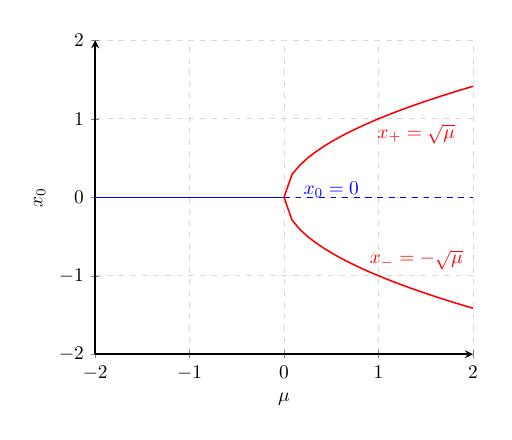
\begin{tikzpicture}[scale=0.7]
        \begin{axis}[
        ymin =-2, ymax=2, 
        xmin=-2, xmax=2, 
        xlabel = {$\mu$},
        ylabel = {$x_0$},
        grid = both,                % griglia
        grid style = {dashed, gray!30},
        axis lines = left,          % assi più puliti
        thick, % linee più spesse
    ]


    \addplot[color=blue, domain=-2:0]{0};
    \addplot[color=blue, dashed, domain=0:2]{0};

     \node at (axis cs:0.5, 0.1) [color=blue]{$x_0=0$};


    \addplot[color=red, domain=0:2]{x^(1/2)};
    \addplot[color=red, domain=0:2]{-x^(1/2)};

    \node at (axis cs:1.4, 0.8) [color=red]{$x_+=\sqrt{\mu}$};
    \node at (axis cs:1.4, -0.8) [color=red]{$x_-=-\sqrt{\mu}$};
    \end{axis}
    \end{tikzpicture}
    \end{center}

    Per la forma caratteristica del grafico, questa biforcazione è detta \emph{biforcazione a forchetta}. 
\end{example}

In effetti, non si tratta dell'unica biforcazione possibile. In generale, queste sono molto complicate ma si riducono a tre biforcazioni elementari, date da forchetta, trans-critica, e di Hopf. Vediamo due esempi per queste ultime: 

\begin{example}
    Un'esempio semplice di biforcazione trans-critica è data dall'eq., sempre in $\mathbb{R}^1$, data da 
    \begin{equation}
        \dot{x} = \mu x - x^2 = x(\mu -x)
    \end{equation}

    Chiaramente questa ha due punti fissi, dati da $x_0 =0, x_1 = \mu$. Ne possiamo studiare rapidamente la stabilità: $L = \mu - 2x$, così che si avrà: 

    \begin{enumerate}
        \item $x_0$ \\
        \begin{equation}
            L|_{x=0} = \mu = 
            \begin{cases}
                \text{stabile} \quad \mu <0 \\ \text{instabile} \quad \mu >0 
            \end{cases}
        \end{equation}
        \item $x_1$ \\
        \begin{equation}
            L|_{x=\mu} = -\mu = \begin{cases}
                \text{instabile} \quad \mu <0 \\ \text{stabile} \quad \mu >0 
            \end{cases}
        \end{equation}
    \end{enumerate}

    Otteniamo dunque il seguente grafico: 
    \begin{center}
    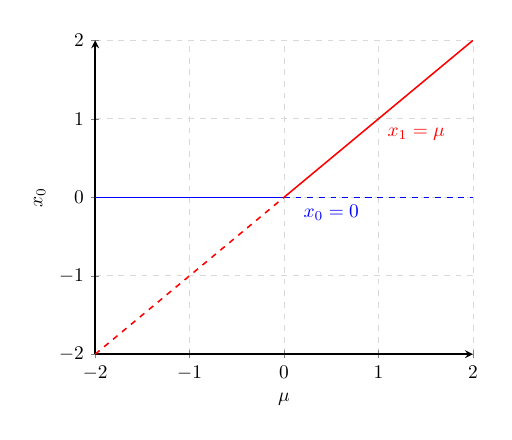
\begin{tikzpicture}[scale=0.7]
        \begin{axis}[
        ymin =-2, ymax=2, 
        xmin=-2, xmax=2, 
        xlabel = {$\mu$},
        ylabel = {$x_0$},
        grid = both,                % griglia
        grid style = {dashed, gray!30},
        axis lines = left,          % assi più puliti
        thick, % linee più spesse
    ]


    \addplot[color=blue, domain=-2:0]{0};
    \addplot[color=blue, dashed, domain=0:2]{0};

     \node at (axis cs:0.5, -0.2) [color=blue]{$x_0=0$};


    \addplot[color=red, , dashed, domain=-2:0]{x};
    \addplot[color=red, domain=0:2]{x};

    \node at (axis cs:1.4, 0.8) [color=red]{$x_1=\mu$};
    \end{axis}
    \end{tikzpicture}
    \end{center}

    Che è proprio il grafico tipico delle biforcazioni trans-critiche. 
\end{example}

\begin{example}
    Per vedere invece la biforcazione di Hopf, consideriamo il sistema dinamico in $\mathbb{R}^2$: 
    \begin{align}
        &\dot{x} = \mu x - y - (x^2 + y^2)x \\ &\dot{y}= \mu y + x -(x^2 + y^2)y 
    \end{align}

    Chiaramente l'origine è un punto fisso. Calcoliamo l'operatore $L$ nel punto: 
    \begin{equation}
        L|_{(0,0)} = \begin{pmatrix}
            \mu & -1 \\ 1 & \mu
        \end{pmatrix}
    \end{equation}
    Quali sono gli autovalori? Devo risolvere l'eq.
    \begin{equation}
        \text{det}(L - \lambda \mathbb{I}) = 0 
    \end{equation}
    ovvero devo risolvere l'eq. quadratica 
    \begin{equation}
        (\mu - \lambda)^2 +1 = 0 \xrightarrow{\tilde{u}= \mu - \lambda} \tilde{u} = \pm i \rightarrow \lambda = \mu \mp i \rightarrow \text{Re}(\lambda_i) = \mu 
    \end{equation}

    Questo mostra che l'origine è stabile se $\mu <0$, instabile se $\mu >0$. \\

    D'altra parte, potrei scrivere il sistema in coordinate polari: si otterebbe 
    \begin{align}
        &\dot{\theta} = 1 \\ &\dot{\rho} = (\mu - \rho^2)\rho
    \end{align}
    Dal quale si vede immediatamente che $\rho(t)\rightarrow \sqrt{\mu}$, ovvero la dinamica, per $\mu>0$, si riduce a moti periodici, sulla curva avente $\rho = \sqrt{\mu}$. Graficamente, potremmo rappresentare la biforcazione nel seguente modo: 

    \begin{center}
    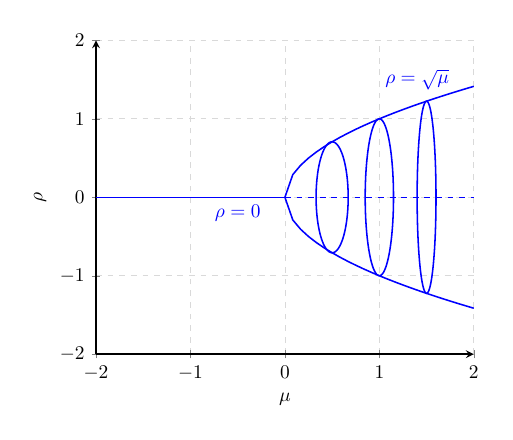
\begin{tikzpicture}[scale=0.7]
        \begin{axis}[
        ymin =-2, ymax=2, 
        xmin=-2, xmax=2, 
        xlabel = {$\mu$},
        ylabel = {$\rho$},
        grid = both,                % griglia
        grid style = {dashed, gray!30},
        axis lines = left,          % assi più puliti
        thick, % linee più spesse
    ]

    

    \addplot[color=blue, domain=-2:0]{0};
    \addplot[color=blue, dashed, domain=0:2]{0};

     \node at (axis cs:-0.5, -0.2) [color=blue]{$\rho=0$};

     \node at (axis cs:1.4, 1.5) [color=blue]{$\rho=\sqrt{\mu}$};

     \addplot[color=blue, domain=0:2]{x^(1/2)};
    \addplot[color=blue, domain=0:2]{-x^(1/2)};


    \addplot[
    domain=0:360,
    samples=100,
    thick,
    blue
    ] ({0.15*cos(x)+1},{1*sin(x)});


    \addplot[
    domain=0:360,
    samples=100,
    thick,
    blue
    ] ({0.17*cos(x)+0.5},{(2)^(-1/2)*sin(x)});

    \addplot[
    domain=0:360,
    samples=100,
    thick,
    blue
    ] ({0.1*cos(x)+1.5},{(3/2)^(1/2)*sin(x)});
    \end{axis}
    \end{tikzpicture}
    \end{center}

    Questa è proprio una biforcazione di Hopf: un punto fisso stabile che perde la sua stabilità, diventando orbite periodiche. \\
\end{example}

\subsection{La serie di Poincarè-Lindested}

Ora, vorremmo cercare di portare in un contesto astratto gli esempi che abbiamo visto. Considero ancora l'equazione 
\begin{equation}
    \dot{x} = \mu x- x^3
\end{equation}

e supponiamo di non conoscere le soluzioni stazionarie. Ci rendiamo conto che $\mu=0$ è un punto critico, e allora ci viene l'idea di studiare cosa succede per $|\mu| <<1$. Esprimiamo allora $x$ come una serie nelle potenze di $\mu$: 
\begin{equation}
    x = \sum_k c_k \mu^k
\end{equation}
La nostra equazione (per soluzioni stazionarie) diventa allora:  
\begin{equation}
    \mu \left(\sum_k c_k u^k \right) - \sum_{k, \ell, m} c_k c_\ell c_m u^{k+\ell+m} =0
\end{equation}

Ora possiamo risolvere per i coefficienti della serie, per ottenere l'espressione di $x$, richiedendo che i coefficienti di ciascuna delle potenze di $\mu$ si annulli. Così facendo otteniamo: 

\begin{align}
    &[\mu^0]: 0=0 \\ &[\mu^1]: 0=0 \\ &[\mu^2]: c_1=0 \\ &[\mu^3]: c_2 -c_1^3=0 \\ &[\mu^4]: c_3 -c_2c_1^2 - c_s^2c_1=0 \\ &...
\end{align}

Chiaramente l'unica soluzione del sistema è data da $c_i = 0, \quad \forall i$. Ingenuamente, penseremmo di concludere che non vi siano altre soluzioni stazionarie. Ma noi abbiamo già fatto il conto, ed abbiamo visto che le soluzioni $x_\pm = \pm \sqrt{\mu}$ sono delle soluzioni stazionarie al problema. Come mai non le abbiamo trovate? Ma certo, abbiamo espresso $x$ in termini di potenze "intere" di $\mu$, che chiramente non includono $\mu^{1/2}$. \\

Questo suggerisce che, se ho a che fare con dei polinomi, io debba piuttosto usare la \emph{serie di Poincarè-Lindested}: esprimo in serie di potenze sia $x$, sia $\mu$: se lo faccio per il nostro problema, ottengo, risparmiando i calcoli, 

\begin{align}
    &x = \sum_k c_k \epsilon^k \rightarrow x = c_1^2\epsilon^2 + 2c_2c_1\epsilon^3 + ...\\ &\mu = \sum_k a_k \epsilon^k  \rightarrow \mu = c_1\epsilon + c_2\epsilon^2 + ...
\end{align}

Dove $c_i$ sono parametri liberi. \\
In particolare, se prendiamo $c_i =0, \,  \forall i \geq 2$, ritroviamo proprio $x = \pm \sqrt{\mu}$. \\


\subsection{La riduzione di Lyapunov-Schmidt}
Consideriamo ora un'altra situazione: 
prendiamo il sistema dinamico

\begin{align}
    &\dot{x} = \mu x - xy^2 \\ &\dot{y} = x - y - x^2y
\end{align}

Come al solito, osservo che $(0,0)$ è un punto fisso $\forall \mu$, e calcolo 
\begin{equation}
    L|_{(0,0)} = \begin{pmatrix}
        \mu & 0 \\ 1 & -1
    \end{pmatrix}
\end{equation}

Gli autovalori della matrice sono dati da $\lambda_1 = -1, \lambda_2 = \mu$, così che $(0,0)$ è stabile per $\mu<0$, instabile se $\mu>0$. Quanto vale $L$ al punto critico? Troviamo subito che 

\begin{equation}
    L|_{(0,0)}(\mu=0) = L^* = \begin{pmatrix}
        0 &  0 \\ -1 & 1
    \end{pmatrix}
\end{equation}

Quali sono le proprietà di questa matrice? Cerchiamo il suo nucleo: 
\begin{equation}
    L^* \begin{pmatrix}
        x \\ y
    \end{pmatrix} = \begin{pmatrix}
        0 \\ x-y
    \end{pmatrix}
     = \begin{pmatrix}
         0 \\ 0 
     \end{pmatrix}
\end{equation}

Il che mostra che $\dim(\text{Ker}(L^*))=1$, che è sufficiente a mostrare anche che $\dim(\text{Ran}(L^*))=1$ (teorema di rango + nullità), e inoltre $\mathbb{R}^2 = \text{Ker}(L^*) \oplus \text{Ran}(L^*)$.  

Questo è importante perchè voglio cercare soluzioni stazionarie. D'altra parte, io posso anche cercare di risolvere il sistema non linearizzato, che semplicemente mi dice (dalla seconda equazione): 
\begin{equation}
    y = \frac{x}{(1+x^2)}
\end{equation}
e sostituendo nella prima 
\begin{equation}
    \mu x - x\frac{x^2}{(1+x^2)^2} = 0 
\end{equation}

Posso così scrivere $x(\mu)$, e dunque $y(x(\mu))$. \\


Vogliamo trarre una lezione generale da questo esempio. Questo da' un metodo, noto come \emph{decomposizione di Lyapunov-Schmidt}. Il problema è il seguente: suppongo di voler risolvere un'equazione del tipo 

\begin{equation}
    L(u) = F(u)
\end{equation}


Dove $L$ è un operatore, che dipende da un parametro $\mu$. Supponiamo che $\mu=0$ sia un punto critico, ed espandiamo $L$ in un intorno del punto critico: troveremo
\begin{equation}
    \left(L_0 + \sum_k \mu^kL_k \right)(u) = F(u) \rightarrow L_0 (u) = \left(F -\sum_k \mu^kL_k\right) (u) = G(u, \mu)
\end{equation}
Cosidero allora due proiettori, $P, Q$, t.c. 

\begin{align}
    &P: \mathbb{R}^n \rightarrow \text{Ker}(L_0)  \\
    & Q: \mathbb{R}^n \rightarrow \text{Ran}(L_0)
\end{align}

Osservo che posso allora sempre scrivere $u = w + v$, dove $v = (I-P)u, \, w = Pu$. In questo modo, scrivo 
\begin{equation}
    L_0(u) = L_0(v) = G(v, w,  \mu)
\end{equation}

Ora, questa equazione ha una soluzione solo se $G(w, v, \mu) \in \text{Ran}(L_0)$. Dunque, posso denotare $QG = \phi, \, (1-Q)G = \psi$, e la mia equazione è equivalente al sistema 

\[\begin{cases}
    L_0(v) = \phi(u, v, \mu) \\ \psi = 0 
\end{cases}\]

Ora osservo che, poichè nella prima equazione, $L_0$ ammette una preudo-inversa, il teorema della funzione implicita mi dice che da questa io posso sempre risolverla ed estrarre $w = w(v, \mu)$. A questo punto, l'unica equazione che mi rimane da risolvere è data da 

\begin{equation}
    0 = \phi(v, w(v, \mu), \mu) = \Theta(v, \mu)
\end{equation}

Questa è l'equazione più interessante, perchè mi lega gli elementi $v \in \text{Ker}(L_0)$, e il parametro $\mu$. Per questo motivo è detta \emph{equazione di biforcazione}. \\ Osserviamo che $L$ può essere uno strano operatore che agisce su uno spazio infinito-dimensiale (e.g. $L^2(\mathbb{C})$), ma finchè $\dim(\text{Ker}(L_0)) < + \infty$, allora l'equazione di biforcazione è finito-dimensionale. \\ 

Spesso, quando si usa la decomposizione LS, la si usa in combinazione con la serie di Poincarè-Lindested. Questo perchè il teorema della funzione imolicita garantisce che esista una funzione $w(v, \mu)$, ma non garantisce che possiamo calcolarla esplicitamente. Diamo dunque un'idea generale di cosa succede in questo caso, prima di fare un esempio esplicito: 

Dopo avere espresso $L$ in potenze di $\mu$, scriviamo 
\begin{equation}
    L_0(u) = G(u, \mu)
\end{equation}

Il metodo di Poincarè-Lindested prevede di espandere in serie $u, \mu$: 
\begin{align}
    u = \sum_k u_k \epsilon^k, \, \mu = \sum_k \mu_k \epsilon^k
\end{align}

Che implica una espansione in $G$: 
\begin{equation}
    G = \sum_k G_k (u, \mu)\epsilon^k
\end{equation}

L'eq. si frammenta nelle equazioni per le compomenti k-esime:
\begin{equation}
    L_0 (u_k) = G_k(u, \mu)
\end{equation}

Per $k=1$, questa è data semplicemente da \footnote{Questo perchè $G$ non ha nessuna parte lineare. Questo non lede alla generalità perchè se avesse una parte lineare potrei scrivere $G(u, \mu) = G_{lin}(u) + G'(u, \mu)$, e l'equazione diventerebbe $L_0' (u) = G'(u, \mu)$, dove $L_0' = L_0 - G_{lin}$}. 
\begin{equation}
    L_0(u_1) = 0  \rightarrow u_1 \in \text{Ker}(L_0)
\end{equation}

Ad ordini successivi, proietto sul range di $L_0$ ed il suo complementare: 
\[\begin{cases}
    L_0 (u_k) = Q(G_k) =: R_k \rightarrow u_k = L_0^*R_k\\ 
    (\mathbb{I}-Q)G_k =: \delta_k(u, \mu) = 0 
\end{cases}\]

Dove abbiamo indicato con $L_0^*$ la pseudoinversa di $L_0$ sul range. \\
Come al solito, la seconda equazione è quella interessante, perchè lega $u, \mu$. \\

Vediamo dunque un esempio: 

\begin{example}
    Si consideri il seguente sistema dinamico: 
    \[\begin{cases}
        \dot{x} = x - 2y -z^2 - xz \\ \dot{y} = 3x - 2y - 3z^3 - yz \\ \dot{z} = \mu z - z^3
    \end{cases}\]
    Cerchiamo soluzioni stazionarie: per prima cosa, notiamo che questo è equivalente all'equazione 
    \begin{equation}
        L_0(u) + \mu L_1(u_1) = F
    \end{equation}
    Dove 
    \begin{equation}
        L_0 = \begin{pmatrix}
            1 & -2 & 0 \\ 3 & -2 & 0 \\ 0 & 0 & 0 
        \end{pmatrix}
        , \quad 
        L_1 = \begin{pmatrix}
            0 & 0 & 0 \\ 0 & 0 & 0 \\ 0 & 0 & 1
        \end{pmatrix}, \quad 
        F = \begin{pmatrix}
            z^2 + xz \\ 3z^3 + yz \\ z^3
        \end{pmatrix}
    \end{equation}
    Ora sviluppo $u, \mu$ in serie: 
    \[\begin{cases}
        x = \sum_k \xi_k \epsilon^k \\ y = \sum_k \eta_k \epsilon^k \\ z = \sum_k \zeta_k \epsilon^k \\ \mu = \sum_k \mu_k \epsilon^k
    \end{cases}\]

    Come sempre succede, l'ordine 1 in $\epsilon$ è dato da 
    \begin{equation}
        L_0 (u_1) = 0 
    \end{equation}

    Dall'espressione di $L_0$ è chiaro che 
    \begin{equation}
        \text{Ker}(L_0) = \begin{pmatrix}
            0 \\ 0 \\ \zeta_1
        \end{pmatrix}, \zeta_1 \in \mathbb{R}
    \end{equation}

    Così che $\xi_1 = \eta_1 = 0$, mentre $\zeta_1$ rimane indeterminato, e per comodità denoteremo $w = \zeta_1$. \\
    Passiamo dunque all'ordine 2 in $\epsilon$: 

    \begin{equation}
        L_0(u_2) + \mu_1L_1(u_1) = F_2
    \end{equation}

    Dove $F_2$ è la parte quadratica in $\epsilon$ di $F$, data da 
    \begin{equation}
        F_2 = \begin{pmatrix}
            w^2 \\ 0 \\ 0
        \end{pmatrix}
    \end{equation}

    Definiamo allora 
    \begin{equation}
        \mathcal{N}_2 = F_2 - \mu_1L_1(u_1) = \begin{pmatrix}
            w^2 \\ 0 \\ -\mu w
        \end{pmatrix}
    \end{equation}

    Ancora una volta, l'eq. $L_0(u_2) = F_2$ ha soluzione solo se $F_2 \in \text{Ran}(L_0)$, il che vuol dire che dato $Q$ il proiettore sul range, dovrà valere 
    \[\begin{cases}
        (\mathbb{I}-Q)\mathcal{N}_2 = 0 \\ u_1 = L_o^*Q\mathcal{N}_2
    \end{cases}\]

    Poichè il range di $L_0$ è lo spazio $(x \quad y \quad 0)$ con $x, y, \in \mathbb{R}$, la prima equazione implica $\mu_1 = 0$. Poi posso calcolare 

    \begin{equation}
        L_0^* = \frac{1}{4}\begin{pmatrix}
            -2 & 2 \\ -3 & 1
        \end{pmatrix}
    \end{equation}

    Così che troverò
    \begin{equation}
        \begin{pmatrix}
            \xi_2 \\ \eta_2
        \end{pmatrix}
        = \frac{1}{4}\begin{pmatrix}
            -2 & 2 \\ -3 & 1
        \end{pmatrix}\begin{pmatrix}
            w^2 \\ 0
        \end{pmatrix}
    \end{equation}

    Svolgento la moltiplicazione, ottieniamo che $\xi_2 = -w^2/2$, $\eta_2 = -(3/4)w^2$. Essendoci ristretti sul range, non abbiamo condizioni su $\zeta_2$, che rimane indeterminato. Senza perdere generalità, possiamo porlo uguale a 0. Per riassumere, all'ordine 2 abbiamo trovato 
    \begin{equation}
        \mu_1 = 0, \quad \xi_2 = -\frac{w^2}{2}, \quad \eta_2 = -\frac{3w^2}{4}, \quad \zeta_2 = 0
    \end{equation}

    Passiamo allora all'ordine 3. L'eq. è data da 
    \begin{equation}
        L_0(u_3) + \mu_2L_1(u_1) = F_3
    \end{equation}

    Calcoliamo allora 
    \begin{equation}
        \mathcal{N}_3 = F_3 - \mu_2L_1(u_1) =\begin{pmatrix}
            \zeta_1\xi_2 + \xi_1\zeta_2 \\ 3\zeta_1^3 + \eta_q\zeta_2 + \zeta_1\eta_2 \\ \zeta_1^3 - \mu_2\zeta_1
        \end{pmatrix} = \begin{pmatrix}
            -w^3/2 \\ 3w^3 -(3/4)w^3\\ w^3 -\mu_2w
        \end{pmatrix}
    \end{equation}

    La proiezione lungo il complementare del range deve essere nulla, così che varrà 
    \begin{equation}
        w(w^2 - \mu_2) = 0 \rightarrow \mu_2 = w^2
    \end{equation}
    Invece 
    \begin{equation}
        \begin{pmatrix}
            \xi_3 \\ \eta_3 
        \end{pmatrix} = \frac{1}{4}\begin{pmatrix}
            -2 & 2 \\ -3 & 1
        \end{pmatrix}\begin{pmatrix}
            -\frac{1}{2}w^3 \\ -\frac{9}{4}w^3 
        \end{pmatrix}
        = \frac{w^3}{4}\begin{pmatrix}
            7/2 \\ 15/4
        \end{pmatrix}
    \end{equation}
    Fermandoci all'ordine 3, abbiamo trovato che 
    \begin{equation}
        u = \begin{pmatrix}
            x \\ y \\ z 
        \end{pmatrix}
        = \begin{pmatrix}
            -(1/2)w^2\epsilon^2 + (7/8)w^3\epsilon^3+ ...\\ -(3/4)w^2\epsilon^2 + (15/16)w^3\epsilon^3 + .. \\ w\epsilon 
        \end{pmatrix}
    \end{equation}

    Da cui ci accorgiamo che il vero parametro in cui vi è l'espansione non è $\epsilon$ ma il prodotto $w\epsilon$. Ponendo $w =1$, troviamo infine 
    \begin{align}
        u 
        = \begin{pmatrix}
            -(1/2)\epsilon^2 + (7/8)\epsilon^3+ ...\\ -(3/4)\epsilon^2 + (15/16)\epsilon^3 + .. \\ \epsilon 
        \end{pmatrix}, \quad \mu = \epsilon^2 + ...
    \end{align}
\end{example}

Questo era un esempio finito-dimensionale, ma la teoria è di fatto valida se gli operatori sono operatori di Fredholm, cioè in particolare se il nucleo dell'operatore ha dimensione finita. Vediamo allora un esempio di questo tipo: \\

\ex{}{
    Consideriamo l'equazione differenziale alle derivate parziali 
    \begin{equation}
        \frac{\partial u}{\partial t} = \frac{\partial^2 u}{\partial x^2} + \mu u - u^2
    \end{equation}
    Dove $u = u(x,t)$, e valgono le condizioni al contorno di Dirichlet, $u(0,t) = u(L, t) = 0$. Denoteremo $\mathcal{B}$ tale spazio funzionale. \\
    Questo ci permette di scegliere di scrivere le nostre funzioni nella base dei seni: 
    \begin{equation}
        u(x, t) = \sum_k \alpha_k \sin{\left(\frac{k\pi x}{L} \right)}
    \end{equation}

    Se cerchiamo soluzioni stazionarie, allora questo è equivalente a risolvere il problema 
    \begin{equation}
        G(u, \mu) = 0, \quad G = \left(\frac{\partial^2}{\partial x^2} + \mu\right)u - u^2
    \end{equation}

    Per prima cosa, considero lo spettro della parte lineare di $G$, data da 
    \begin{equation}
        L =\left(\frac{\partial^2}{\partial x^2} + \mu\right)
    \end{equation}

    Osservo in particolare che questo operatore è diagonale nella base che ho scelto, ed ha spettro dato da 
    \begin{equation}
        L_0\ket{k} = (-k^2 + \mu)\ket{k}
    \end{equation}

    Se questi sono tutti negativi (cioè vale $k^2 > \mu$), la dinamica è stabile. D'altra parte, $k = \pm 1, \pm 2, ..$ così che il punto $\mu_0 = 1$ è un punto critico. Per prima cosa, osservo che posso scrivere 
    \begin{equation}
        L = L_0 + (\mu- \mu_0)L_1, \quad L_0 = \left(\frac{\partial^2}{\partial x^2} + \mu_0\right), \quad L_1 = 1
    \end{equation}

    Così che l'equazione per le soluzioni stazionarie sia data da 
    \begin{equation}
        L_0(u) + (\mu- \mu_0)L_1(u) = F(u), \quad F(u) = u^2
    \end{equation}

    Ora applichiamo il metodo di Poincarè-Lingested, che ricordiamo prevede di esprimere in serie $u, \mu$ in termini di potenze di un parametro $\epsilon$. \\

    Scriviamo allora 
    \begin{align}
        &\mu = \mu_0 + \sum_k \mu_k\epsilon^k \\
        & u = \phi + \psi = \sum_k \phi_k\epsilon^k + \sum_k\psi_k\epsilon^k
    \end{align}

Dove abbiamo già convenientemente diviso $u$ in $\phi \in \text{Ker}(L_0)$, $\psi \in (\text{Ker}(L_0))^{\perp}$. Si noti, inoltre, che anche i coefficenti $\psi_k, \phi_k$ sono naturalmente delle funzioni nello spazio funzionale delle nostre soluzioni, ed in particolare saranno anche esse scritte nella base dei seni (cioè varrà $\psi_k = \sum_j \tilde{\psi}_{jk}\ket{j}$). Come sempre succede, al primo ordine l'equazione ci dice 
\begin{equation}
    L_0(u_1) = L_0(\phi_1 + \psi_1) = L_0(\psi_1) = 0  
\end{equation}

Il che ha come unica soluzione $\psi_1 = 0$, mentre $\phi_1$ rimane un indeterminato membro del nucleo di $L_0$. In effetti, il kernel di $L_0$ è dato da 
\begin{equation}
    L_0\ket{k} = (-k^2 + \mu_0)\ket{k} = 0 \rightarrow k^2 = \mu_0 = 1 \rightarrow \text{Ker}(L_0) = \varphi \ket{1}, \varphi \in \mathbb{R}
\end{equation}

Senza ledere alla generalità in questo caso consideriamo $\varphi = 1$, così che il risultato dell'equazione al primo ordine è dato da 
\begin{equation}
    \psi_1 = 0, \quad \phi_1 = \ket{1}
\end{equation}

Passiamo al secondo ordine. L'equazione è data da 
\begin{equation}
    L_0(u_2) = -(\mu_1 - \mu_0)L_1(u_1) + (u_1)^2
\end{equation}
Ovvero 
\begin{equation}
    \ket{L_0(\psi_2)} = -(\mu_1-\mu_0)\ket{1} + (\ket{1})^2
\end{equation}

Consideriamo ora la proiezione sul nucleo
\begin{equation}
    P : \mathcal{B} \rightarrow \text{Ker}(L_0), \quad P = \ket{1}\bra{1}
\end{equation}

Per comodità indichiamo la funzione $\ket{1}^2 := \ket{1^2}$. Proiettando l'equazione troviamo 
\begin{equation}
    \bra{1}\ket{L_0\psi_2}\ket{1} = -(\mu_1-1)\ket{1} + \braket{1|1^2}\ket{1}
\end{equation}

Poichè $L_0$ è un operatore diagonale, esisterà $\lambda$ t.c. $\braket{L_0|\psi_2} = \lambda \braket{1|\psi_2} = 0$. Trovo allora 
\begin{equation}
    (\mu_1 - \mu_0 - \braket{1|1^2})\ket{1} = 0
\end{equation}
Che è un'equazione per $\mu_1$: 
\begin{equation}
    \mu_1 = \mu_0 + \braket{1|1^2} = 1 + \braket{1|1^2}
\end{equation}
facilmente risolvibile ricordando il prodotto scalare
\begin{equation}
    \mu_1 = 1 + \frac{2}{L}\int_0^{L}\sin^3\left(\frac{\pi x}{L} \right)dx
\end{equation}

Ora possiamo passare all'equazione sul complementare del nucleo: 

\begin{equation}
    L_0(\psi_2) = (1 - \ket{1}\bra{1})\ket{1^2} = \ket{1^2} - \braket{1|1^2}\ket{1}
\end{equation}

L'equazione ha certamente soluzione. Possiamo scrivere 
\begin{equation}
    \psi_2 = \sum_k \beta^{(2)}_k \ket{k} \rightarrow L_0\psi_2 = - \sum_k \beta^{(2)}_k k^2\ket{k}
\end{equation}

Così che valga 
\begin{equation}
    \sum_k \beta^{(2)}_k k^2\ket{k} + \ket{1^2} - \braket{1|1^2}\ket{1} = 0
\end{equation}

Che è un'equazione risolvibile per i coefficienti $\beta^{(2)}_k$, una volta che si è scritto 
\begin{equation}
    \ket{1^2} = \sum_k \eta_k \ket{k}
\end{equation}
Con i coefficienti $\eta_k$ dati da 
\begin{equation}
    \eta_k = \braket{k|1^2} = \frac{2}{L}\int_0^L \sin^2\left(\frac{\pi x}{L} \right)\sin{\left(\frac{k\pi x}{L} \right)}
\end{equation}
}

\subsection{Un'altra idea di Poincarè}


Abbiamo visto come sia determinate sapere risolvere le equazioni del tipo 
\begin{align}
    \dot{x} = f(x)
\end{align}

Dove \(f(x)\) è un campo vettoriale, ovvero \(f: \mathbb{R}^n \rightarrow \mathbb{R}^n\). \\

Ora, l'equazione può essere certamente integrata se esiste una qualche trasformazione \(y = y(x)\), sotto la quale l'equazione diventi 

\begin{align}
    \dot{y} = A y
\end{align}

Con \(A\) un operatore lineare su \(\mathbb{R}^n\) (cioè una matrice). D'altra parte, Poincarè viveva in un epoca dove si pensava che tutti i sistemi fossero integrabili, e dunque voleva cercare una forma generale di trasformazione di coordiante, che permettesse di scrivere l'equazione  lineare. \\

Per fare questo, espando \(f(x)\) in funzioni omogenee di grado \(k\): 
\begin{align}
    \dot{x} = A x + \sum_{k=2}^{+\infty} F_k(x), \quad F_k(\alpha x) = \alpha^k F_k(x), \, \forall k
\end{align}

Poincarè allora prese una trasformazione del tipo \(x = y + h_m(y)\), con \(h_m\) una funzione omogenea di grado \(m\), che rende l'equazione

\begin{align}
    \dot{y}^i + \frac{\partial h^i_{(m)}}{\partial y^j}\dot{y}^j = A^i_j y^j + A^i_j h^j + \sum_k F_{(k)}(y + h(y))
\end{align}


\chapter{Teorie di gauge}

\section{Aspetti di topologia e geometria differenziale}

Le teorie di gauge sono un pezzo fondamentale della fisica teorica. Il modello standard, ovvero la teoria più precisa esistente delle particelle elementari, è una teoria di gauge. Descrive insieme forza elettromagnetica, debole e forte. D'altra parte, queste teorie hanno anche attirato l'interesse dei matematici, che hanno riconosciuto un profondo legame delle teorie con argomenti avanzati di geometria differenziale e topologia. Per comprendere anche il punto di vista matematico, allora, è prima necessario dare qualche definzione ed esempio degli strumenti che ci verranno utili in seguito. \\

\subsection{Omologia}

Cominciamo a dire che cosa è l'\emph{omologia}: 

\dfn{Omologia}{

    L'omoologia è la branca della topologia che si occupa di \emph{distinguere} varietà topologicamente diverse. 
}

Cominciamo allora considerando una varietà \(M\) liscia e connessa. La sua p-catena è definita come la somma \emph{formale}

\begin{align}
    a_p = \sum_i c_iN_i 
\end{align}

Dove in particolare

\begin{enumerate}
    \item \(N_i\) : \\
    sono le sottovarietà di \(M\) lisce e orientate, t.c. \(\dim (N_i)=p\)
    \item \(c_i\) : \\
    sono degli opportuni coefficenti, che possono essere in \(\mathbb{R}, \mathbb{C}, \mathbb{Z}, \mathbb{Z}_2 = \left\{0, 1 \right\}\)
\end{enumerate}

A partire da \(a_p\) si definisce la (p-1)-catena, data da 

\begin{align}
    \partial a_p = \sum_i c_i \partial N_i
\end{align}

dove con il simbolo \(\partial\) indichiamo l'operazione di prendere il bordo. Molto importante è il set dei cicli: 

\begin{align}
    Z_p := \left\{a_p : \partial a_p = \emptyset \right\}
\end{align}

che è dunque il set delle p-catene senza bordo. Definiamo inoltre il set 

\begin{align}
    B_p = \left\{\partial a_{p+1}\right\}
\end{align}

ovvero il set delle p-catene che si possono scrivere come il bordo di (p+1)-catene. Ricordando allora che vale \(\partial \partial a_p = \emptyset, \, \forall p\), è chiaro che vale \(B_p \subset Z_p\). Possiamo allora finalmente definire 

\begin{align}
    H_p = Z_p \setminus B_p
\end{align}

Tipicamente si indica \(H_p(M, G)\), dove \(M\) è la varietà e \(G = \left\{\mathbb{R}, \mathbb{C}, \mathbb{Z}, \text{ecc.} \right\}\). Valgono allora le seguenti proprietà: 

\begin{enumerate}
    \item \(H_p (M, G) = 0, \quad p> \dim M\) 
    \item Se \(M\) è connesso, \(H_0(M, G) = G\) 
    \item Se \(M\) è orientato, \(H_n(M, G) = G\)
\end{enumerate}

Tipicamente la più importante è la \(H_p(M, \mathbb{Z})\), poiché un teorema, detto dei coefficienti universali, da come trovare l'omologia rispetto agli altri campi a partire da questo. 

\subsection{Varietà complesse}

Diamo ora una descrizione qualitativa delle proprietà fondamentali delle varietà complesse, dando qualche esempio notevole. \\

Cominciamo subito descrivendo la sfera di Riemann: 

\ex{Sfera di Riemann}{

    La \(S^2\), che è una varietà bidimensionale, può esserre pensata come una varietà complessa 1-dimensionale. Le coordinate locali sono date dalla solita proiezione stereografica. Prendi due aperti che coprano la due-sfera, dati da 

    \begin{align}
        U = S^2 \setminus \left\{(0, 0, 1) = N\right\}, \quad \tilde{U} = S^2 \setminus \left\{(0, 0, -1) = S\right\}
    \end{align}

    Se \((u_1, u_2, u_3) \in S^2\), i.e. vale \(u_1^2 + u_2^2 + u_3^2 = 1\), allora secondo le regole della proiezione stereografica, le coordinate locali sulle due carte sono date da 

    \begin{align}
        &\lambda = \frac{u_1 + iu_2}{1 - u_3}, \quad \text{in } U\\
        &\tilde{\lambda} = \frac{u_1 - iu_2}{u_3 -1} \quad \text{in } \tilde{U}
    \end{align}

    L'unica cosa che ci rimane da controllare è che nella regione \(U \cap \tilde{U}\) la mappa fra le coordinate locali sia olomorfa. Osserviamo allora che 

    \begin{align}
        \lambda &=  \frac{u_1 + iu_2}{1 - u_3} =\frac{(u_1 + iu_2)(u_1 - iu_2)}{(1 - u_3)(u_1 - iu_2)} \\
        &= \frac{u_1^2 + u_2^2}{(1 - u_3)(u_1 - iu_2)} = \frac{1 - u_3^2}{(1 - u_3)(u_1 - iu_2)} = \frac{1 + u_3}{u_1 - iu_2} = (\tilde{\lambda})^{-1}  
    \end{align}

    dunque anche quest'ultima condizione è soddisfatta. 

}

Un'altro esempio che ci verrà utile è lo spazio dei rapporti: 

\ex{\(\mathbb{CP}^n\)}{

    Una varietà n-dimensionale che si può costruire da \(\mathbb{C}^{n+1}\), è lo \emph{spazio proiettivo complesso}: in pratica, si tratta dello spazio complesso \((n+1)\)-dimensionale, quozientato dalla relazione di equivalenza 

    \begin{align}
        (Z_0, \ldots, Z_n) \equiv (cZ_0, \ldots, cZ_n), \quad \forall c \in \mathbb{C}^* = \mathbb{C} \setminus 0 
    \end{align}

    Una possibile parametrizzazione è la seguente: sia \(U_\alpha= \mathbb{C}^{n+1} \setminus Z_\alpha = 0\). \\
    
    Su ciascuna di queste carte, definiamo \(z^a, \, a = \left\{(1, \ldots, n)\right\}\), data da 

    \begin{align}
        z^i = Z^i / Z^{\alpha}
    \end{align}

    dove nel lato destro dell'equazione, \(i \in (1, \ldots, \alpha -1, \alpha +1, \ldots, n+1)\). 
}

Come si fa a dire che due varietà complesse sono isomorfe? Prima di tutto, dobbiamo capire il significato di una funzione \(f: \mathcal{M} \rightarrow \mathcal{M}'\), se \(\mathcal{M}, \mathcal{M}'\) sono due varietà complesse. \\

Si ha allora la seguente definizione: 

\dfn{Funzione olomorfa fra varietà complesse}{

    Siano \(\mathcal{M}, \mathcal{M}'\) due varietà complesse, di dimensione \(n, n'\). Le loro carte sono funzioni \(\phi_\alpha: U_\alpha \rightarrow \mathbb{C}^n\), e \(\phi'_\beta : U_\beta \rightarrow \mathbb{C}^{n'}\). Si dice allora che una funzione \(f: \mathcal{M} \rightarrow \mathcal{M}'\) è olomorfa, s.se \(\forall \phi_\alpha, \phi_\beta\) la funzione \(\phi'_\beta * f * \phi^{-1}_\alpha\) è olomorfa. 
}

Nota che la definizione ha senso, poichè \(\phi^{-1}_\alpha : \mathbb{C}^n \rightarrow U_\alpha\), \(f: U_\alpha \rightarrow U_\beta\), ed infine \(\phi_\beta : U_\beta \rightarrow \mathbb{C}^{n'}\). Dunque le funzioni risultanti sono tutte funzioni tra i due spazi complessi.  

Possiamo allora dire quando due varietà complesse sono isomorfe: 

\dfn{Varietà isomorfe}{

    Due varietà complesse sono isomorfe se sono diffeomorfe, tramite una funzione \(f\) che è bi-olomorfa, i.e. sono olomorfe sia \(f\), sia \(f^{-1}\). 
}

\nt{
    Alla luce delle definizioni che abbiamo dato, possiamo dire 

    \begin{align}
        \mathbb{CP}^1 \simeq S^2
    \end{align}

    Dove la \(S^2\) è intesa come varietà complessa, i.e. la sfera di Riemann. Molte volte per questo fatto si indica proprio con \(\mathbb{CP}^1\) la sfera di Riemann. \\ 

    Mostriamo che vale l'isomorfismo: per prima cosa, ricordiamo cosa sono in questo caso le carte, e gli aperti dove sono definiti: 

    \begin{enumerate}
        \item \(S^2\): la due sfera può essere coperta da due aperti, \(U = S^2 \setminus N, \, \tilde{U} = S^2 \setminus S\). Le carte locali su queste sono date da \(\lambda = \frac{u_1 + iu_2}{1-u_3}, \, \tilde{\lambda} = \frac{u_1 -iu_2}{u_3 -1}\). 
        \item \(\mathbb{CP}^1\): se \(n=1\), prendiamo i seguenti aperti che coprono \(\mathbb{C}^2\): \(U = \mathbb{C}^2 \setminus \left\{Z^1 =0 \right\}, \tilde{U} = \mathbb{C}^2 \setminus \left\{Z^2 =0 \right\}\), e su queste le carte \(\xi = \frac{Z^2}{Z^1}, \, \tilde{\xi} = \frac{Z^1}{Z^2} \). 
    \end{enumerate}

    Ora consideriamo la semplice mappa (proiezione stereografica) \(f: (u_1, u_2, u_3) \in S^2 \rightarrow [u_1 + iu_2, 1 - u_3] \in \mathbb{C}^2\): questa realizza l'isomorfismo, perchè è diffeomorfa, ed inoltre consideriamo 

    \begin{align}
        \xi * f * (\lambda)^{-1} = \, ? 
    \end{align}

    Poichè \(\lambda: U \rightarrow \mathbb{C}\), allora avremo che l'inversa va dalla \(S^2\) (senza considerare il polo nord), nello spazio complesso uno-dimensionale. 
}















































\subsection{Varietà Riemanniane}

Si dice varietà Riemanniana la coppia  \(M, g\), dove \(M\) è una varietà e \(g\) una metrica. La distanza infinitesima tra due punti è data allora da 

\begin{align}
    ds^2 = g_{\mu\nu}dx^{\mu}dx^{\nu}
\end{align}

esempi semplici sono lo spazio euclideo, con metrica \(g_{\mu\nu} = \delta_{\mu\nu}\), oppure lo spazio di Minkowski, con \(g_{\mu\nu} = \text{diag}(-, +, \ldots, +)\).  \\

Più in generale, vale che \(g_{\mu\nu} = g_{\mu\nu}(x)\). Si può allora scrivere 

\begin{align}
    g_{\mu\nu} = \eta_{ab}e^a_\mu e^b_\nu
\end{align}

dove invece \(\eta_{ab}\) è una metrica piatta, i.e. \(\partial_\mu \eta_{ab} =0\). \\

Le "inverse" di \(e^a_\mu\) sono date da 

\begin{align}
    E^{\mu}_{\, a} = g^{\mu\nu}\eta_{ab}e^b_\nu
\end{align}

infatti vediamo facilmente che 

\begin{align}
    E^{\mu}_{\, a}e^b_\mu = g^{\mu\nu}\eta_{ac}e^c_\nu e^b_\mu = g^{\mu\nu}\eta_{ac}e^c_\nu e^a_\mu \delta^b_a = g^{\mu\nu}g_{\mu\nu}\delta^b_a = \delta^b_a
\end{align}

Possiamo allora interpretare le \(e^a_\mu\) come una trasformazione delle coordinate \(dx^\mu\) di \(T^*(M)\). Questo è il punto di partenza della formulazione di Cartan delle varietà rimanniane in termini di forme differenziali. \\

Consideriamo allora la 1-forma connessione data da \(\omega^b_a\) \footnote{Per ora, prendiamo una connesione arbitraria. In generale, la connesione non è univocamente determinata data la struttura di varietà riemanniana. Vedremo tra poco che se invece facciamo alcune ipotesi allora la connesione assume una forma univoca che determineremo}. Chiamiamo \(e^a = e^a_\mu dx^\mu\). La 2-forma \emph{torsione} si definisce come 


\begin{align}
    T^a = de^a + d\omega^a_b \wedge e^b
\end{align}

e la 2-forma \emph{curvatura} è invece data da 

\begin{align}
    R^a_{\,\, b} = dw^a_{\,\, b} + w^a_{\,\, c} \wedge \omega^c_{\,\, b}
\end{align}

Queste due equazioni sono note come \emph{formule di struttura di Cartan}. Le loro derivate esterne sono le equazioni di \emph{consistenza} e l'\emph{identità di Bianchi}, e sono date rispettivamente da 

\begin{align}
    &dT^a + \omega^a_b T^b = R^a_b \wedge e^b \\
    &dR^a_{\,\, b} -R^a_{\, \, c}\wedge \omega^c_b + \omega^a_c \wedge R^c_b= 0 
\end{align}

Ora definiamo la derivata covariante che agisce su una p-forma \(V^a_b\), data da 

\begin{align}
    D V^a_b = dV^a_b + w^a_c \wedge V^c_b - (-)^p V^a_c \wedge w^c_b  
\end{align}

Ad esempio, l'identità di bianchi è data da 

\begin{align}
    D R^a_b = 0
\end{align}

Ora, questa è comoda perchè se considero ora una rotazione ortogonale della mia base ortonormale

\begin{align}
    e'_a = \Phi^a_b e^b
\end{align}

allora la derivata convariante di qualsiasi p-forma si trasforma anche lei come 

\begin{align}
    (DV)'^a_b = \Phi^a_c (DV)^c_d (\Phi^-1)^d_b
\end{align}

Chiaramente, la formulazione di Cartan in termini delle forme differenziali è equivalente alla formulazione tensoriale classica della geometria riemanniana. \\

In particolare, vediamo come sono legate le quantità fondamentali come la curvatura, la connessione e la torsione: inanzitutto, essendo le prime due 2-forme possiamo scriverle come 

\begin{align}
    &T^a = \frac{1}{2}T^a_{bc} \, e^b \wedge e^c = \frac{1}{2}T^a_{\mu\nu}dx^{\mu}\wedge dx^{\nu}\\
    &R^a_b = \frac{1}{2}R^a_{bcd} \, e^c \wedge e^d = \frac{1}{2}R^a_{b\mu\nu} dx^{\mu}\wedge dx^{\nu}
\end{align}

A questo punto, le vecchie componenti dei tensori si ottengono semplicemente usando \(E^a_\mu\), in particolare si ha che 

\begin{align}
    &R^\alpha_{\beta\mu\nu} = E^\alpha_a e^b_\beta R^a_{b\mu\nu} \\
    & T^\alpha_{\mu\nu} = E^{\alpha}_aT^a_{\mu\nu}
\end{align}

Per la connessione, la faccenda è leggermente più complicata. Tipicamente, quando si fa il calcolo tensoriale, si dice che le connessioni sono i \emph{simboli di Cristoffel}, che si ottengono imponendo che la derivata covariante della metrica sia nulla, e che la torsione sia nulla. In questo modo, si scrive che 

\begin{align}
    \Gamma^\mu_{\alpha \beta} = \frac{1}{2}g^{\mu\nu}\left\{\partial_\alpha g_{\nu\beta} + \partial_\beta g_{\nu\alpha} - \partial_\nu g_{\alpha\beta}\right\}
\end{align}

Similmente, nel metodo di Cartan si impone che valga \(\omega_{ab} = -\omega_{ba}\), ed inoltre che valga \(T^a = 0\). Con queste condizioni i coefficenti \(\omega^a_{b\mu}\) sono univocamente determinati e sono legati ai simboli di Cristoffel da 

\begin{align}
    \omega^a_{b\mu} = -E^\nu_b (\partial_\mu e^a_\nu - \Gamma^\lambda_{\mu\nu}e^a_{\lambda})
\end{align}


\subsection{I fibrati}

Molti concetti in fisica possono essere compresi in termini della geometria dei fibrati. Ad esempio, la teoria dell'elettromagnetismo o le teorie di Yang-Mills sono teorie di connessioni sul fibrato principale, con fibra data dal gruppo di gauge \(G\). Anche la teoria della gravitazione di Einstein centra con le connessioni di Levi-Civita sul fibrato delle basi dello spazio-tempo. \\

Ci rendiamo conto che è quindi opportuno cercare di comprendere cosa sono i fibrati, le loro proprietà, e vederne qualche esempio. Questo ci tornerà particolarmente utile quando vorremo considerare dal punto di vista matematico le teorie di gauge. \\

Cominciamo trattando l'argomento in modo non troppo formale. Consideriamo inanzitutto una varietà \(M\), ed una varietà \(F\). Queste varietà sono rispettivamente dette \emph{spazio base} e \emph{fibra}. Chiamiamo fibratu su \(M\) di fibra \(F\), una varietà \(E\), che è localmente il prodotto diretto di \(M, F\). 
Questo vuol dire che immaginiamo che \(M\) sia coperto da un'atlante \(U\) di carte \(U_i\), allora \(E\) è topologicamente descritto in ogni \(U_i\) dal prodotto diretto

\begin{align}
    U_i \times F 
\end{align}

Ad esempio, osserviamo la figura:

\begin{center}
    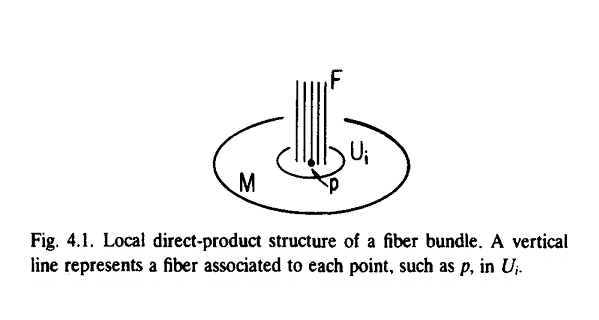
\includegraphics[scale=0.7]{fiberbundel.png}
\end{center}

Chiaramente, questo dice poco o niente sulla topologia globale del fibrato \(E\). Per superare questa difficoltà, dobbiamo aggiungere un set di \emph{funzioni di transizione} \(\left\{\phi_{ij}\right\}\), che ci dicono come la fibra si adegua nell'intersezione \(U_i \cap U_j\). Nello specifico, diciamo che 

\begin{align}
    \phi_{ij} : F_{U_i} \rightarrow F_{U_j}, \quad U_i \cap U_j
\end{align}

In generale, dunque, sebbene la topologia locale del fibrato sia banale, la topologia globale può essere complicata, e dipende dalle funzioni di transizione. Per questo motivo, spesso in letteratura matematica si dice che il fibrato è un \emph{twisted product}. \\

\ex{Il nastro di Mobius}{
    Un caso semplice di un fibrato non avente una topologia banale è il nastro di Mobius. \\

    Costruiamo il nostro fibrato nel seguente modo: come spazio di base scegliamo \(S^1\). Per prima cosa dobbiamo prendere un atlante che lo copra, e noi prendiamo 

    \begin{align}
        U = \left\{U_+, U_- \right\}, \quad &U_+ = \left\{\theta: -\eps < \theta < \pi + \eps\right\} \\
        &U_- = \left\{\theta: \pi -\eps < \theta < 2\pi + \eps\right\}
    \end{align}

    Ora dobbiamo scegliere la nostra fibra, che prendiamo essere l'intervallo dell'asse reale \([-1, 1]\). Il fibrato è a questo punto descritto da 

    \begin{enumerate}
        \item \(U_+ \times F\), con coordinate \(\theta, t_+\)
        \item \(U_- \times F\), con coordinate \(\theta, t_-\)
        \item le regole di transizione, che dobbiamo ancora decidere, che legano \(t_+, t_-\) in \(U_+ \cap U_-\). 
    \end{enumerate}


    Prendiamo allora che: 
    \begin{align}
        &\text{RI} = \left\{\theta \in (-\eps, \eps)\right\} \rightarrow t_+ = t_- \\
        &\text{RII} = \left\{\theta \in (\pi - \eps, \pi + \eps) \right\} \rightarrow t_+ = t_-
    \end{align}


    In particolare, la seconda mappa di transizione fa "girare" la striscia, e rende la topologia globale del fibrato non banale. La figura aiuta a visualizzare quello che abbiamo fatto: 

    \begin{center}
        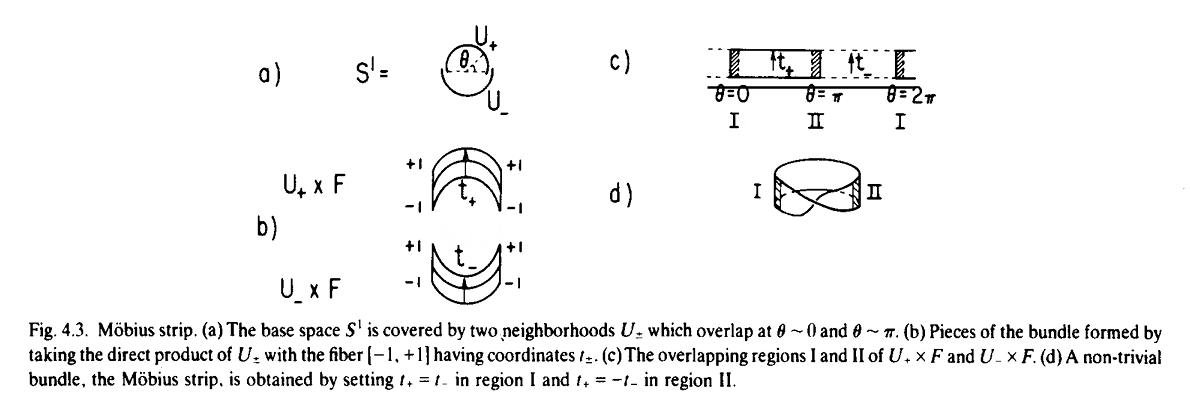
\includegraphics[scale= 0.5]{mobius.png}
    \end{center}
}

Chiaramente, se tutte le regole di transizione sono banali, ovvero se soni tutte l'identità, allora la topologia globale del fibrato è data da 

\begin{align}
    E = M \times F
\end{align}

questo tipo di fibrati sono detti \emph{fibrati banali}. Chiaramente, se avessimo preso l'identità anche nella seconda regione nell'esempio precedente, allora avremmo trovato che il fibrato era semplicemente un cilindro, \(S^1 \times [-1, 1]\). Un teorema assicura che ogni fibrato con spazio di base contraibile (cioè che è omotopicamente equivalente ad un punto), è banale. Questo è un teorema molto importante, perchè ci dice che fibrati non banali possono essere realizzati solo a partire da spazi di base non banali, ovvero \emph{non} contraibili (quindi non un set aperto di \(\mathbb{R}^n\), per esempio.) \\

Un aspetto importante di un fibrato sono le sue \emph{sezioni}: una sezione \(s\) di un fibrato \(E\) è una regola che assegna un punto \(s(x)\) sulla fibra, ad ogni punto \(x\) della varietà di base \(M\). Una sezione si dice locale se è definita solo un sottoinsieme dello spazio di base \(M\). In particolare, possiamo sempre definire delle sezioni locali sugli spazi \(U_i \times F\), ma in generale l'esistenza di sezioni globali dipende dalla topologia globale del fibrato. Esistono fibrati che non hanno sezioni globali. \\

Avendo discusso un po' euristicamente dei fibrati, possiamo ora essere più rigorosi: in particolare, una definizione più precisa dei fibrati richiede che sia introdotta una \emph{mappa di proiezione} \(\pi: E \rightarrow M\), che proietta il fibrato sullo spazio di base, di fatto riducendo la fibra ad un punto. \\

Sia \(x \in M\): diciamo che \(\pi^{-1}(x) \in E\) è la \emph{fibra su x}. Indicheremo spesso anche \(\pi^{-1}(U_i)\) il sottoinsieme del fibrato che viene proiettato su \(U_i\). Siamo pronti a dare la definizione: 

\dfn{Fibrato}{
    Un fibrato \(E\) con fibra \(F\) sulla varietà di base \(M\) è uno spazio topologico, assieme ad una proiezione \(\pi: E \rightarrow M\), che soddisfa la seguente condizione: \\
    Per ogni punto \(x \in M\), esiste un intorno \(U_i\) di \(x\) e un isomorfismo \(\phi_i\) che mappa \(U_i \times F\) in \(\pi^{-1}(U_i) \subset E\). Denotando con \(x, f\) un punto in \(U_i \times F\), richiediamo che \(\pi (\phi_i (x, f)) = x\). 
}


Con questa definizione formale, le funzioni di transizione sono date da

\begin{align}
    \phi_{ij} = \phi_i^{-1}\phi_j, \quad U_i \cap U_j
\end{align}

Chiaramente, poiché \(\phi: U_i \times F \rightarrow \pi^{-1}(U_i)\), questo vuol dire che per fissato \(x \in U_i \cap U_j \subset M\), le funzioni di transizione sono mappe dalla fibra \(F\) su se stessa. Richiediamo che le funzioni di transizione sono degli elementi di un gruppo \(G\) di trasformazioni sulla fibra. Il gruppo \(G\) è detto \emph{gruppo di struttura}. Inoltre, le funzioni di transizione devono soddisfare le proprietà fondamentali

\begin{align}
    &\phi_{ii} = \text{identità}  \\
    &\phi_{ij}\phi_{jk} = \phi_{ik}, \forall x \in U_i \cap U_j \cap U_k
\end{align}

Ora spieghiamo cosa è un fibrato pullback, anche noto come fibrato indotto. Consideriamo un fibrato \(E\) di fibra \(F\) su una varietà di base \(M\). Supponiamo che vi sia un'altra varietà \(M'\), e consideriamo la mappa \(h: M' \rightarrow M\). 

Il fibrato pullback \(E'\), denotato tipicamente \(h*E\), è definito copiando la fibra di \(E\) di ogni punto \(x = h(x') \in M\), sul punto \(x' \in M'\). Possiamo denotare un punto di \(M' \times E\) come la coppia \((x', e)\), allora scriveremo che 

\begin{align}
    E' = h*E = \left\{(x', e)\in M' \times E : \pi(e) = h(x')\right\}
\end{align}

da cui è evidente che \(E' \subset M' \times E\). 

\ex{Se \(h\) è la mappa identità}{

    Il caso più semplice di fibrato pullback si ottiene se \(h = \id\). Prendiamo comne fibrato \(E\) un caso molto banale: \(E = M = \mathbb{R}\). In questo caso la proiezione sullo spazio di base è semplicemente \(\pi(x) = x\), cioè la fibra è banale. Possiamo prendere allora \(M' = \mathbb{R}\). In questo caso, \(E' \subset M' \times E = \mathbb{R}^2\). Applicando la definizione troviamo che 

    \begin{align}
        E' = h*E = \left\{(x, x'): \pi(x) = x = h(x') = x' \right\}
    \end{align}

    ovvero il fibrato pullback non è altro che la bisettrice. 
}


Ora consideriamo il caso in cui il fibrato ha una varietà di base \(M\) n-dimensionale, con una fibra \(F = \mathbb{R}^k\). \(k\) è a volte chiamata dimensione del fibrato, anche se chiaramente \(k = \dim F \neq \dim E = k+n\). Si dice che \(E\) è un fibrato vettoriale, se le funzioni di transizione sono elementi di \(GL(k, \mathbb{R})\), e non l'intero gruppo dei diffeomorfismi di \(\mathbb{R}^k\). \\

Questi fibrati sono interessanti, perchè le funzioni di transizione essendo membri di \(GL(k, \mathbb{R})\) preservano le operazioni di somma e moltiplicazione scalare su uno spazio vettoriale, e per questo motivo \(E\) eredita la struttura di spazio vettoriale. Possiamo quindi pensare ad un fibrato vettoriale come una famiglia di spazi vettoriali, parametrizzati da \(x\) che sono le coordinate dello spazio di base. Chiaramente si può anche definire uno spazio vettoriale complesso se si prende \(F = \mathbb{C}^k\), e il gruppo di struttura come \(GL(k , \mathbb{C})\). Non parleremo più a lungo dei fibrati vettoriali, perchè nelle teorie di gauge i fibrati hanno come gruppo di struttura un gruppo di Lie, che da al fibrato una struttura in generale più ricca. \\

Veniamo allora alla definizione dei fibrati principali: 

\dfn{Fibrato principale}{

    Un fibrato \(P\) si dice fibrato principale se la fibra è un gruppo di Lie \(G\) (si ricordi che un gruppo di Lie tra le altre cose è anche una varietà). Le funzioni di transizione sono anche esse membri di \(G\) e agiscono su \(G\) attraverso la moltiplicazione \emph{a sinistra}.   
}

Possiamo definire una azione \emph{a destra} del gruppo su \(P\). Questa azione è una mappa \(P \times G \rightarrow P\), tale che 

\begin{align}
    \pi(p \cdot g) = \pi(g)
\end{align}

Possiamo allora dare qualche esempio di fibrato principale: 

\ex{\(\mathbb{Z}_2\)}{
    Anche se non è un gruppo di Lie, possiamo prendere come fibra \(\mathbb{Z}_2\). Questo è simile all'esempio del nastro di Mobius, dove avevamo preso come fibra l'intervallo \([-1, 1]\): ora semplicemente prendiamo gli estremi \(\pm 1\). Di fatto questo funziona perchè possiamo pensare che \(\mathbb{Z}_2 = S^0\), e dunque possiamo pensarlo come una varietà anche se è un gruppo finito. \\
    Come spazio base prendiamo ancora il cerchio \(S^1\), che ricopriamo con due carte locali. Avremo allora due regioni dove le carte locali si sovrappongono.\\

    Ora dobbiamo specificare su queste regioni le funzioni di transizione, che devono essere elementi di \(\mathbb{Z}_2\). Ci sono allora solo due possibili scelte: 

    \begin{enumerate}
        \item Fibrato banale: prendiamo \(\phi_I = \phi_II\), così che il fibrato è descritto globalmente da \(E = S^1 \times \mathbb{Z}_2\), ovvero semplicemente due cerchi 
        \item Fibrato non banale: prendiamo \(\phi_I = -\phi_II\). La topologia non è più banale, e il fibrato è il bordo del nastro di Mobius. 
    \end{enumerate}

}

\ex{\(S^2\) con fibra \(U(1)\)}{

    Un esempio molto più interessante (e dalla grande rilevanza fisica) è il fibrato che si ottiene prendendo come base \(S^2\), e come fibra \(U(1)\). \\

    Come coordinate sulla base prendiamo \((\theta, \phi), \, \theta \in [0, \pi), \, \phi \in [0, 2\pi)\), mentre sulla fibra \(F = S^1 = U(1)\) prendiamo la coordinata \(e^{i\psi}\). \\

    Prendiamo due carte della \(S^2\), che coprano la semisfera superiore \(H_+\), e la semisfera inferiore, \(H_-\). La regione di sovrapposizione delle carte è allora l'equatore, che parametrizziamo con un angolo \(\phi\). Localmente il fibrato è 

    \begin{align}
        &H_+ \times U(1), \, \text{con coordinate } (\theta, \phi; e^{i\psi_+}) \\
        &H_- \times U(1), \, \text{con coordinate } (\theta, \phi; e^{i\psi_-})
    \end{align}

    Ora, le regole di transizione devono essere delle funzioni di \(\phi\) sull'equatore, e devono essere elementi di \(U(1)\), perchè il fibrato sia unb fibrato principale. Allora scegliamo che valga 

    \begin{align}
        e^{i\psi_+} = e^{in\phi}e^{i\psi_-}
    \end{align}

    Se vogliamo che il fibrato sia una varietà, deve valere che \(n\) sia un intero. In particolare, questo assicura che le fibre si incollano con continuità quando si fa una rivoluzione completa. 

    In particolare, per \(n\) diversi, si ottengono fibrati diversi. Se \(n=0\), allora abbiamo il fibrato trivale, 

    \begin{align}
        P(n=0) = S^2 \times S^1
    \end{align}

    Invece il caso \(n=1\) è la fibrazione di Hopf della tre-sfera:

    \begin{align}
        P(n=1) = S^3
    \end{align}

    che descrive un monopolo carico di Dirac. Se aumentiamo \(n\), abbiamo dei fibrati più complicati. Il numero \(n\) è la \emph{prima classe di Chern}. 
}

\subsection{Connessioni sui fibrati}


La connessione è un concetto che nasce dal tentativo di definire in modo intrinseco l'operazione di differenziazione su uno spazio curvo. In modo più moderno, le teorie di Maxwell e di Yang-Mills si basano sui potenziali di gauge, che possono essere identificati da una connesione su un fibrato principale. \\

Consideriamo allora un gruppo \(G\), e la sua algebra \(\mathcal{G}\). La forma di Maurer-Cartan \(g^{-1}dg\) è una matrice di 1-forme, a valori nell'algebra. In particolare, questa è invariante rispetto alla moltiplicazione a sinistra di un elemento costante \(g_0 \in G\): 

\begin{align}
    (g_0g)^{-1}(d_{g_0g}) = g^{-1}g_0^{-1}g_0 dg = g^{-1}dg
\end{align}

Allora possiamo prendere una base \(\set{\phi_a}\) delle 1-forme left-invarianti, e la forma di Maurer-Cartan si potrà scrivere come 

\begin{align}
    g^{-1}dg = \phi_a \frac{\lambda_a}{2i}
\end{align}

con \(\lambda_a\) matrici costanti, nell'algebra \(\mathfrak{g}\). Notando che vale \(d(g^{-1}dg) + g^{-1}dg \wedge g^{-1}dg = 0\), troviamo che gli elementi di base soddisfano 

\begin{align}
    d\phi_a + \frac{1}{2}f_{abc} \phi_b \wedge \phi_c = 0 
\end{align}

Possiamo anche definire i duali di \(\phi_a\), ovvero la base dei vettori left-invariant nello spazio tangente, che soddisfano \(<\phi_a, L_b> = \delta_{ab}\), e sono dati dagli operatori differenziali 

\begin{align}
    L_a = \text{Tr}\left(g\frac{\lambda}{2i}\frac{\partial}{\partial g^T} \right)
\end{align}

Arriviamo ora alla nozione più importante, ovvero il trasporto parallelo: consideriamo come al solito un fibrato principale \(P\), e ad un aperto \(U \subset M\). Una sezione locale è una funzione \(U \rightarrow G\), che assegna ad un punto dello spazio di base un punto della fibra sopra di lui. Assegnare una \emph{connesione} al fibrato, vuol dire dare una regola su come trasportare parallelamente sezioni del fibrato. \\

Formalmente, una connessione \(A\) è una matrice di 1-forme in \(T^*(M)\), date esplicitamente da 

\begin{align}
    A(x) = A^a_\mu (x)\frac{\lambda^a}{2i}dx^{\mu}
\end{align}

Ora, supponiamo di avere una curva \(x(t)\subset M\). Consideriamo la sezione \(g_{ij}(t) \subset P\). In coordinate locali, questa si dice trasportata parallelamente lungo x, se vale l'equazione differenziale

\begin{align}
    \dot{g}_{ik} + A_{\mu i j}(x)\dot{x}^{\mu}g_{jk} = 0 
\end{align}


In particolare, il trasporto parallelo ci permette di confrontare le fibre di \(P\), a diversi punti della curva.  














































\subsection{Fibrati vettoriali su varietà complesse}


Come abbiamo già visto, i fibrati vettoriali sono dei fibrati speciali, che hanno come fibra \(\mathbb{C}^k\), e come funzioni di transizione elementi di \(GL(k, \mathbb{C})\). In modo euristico, si possono vedere come una collezione di spazi vettoriali, parametrizzati dalle coordinate dello spazio di base. \\

Più precisamente, daremo la seguente definizione: 

\dfn{Fibrato vettoriale olomorfo}{

    Un fibrato vettoriale olomorfo di rango \(k\), su una varietà di base complessa \(\mathcal{M}\), è una varietà complessa \(E\), equipaggiata con una proiezione \(\pi: E \rightarrow M\), t.c. 

    \begin{enumerate}
        \item \(\forall z \in M, \, \pi^{-1}z\) è un spazio vettoriale complesso \(k\)-dimensionale. 
        \item Ogni punto \(z \in M\), ha un intorno \(U_{\alpha}\) ed un omomorfismo \(\chi_\alpha\), tale che \(\chi_\alpha (\pi^{-1}(U_\alpha)) \simeq U_\alpha \times \mathbb{C}^k\)
        \item Le funzioni (di transizione) \(F_{\alpha\beta} := \chi_\beta * \chi_\alpha^{-1}\), sono funzioni da \(U_\alpha \cap U_\beta\), in \(GL(k, \mathbb{C})\)
    \end{enumerate}

}

Dobbiamo fare alcune precisazioni ed osservazioni. Per prima cosa i fibrati vettoriali olomorfi di rango 1 sono noti in letteratura come fibrati \emph{di linea}. Un modo per specificare il fibrato, è semplicemente dare le sue funzioni di transizione \(F_{\alpha\beta}\), che lega i valori della fibra negli spazi dove le coperture dello spazio di base \(U_\alpha\) si intersecano. \\

Veniamo ora a parlare di sezioni: 

\dfn{Sezione olmorfa di un fibrato vettoriale complesso}{

    Una sezione olomorfa di un fibrato vettoriale complesso \(E\) su spazio di base \(\mathcal{M}\), è una mappa olomorfa 

    \begin{align}
        s : \mathcal{M} \rightarrow E \, \text{t.c.  } \pi * s = \text{id}_{\mathcal{M}}
    \end{align}

    Denotiamo lo spazio delle sezioni su \(U \subset M\) con \(\Gamma(U, E)\). 
}

Euristicamente, possiamo vedere la sezione come una regola che assegna un punto dello spazio base ad un punto della \emph{sua} fibra. \\

Una \emph{descrizione locale} della sezione del fibrato è un set di funzioni sugli aperti \(U_\alpha\) che coprono lo spazio di base. Questo vuol dire che scriveremo 

\begin{align}
    z \in U_\alpha \subset M \rightarrow (z, s_\alpha(z)) \in E
\end{align}

le regole di transizione per le sezioni sono date da \(s_\beta(z) = F_\alpha\beta (z)s_\alpha (z)\)

Un importante teorema assicura che se \(M\) è compatto, allora lo è anche \(\Gamma(M, E)\). 

\subsection{grado topologico di una mappa}

Data una mappa liscia \(f\), tra due varietà compatte \(D\)-dimensionali, è possibile associargli un numero intero, detto grado topologico. In un certo senso questo misura quante volte la prima varietà avvolge la seconda attraverso la mappa \(f\). Vediamo dunque la definzione: 

\dfn{grado topoligico}{

    Siano \(M_1, M_2\) due varietà compatte, \(D\)-dimensionali, e sia \(f: M_1 \rightarrow M_2\) una funzione liscia. Sia \(\omega\) una forma di volume, su \(M_2\) (i.e. \(\text{vol}(M_2) = \int_{M_2}\omega\)). Indichiamo con \(\deg{f}\) il \emph{grado toplogico} della mappa, che è definito dall'equazione 
    
    \begin{align}
        \int_{M_1} f^*\omega = \deg{(f)}\int_{M_2}\omega = \deg{(f)}\text{vol}(M_2) 
    \end{align}

}

Anche se dalla definizione non è evidente come il grado sia indipendete dalla scelta della forma di volume, si può mostrare facilmente che deve valere 

\begin{align}
    \int_{M_1}(f^*\omega - f^*\omega') = 0
\end{align}

dunque è evidente che il grado dipende unicamente dalla mappa. In effetti, il grado è anche un numero intero. Questa proprietà discende dala seguente proposizione: 

\clm{}{}{

    Fissato \(y \in M_2\), t.c. \(f^{-1}(y) \) sia un set finito, allora vale 
    \begin{align}
        \deg{(f)} = \sum_{x \in f^{-1}(y)}\text{sign}(J(x))
    \end{align}

}

\pf{}{

    Indichiamo \(\left\{x_{\alpha}\right\} = f^{-1}(y)\). Prendiamo allora un intorno \(V\) di \(y \in M_2\). Allora posso scegliere un insieme di \(\left\{U_\alpha\right\}\) t.c. \(x_\alpha \in U_\alpha\) e \(f: U_\alpha \rightarrow V\). Scegliamo una forma di volume \(\omega\) t.c. sia zero al di fuori di V. Allora vale 

    \begin{align}
        \int_{M_1}f^*\omega = \sum_\alpha \int_{U_\alpha} f^*\omega
    \end{align}

    Ora fissiamo \(\alpha\). Possiamo fare nell'integrale un cambio di coordinate \(x^i \rightarrow y^i\). Se la forma di volume si scrive \(\omega = \rho(y)dy^1\wedge \ldots \wedge dy^D\), allora si ha che 
    
    \begin{align}
        f^*\omega = \rho(f(x))J(x)dx^1 \wedge \ldots \wedge dx^D
    \end{align}

    Cambiando le variabili si ottiene allora 

    \begin{align}
        \int_{U_\alpha} \rho(f(x))J(x)dx^1 \wedge \ldots \wedge dx^D = \int_V [\rho(y) dy^1 \wedge \ldots \wedge dy^D]\text{sign}(J) = \text{sign}(J)\text{vol}(M_2) 
    \end{align}

    la tesi si ottiene confrontando il risultato con la definizione. 
}

Ora facciamo alcuni esempi. Il primo per una mappa \(f: S^1 \rightarrow S^1\) per chiarire le idee, altri per determinare la formula del grado per mappe \(S^2 \rightarrow S^2\) e \(X \rightarrow S^3 = SU(2)\). 

\ex{Il numero di avvolgimento}{

    Nel caso in cui \(f: S^1 \rightarrow S^1\), il grado della mappa \(f\) è detto \emph{numero di avvolgimento}. Questo perchè il grado è il numero di volte che la funzione "fa il giro" del cerchio, contando come segno il senso del giro. 

    In particolare, si osservi il seguente grafico: 

    \begin{center}
        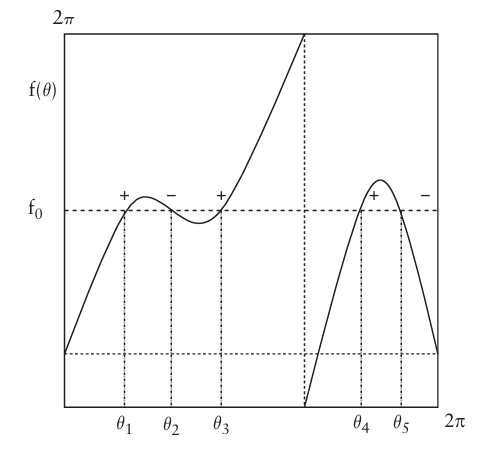
\includegraphics[scale = 0.5]{Screenshot 2026-02-05 110949.png}
    \end{center}

    Prendendo qualsiasi membro del codominio \(f_0\), si può sommare il segno della derivata nei punti in cui \(f(\theta) = f_0\). In questo caso, il grado della mappa è 1, e questo riflette il fatto che la mappa fa un giro completo del cerchio. 

    Data la mappa \(f\), uno può semplicemente calcolare il grado della mappa usando la sua definizione. Scegliendo la forma di volume \(\omega = d\theta\), allora si ottiene 

    \begin{align}
        N = \frac{1}{2\pi}\int_{S^1} f^*d\theta = \frac{1}{2\pi}\int_0^{2\pi}\left(\frac{df}{d\theta} \right)d\theta
    \end{align}
}

\ex{Altre formule utili}{

    Possiamo formulare un simile argomento per calcolare il grado di una funzione \(f: S^2 \rightarrow S^2\). Indicando con \(x^i\) le coordinate locali sulla 2-sfera di partenza, avremo \(f^a(x^i) \in \mathbb{R}^3\), t.c. \(|f|=1\). Per calcolare il grado di questa funzione, scegliamo la forma di volume standard sulla due sfera, ovvero 
    
    \begin{align}
        \omega = \frac{1}{2}\eps_{abc} x^a dx^b \wedge dx^c
    \end{align}

    Il pullback sullo spazio di base attraverso la funzione \(f\) è dato esplicitamente allora da 

    \begin{align}
        f^*\omega = \frac{1}{2}\eps_{abc}f^a df^b \wedge df^c = \frac{1}{2}\eps_{abc}f^a \frac{\partial f^b}{\partial x^i}\frac{\partial f^c}{\partial x^j}dx^i \wedge dx^j = \frac{1}{2}\eps_{abc}\eps^{ij}f^a \frac{\partial f^b}{\partial x^i}\frac{\partial f^c}{\partial x^j}d^2x  
    \end{align}

    concludiamo che il grado è dato dalla formula 

    \begin{align}
        \deg{(f)} = \frac{1}{8\pi}\int_{S^2} \frac{1}{2}\eps_{abc}\eps^{ij}f^a \frac{\partial f^b}{\partial x^i}\frac{\partial f^c}{\partial x^j}d^2x 
    \end{align}

    Con gli stessi passaggi, si ottiene la formula per \(X \rightarrow S^3\) (in particolare usando la forma di volume standard su \(S^3\), che è data da \(\omega = (1/3!)\eps_{abcd}x^a dx^b \wedge dx^c \wedge dx^d\))

    \begin{align}
        \deg(f) = \frac{1}{12\pi^2}\int_X \eps_{abcd}\eps^{ijk}f^a (\partial_i f^b)(\partial_j f^c)(\partial_k f^d)
    \end{align}

    Equivalentemente, sfruttando l'isomorfismo \(S^3 = SU(2)\), possiamo pensare che \(f\) abbia valori nel gruppo. Allora si motra che vale la relazione 
    
    \begin{align}
        \deg(f) = \frac{1}{(24\pi^2)}\int_X \text{Tr}[(f^{-1}df)^3]
    \end{align}

}

\subsection{Omotopia}

Consideriamo una funzione \(f\), \emph{liscia}, a valori da \(M\) in \(N\). \\

Una omotopa ad \(f\) è una mappa anch'essa liscia, 

\begin{align}
    F: M \times [0, 1] \rightarrow N, \, : \, F[x, 0] = f(x)
\end{align}

In particolare, ogni funzione \(f_t(x):= F[x, t]\), si dice essere \emph{omotopica} ad \(f\). Dunque, l'omotopia è una classe di equivalenza, e le mappe lisce possono essere \emph{classificate}, in base alla classe di omotopia. \\

Indichiamo con \(\pi_1(M, x_0)\) l'insieme delle classi di omotopia dei loop. Si tratta delle funzioni \(f: [0,1] \rightarrow M\), t.c. \(f(0) = f(1) = x_0\). In pratica, si tratta delle curve chiuse in \(M\). 

Questo spazio ha la struttura di un gruppo, nel senso che è possibile definire una operazione di moltiplicazione fra loops, che rispetta le regole di un gruppo. In particolare \(f_1 * f_2\) è dato dal percorrere prima il loop 1, poi il loop 2. In formule, avremmo 

\begin{align}
    (f_1 * f_2)(t) = \begin{cases}
        f_1 (2t), \, t \in [0, 1/2] \\ f_2(2t-1), \, t \in [1/2, 1] 
    \end{cases} 
\end{align}

L'inversa di un loop è data semplicemente da \(\hat{f} = f(1-t)\). Il gruppo \(\pi_1(M)\) è detto \emph{gruppo fondamentale}, ed in particolare definiamo \(M\) semplicemente connesso, se il gruppo fondamentale è banale. 

\ex{\(\pi_1(S^1)\)}{

    Studiamo per esercizio il set delle classi di omotopia dei loop a valori sulla \(S^1\). In particolare, la condizione di chiusura del loop implica che deve valere 

    \begin{align}
        f(0) = 0, \quad f(1) = 2\pi k, \quad k \in \mathbb{Z}
    \end{align}

    In particolare, tutte le mappe con lo stesso \(k\) sono omotopiche. Questo può essere verificato dalla funzione

    \begin{align}
        f_\tau = (1-\tau)f_1 + f_2
    \end{align}

    con \( f_1, f_2\) aventi lo stesso \(k\). 

    Concludiamo che \(\pi_1(S^1) = \mathbb{Z}\)

}

I set \(\pi_k(M)\) generalizzano \(\pi_1(M)\), nel senso che si tratta delle classi di equivalenza delle mappe \([0, 1]^k \rightarrow M\), tali che mandino il bordo di \([0, 1]^k\) in un punto \(\in M\). La struttura del gruppo è preservata estendendo la definizione di moltiplicazione a 

\begin{align}
    (f_1 * f_2)(t_1, \ldots, t_k) = \begin{cases}
        f_1(t_1, \ldots, t_{k-1}, 2t_k), \, t_k \in [0, 1/2] \\
        f_1(t_1, \ldots, t_{k-1}, 2t_k - 1), \, t_k \in [1/2, 1]
    \end{cases} 
\end{align}


In particolare, il gruppo è abeliano per \(k>1\). \\

Quando abbiamo parlato del grado di una mappa, abbiamo dato una formula per calcolarlo, nel in cui questa fosse una mappa \emph{liscia}. Se invece la mappa è continua? In questo caso, esiste sempre una mappa liscia, a cui quella continua è omotipica. Definiamo dunque il grado della mappa continua come il grado di questa mappa liscia. Conseguenza di questa definizione è che due mappe sono omotopiche se e solo se hanno lo stesso grado: dunque, calcolare il grado di una mappa è un buon modo per calcolare la classe di omotopia di una mappa. 













































\section{Le teorie dei campi classiche}

Consideriamo uno spaziotempo di Minkowski \((1+D)\)-dimensionale, con segnatura \((+, -, ..., -)\). Indicheremo le coordinate su questo spazio con \(x^{\mu} = (t, \vec{x})\), con \(t \in \mathbb{R}\), \(\vec{x}\in \mathbb{R}^{D}\). Questo vuol dire che scriveremo 

\begin{align}
    ds^2 = h_{\mu\nu}dx^{\mu}dx^{\nu} = dt^2 - (d\vec{x}^2)
\end{align}

Come si fa una teoria di \(N\) campi scalari relativistica su questo spazio? \\ 

Inanzitutto, consideriamo la funzione \(\phi : \mathbb{R}^{1+D} \rightarrow Y \subset \mathbb{R}^N\), di cui indicheremo le componenti con \(\phi^a, \, a = 1, .., N\). Tali funzioni sono dette campi, perchè sono funzioni delle coordinate dello spaziotempo. \\

A partire da queste, supponiamo di costruire una densità lagrangiana, che supponiamo essere funzione dei campi, e delle loro derivate. Scriveremo dunque 

\begin{align}
    \mathcal{L} = \mathcal{L}(\phi^a, \partial_\mu \phi^a)
\end{align}

Tale scelta deriva dal fatto di voler scrivere delle equazioni di grado al massimo secondo. In alcune applicazioni esotiche, le equazioni differenziali possono essere di grado superiore al secondo, e si prendono lagrangiane che dipendono dalle derivate dei campi fino all'ordine \(m\). Noi ci limiteremo a prendere \(m = 2\). \\

Ora, le equazioni del moto dei campi si scrivono prendendo il principio di minima azione, ovvero la configurazione dei campi nello spaziotempo, sarà quella che minimizzerà il funzionale 

\begin{align}
    S = \int_{\mathbb{R}\times \mathbb{R}^D}\mathcal{L}dx^{D}dx
\end{align}

Abbiamo già mostrato che questo porta a delle equazioni del moto della forma 

\begin{equation}
    \frac{\partial \mathcal{L}}{\partial \phi^a} - \partial_\mu \frac{\partial \mathcal{L}}{\partial (\partial_\mu \phi^a)} = 0 
\end{equation}

Tra le tante proprietà interessanti di queste equazioni, sottoliniamo che sono le stesse se considero invece una lagrangiana 

\begin{align}
    \mathcal{L}' = \mathcal{L} + \eps \partial_\mu B^{\mu}
\end{align}

Dunque, se l'azione di un gruppo \(G\) sui campi \(\phi^a\) (e sulle loro derivate), modifica la lagrangiana aggiungendo semplicemente una derivata totale, questo non cambia le equazioni del moto, e possiamo pensare che il gruppo \(G\) realizzi una simmetria per il sistema. \\

Facciamo dunque l'ipotesi che un gruppo \(G\) agisca in questo modo sulla nostra lagrangiana. In generale, un gruppo \(G\) agisce sui campi con una legge di trasformazione che sarà data (in un opportuno intorno dell'identità), da 

\begin{align}
    \phi'^a = \phi^a + \eps W^a
\end{align}

Che a sua volta implica che le derivate si trasformano come 

\begin{align}
    \partial_\mu \phi'^a = \partial_\mu \phi^a + \eps \partial_\mu W^a
\end{align}

da cui deduciamo come si trasforma la lagrangiana:

\begin{align}
    \mathcal{L}' &= \mathcal{L} + \eps\left[\frac{\partial \mathcal{L}}{\partial \phi^a} W^a + \frac{\partial \mathcal{L}}{\partial (\partial_\mu \phi^a)}\partial_\mu W^a\right] \\
    &= \mathcal{L} + \eps\partial_\mu\left[\frac{\partial \mathcal{L}}{\partial (\partial_\mu \phi^a)}W^a\right] +\eps W^a \left[\frac{\partial \mathcal{L}}{\partial \phi^a} - \partial_\mu \frac{\partial \mathcal{L}}{\partial (\partial_\mu \phi^a)}\right] \\
    &= \mathcal{L} + \eps\partial_\mu\left[\frac{\partial \mathcal{L}}{\partial (\partial_\mu \phi^a)}W^a\right] = \mathcal{L} + \eps \partial_\mu B^{\mu}
\end{align}

Abbiamo dunque mostrato l'esistenza di un vettore a divergenza nulla: 

\begin{align}
    J^{\mu} := \frac{\partial \mathcal{L}}{\partial (\partial_\mu \phi^a)}W^a - B^\mu
\end{align}

Ciò implica che la \emph{carica di Noether}
\begin{align}
    Q := \int_{\mathbb{R}^D}J^0 dx^D 
\end{align}

è costante nel tempo, a patto che la componente temporale si annulli all'infinito. Infatti, vale 

\begin{align}
    \frac{dQ}{dt} &= \int_{\mathbb{R}^D} \frac{\partial J^0}{\partial t} dx^D \\
    &= -\int_{\mathbb{R}^D} \vec{\nabla}\cdot \vec{J} = \Phi_S(\vec{J})
\end{align}


\ex{Lagrangiana naturale}{
    Consideriamo una lagrangiana del tipo 
    \begin{align}
        \mathcal{L} = \frac{1}{2}\partial^\mu \phi^a\partial_\mu\phi^a - U(\phi) 
    \end{align}

    Che equazioni del moto sono associate a questa lagrangiana? Possiamo effettuare il calcolo. In particolare, calcoliamo 

    \begin{align}
        \frac{\partial \mathcal{L}}{\partial \phi^a} = - \frac{\partial U}{\partial \phi^a}
    \end{align}
    \begin{align}
        \frac{\partial \mathcal{L}}{\partial (\partial_\mu \phi^a)} &= \frac{\partial}{\partial (\partial_\mu \phi^a)} \left(\frac{1}{2}\partial^\nu \phi^b\partial_\nu\phi^b\right) = \frac{1}{2}\left[\delta^{\mu\nu}\delta^b_a \partial_\nu \phi^b + \partial^\nu \phi^b \delta_\nu^\mu \delta^b_a\right] \\
        &= \frac{1}{2}\left[\partial^\mu \phi^a + \partial^\mu \phi^a\right] = \partial^\mu \phi^a
    \end{align}

    Dunque le equazioni sono date da 
    \begin{align}
        \frac{\partial U}{\partial \phi^a} + \partial_\mu\partial^\mu \phi^a = 0 
    \end{align}

    Parliamo ora delle simmetrie di questa lagrangiana: consideriamo una trasformazione generica delle coordinate \(x^\mu \rightarrow x^\mu + \eps V^\mu(x^\nu)\). La variazione dei campi e della lagrangiana sono date dalla derivata di Lie di queste rispetto al campo \(V^\mu\), che indichiamo come \(\text{Lie}_V (\phi / \mathcal{L})\). Un caso particolarmente interessante è se \(V^\mu\) è costante: in questo caso il gruppo \(G\) non è altro che il gruppo delle traslazioni spazio-temporali. Possiamo chiederci quale è la corrente di Noether conservata: 
    Usando la formula che abbiamo trovato, questo equivale a dire che dobbiamo trovare \(W^a, B^\mu\): 

    \begin{enumerate}
        \item \(W^a\): \\
        La trasformazione sulle coordinate 
        \begin{align}
            x^\mu \rightarrow x^\mu + \eps V^\mu
        \end{align}

        Induce una trasformazione sui campi, data da 
        \begin{align}
            \phi^a(x^\mu) \rightarrow \phi^a(x^\mu + \eps V^\mu) = \phi^a (x^\mu) + \eps (\partial_\mu \phi^a) V^\mu
        \end{align}
        Che mostra 
        \begin{align}
            W^a = (\partial_\mu \phi^a)V^\mu
        \end{align}
        \item \(B^\mu\): \\
        Come detto, la variazione della lagrangiana è data dalla sua derivata di lie sotto il flusso di \(V^\mu\). Scriviamo allora 

        \begin{align}
            \mathcal{L} \rightarrow \mathcal{L} + \eps \text{Lie}_V (\mathcal{L}) = \mathcal{L} + \eps (\partial_\mu \mathcal{L})V^{\mu}
        \end{align}
        Che mostra 
        \begin{align}
            B^{\mu} = \mathcal{L}V^{\mu}
        \end{align}
    \end{enumerate}

    Unendo queste informazioni, troviamo una corrente conservata data da 
    \begin{align}
        J^\mu = \frac{\partial \mathcal{L}}{\partial (\partial_\nu \phi^a)}(\partial_\nu \phi^a)V^\mu - \mathcal{L}V^{\mu}
    \end{align}
    D'altra parte, poiché il vettore \(V^\mu\) è costante, in realtà la condizione di divergenza nulla ci dice che 
    \begin{align}
        \partial_\mu \left(\frac{\partial \mathcal{L}}{\partial (\partial_\nu \phi^a)}(\partial_\nu \phi^a) - \mathcal{L}\right) =0
    \end{align}
    Infine, posso moltiplicare per il tensore metrico \(\eta^\mu_\nu\) (che è costante), e trovo un tensore di grado due, che ha divergenza nulla, noto come il \emph{tensore di energia-impulso}: 

    \begin{align}
        T^\mu_\nu = \frac{\partial \mathcal{L}}{\partial (\partial_\mu \phi^a)}(\partial_\nu \phi^a) - \eta^\mu_\nu\mathcal{L}
    \end{align}
    
    A questo punto, uno può chiedersi quali sono le cariche associate a questa corrente, e troviamo che vale

    \begin{align}
        &E = \int_{\mathbb{R}^D}T^0_0 dx^D \\
        &P_i = -\int_{\mathbb{R}^D}T^0_i dx^D 
    \end{align}

    Il che rivela anche il significato del nome del tensore. 
}


\subsection{I solitoni}

Introduciamo ora un concetto molto importante che ci sarà utile quando introdurremo una simmetria di gauge. Diamo la definizione formale: 

\dfn{Solitoni}{
    I solitoni sono soluzioni statiche, non singolari, ed a energia finita delle equazioni di campo classiche. 
}

Si tratta di oggetti importanti perchè dopo la quantizzazione diventano di fatto le particelle (in 3+1 dimensioni). \\
Consideriamo per semplicità uno spazio (1+1)-dimensionale. Consideriamo una lagrangiana naturale, 

\begin{align}
    \mathcal{L} = \frac{1}{2}(\partial_\mu \phi)(\partial^\mu \phi) - V(\phi) = \frac{1}{2}(\phi_t)^2 - \frac{1}{2}(\phi_x)^2 - V(\phi)
\end{align}

Le equazioni del moto sono date da 
\begin{align}
    \phi_{tt} - \phi_{xx} = -\frac{dV}{d\phi}
\end{align}

Per avere un vuoto stabile, scegliamo di prendere deve valere \(V(\phi) \geq V_0\). Senza ledere alla generalità, scegliamo di prendere \(V_0 =0\). \\

Immaginiamo di prendere un potenziale tale che il set \(V^{-1}(0)\) sia discreto e non vuoto (cioè che vi sia un numero finito di minimi isolati). Denotiamo con \(\phi_i\) gli elementi di questo insieme. Questi sono elementi fondamentali, perchè le soluzioni ad energia finita tendono asintoticamente a queste (se no l'energia, che ricordiamo essere l'integrale su tutto l'asse reale di \(\phi_x^2/2 + V(\phi)\), divergerebbe). \\

Il più semplice tipo di solitoni è dato da quelli con condizioni iniziali date da 
\begin{align}
    &\phi \xrightarrow{x \rightarrow -\infty} \phi_1 \\
    &\phi \xrightarrow{x \rightarrow +\infty} \phi_2
\end{align}

e sono detti \emph{solitoni kink}.

Considero allora l'equazione per le soluzioni stazionarie: 
\begin{align}
    \phi_{xx} = \frac{dV}{d\phi}
\end{align}

che è formalmente identica alla equazione di Newton. Si può ridurre alle quadrature prima integrando rispetto a \(\phi\): 

\begin{align}
    \frac{1}{2}\phi_x^2 = V(\phi) + \text{cost.}
\end{align}

Ci rendiamo poi conto che le condizioni al contorno implicano \(\text{cost.} =0\), e possiamo allora scrivere 

\begin{align}
    \frac{\phi_x^2}{2V(\phi)} = 1 \implies \frac{\phi_x}{\sqrt{2V(\phi)}} = \pm 1 \implies \int \frac{d\phi}{\sqrt{2V(\phi)}} = \pm (x-x_0) 
\end{align}

Inoltre, l'energia potenziale di queste soluzioni si calcola facilmente come 
\begin{align}
    U = \int_\mathbb{R} \left(\frac{1}{2}\phi_x^2 + V(\phi) \right)dx = 2 \int_\mathbb{R} V(\phi)dx  
\end{align}

\ex{Calcolo di un solitone kink}{

    Consideriamo un potenziale dato da 
    \begin{align}
        V(\phi) = \lambda^2 \frac{(\phi^2 - a^2)^2}{2}
    \end{align}

    Osserviamo che \(V^{-1}(0) = \left\{\phi_1 = -a, \phi_2 = a\right\} \). Calcoliamo allora 

    \begin{align}
        x -x_0 = \pm \int_0^\phi \frac{d\tilde{\phi}}{\sqrt{2V(\tilde{\phi})}} = \pm \frac{1}{\lambda}\int_0^\phi \frac{1}{\tilde{\phi}^2 - a^2} = \pm \frac{1}{\lambda a}\tanh^{-1}(\phi/a)
    \end{align}

    Che possiamo facilmente invertire per ottenere 
    \begin{align}
        \phi_k(x) = \pm a \tanh(\lambda a (x-x_0))
    \end{align}

    Osserviamo che come ci aspettavamo questa rispetta le condizioni iniziali. \\

    Potremmo anche calcolare l'energia di questa soluzione, data da 

    \begin{align}
        U = 2\int_\mathbb{R} V(\phi_k (x))dx = \frac{(\lambda a^2)^2}{2}\int_{\mathbb{R}} \frac{dx}{\cosh (\lambda a (x-x_0))}
    \end{align}

    Facendo il cambio di variabili \(\xi = \lambda a x\), troviamo che 
    \begin{align}
        U = \frac{\lambda a^3}{2}\int_{\mathbb{R}}\frac{d\xi }{\cosh^4 (\xi)}
    \end{align}

    Mathematica mi ha suggerito la primitiva dell'integranda, data da \(\tanh(\xi) - \tanh(\xi)^3 /3\). Sapendo questo trovo che l'integrale fa \(4/3\), e dunque posso concludere che 

    \begin{align}
        U = \frac{2}{3}\lambda a^3 
    \end{align}

    Di seguito un grafico che mostra \(V(\phi_k), \phi_k(x)\): \\

    \begin{center}
    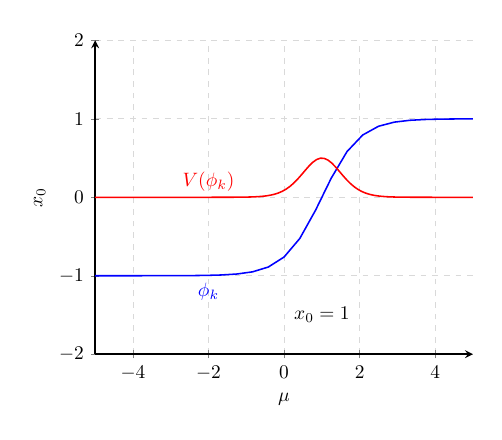
\begin{tikzpicture}[scale=0.7]
        \begin{axis}[
        ymin =-2, ymax=2, 
        xmin=-5, xmax=5, 
        xlabel = {$\mu$},
        ylabel = {$x_0$},
        grid = both,                % griglia
        grid style = {dashed, gray!30},
        axis lines = left,          % assi più puliti
        thick, % linee più spesse
    ]


    \addplot[color=blue]{tanh(x-1)};
    \addplot[color=red, samples = 100]{1/(2*(cosh(x-1))^4)};

    \node at (axis cs:1, -1.5) [color=black]{$x_0=1$};
    \node at (axis cs:-2, -1.2) [color=blue]{$\phi_k$};
    \node at (axis cs:-2, 0.2) [color=red]{$V(\phi_k)$};

    \end{axis}
    \end{tikzpicture}
    \end{center}

    Notiamo in particolare che l'energia del kink è localizzata in \(x_0\). Questo ci permette di identificare il kink come una sorta di particella in \(x_0\), e l'energia \(U\) con la massa della particella. \\

    Infine, notiamo che possiamo ottenere un kink in moto, usando un boost di lorentz su \(\phi_k\): 
    \begin{align}
        \phi(x, t) = \phi_k [\gamma(x-vt)]
    \end{align}
}

Di fatto, la stabilità dei kink è dovuta alla conservazione di cariche topologiche, che sono molto diverse dalle cariche di Noehter, associate ad una simmetria continua della lagrangiana. \\

\subsection{Le equazioni di Bogomolny}

Ora, ci chiediamo tra tutte le configurazioni ad energia finita, quale è la configurazione ad energia più bassa. In effetti, esiste un limite inferiore sull'energia di un kink. Infatti, dato un qualsiasi potenziale finito, esiste sempre una funzione \(W(\phi)\) t.c. 

\begin{align}
    V(\phi) = \frac{1}{2}\left(\frac{dW}{d\phi}\right)^2
\end{align}

D'altra parte, l'energia totale è data da 

\begin{align}
    E &= T + V = \int_{\mathbb{R}}\left(\frac{1}{2}\phi_t^2 + \frac{1}{2}\phi_x^2 + V(\phi)\right)dx \\
    &= \frac{1}{2}\int_\mathbb{R}\left(\phi_t^2 + \phi_x^2 + W_\theta^2\right)dx \\
    &= \frac{1}{2}\int_\mathbb{R}\left(\phi_t^2 + (\phi_x \pm W_\theta)^2 \mp 2W_\theta \phi_x\right)dx \\
    &= \frac{1}{2}\int_\mathbb{R}\left(\phi_t^2 + (\phi_x \pm W_\theta)^2\right) dx \mp \int_{\mathbb{R}} \frac{dW}{dx} dx
\end{align}

Scegliendo il segno meno nella prima somma, possiamo scrivere che 

\begin{align}
    E \geq W(\phi(+\infty)) - W(\phi(-\infty)) = W(\phi_1) - W(\phi_2)
\end{align}

Questo è noto come limite di Bogomolny, e dipende solo dal comportamento asintotico (le condizioni al contorno) del kink. \\

Possiamo dunque dire che le configurazioni statiche con energia minima devono soddisfare \(\phi_t = 0\), devono saturare il limite di Bogomolny, e dunque devono rispettare la cosidetta \emph{equazione di Bogomolny}: 

\begin{align}
    \frac{d\phi}{dx} = \frac{dW}{d\phi}
\end{align}

Tipicamente, questa è più semplice da risolvere rispetto alle equazioni di campo. 

\subsection{L'argomento di Derrick}

Fatta questa discussione, ci chiediamo se e come è possibile generalizzare questi risultati ad uno spazio \(D+1\)-dimensionale. Di fatto, questo è possibile farlo solo per \(D=2\). Derrick mostrò questo usando un semplice argomento di scala: \\

Consideriamo una configurazione \(\phi_1\) tale che sia una soluzione statica delle eq di Eulero-Lagrange, ovvero di 

\begin{align}
    \nabla^2 \phi = \frac{d V}{d\phi}
\end{align}

e che sia un punto critico del funzionale energia, 

\begin{align}
    E[\phi_1] = \int_{\mathbb{R}^D} \left\{\frac{1}{2}|\nabla\phi_1|^2 + V(\phi_1)\right\} = E_{\text{grad}, 1} + E_{V, 1}
\end{align}

Ora, consideriamo la famiglia ad un parametro di campi data da \(\phi_{(c)} = \phi_1(cx)\). Possiamo calcolare il funzionale di energia \(E[\phi_{(c)}]\): 

\begin{align}
    E [\phi_{(c)}] = \int_{\mathbb{R}^D} \left\{\frac{1}{2}|\nabla \phi_1(cx)|^2 + V(\phi_1(cx))\right\}
\end{align}

Facciamo un cambio di variabile di integrazione \(\xi = cx\), ed otteniamo 

\begin{align}
    E[\phi_{(c)}] = \frac{1}{c^D}\int_{\mathbb{R}^D} \left\{\frac{1}{2}|\nabla_x \phi_1(\xi)|^2 + V(\phi_1(\xi))\right\}
\end{align}

Chiaramente vale 

\begin{align}
    \nabla_x = \left(\frac{\partial}{\partial x_1}, \ldots, \frac{\partial}{\partial x_D} \right) = \left(\frac{\partial \xi_j}{\partial x_1}\frac{\partial}{\partial \xi_j}, \ldots, \frac{\partial \xi_j}{\partial x_D}\frac{\partial}{\partial \xi_j} \right) = c \nabla_\xi
\end{align}

Scriviamo allora che 

\begin{align}
    E[\phi_{(c)}] = \frac{1}{c^D}\int_{\mathbb{R}^D} \left\{\frac{c^2}{2}|\nabla_\xi \phi_1(\xi)|^2 + V(\phi_1(\xi))\right\} = \frac{E_{\text{grad}, 1}}{c^{D-2}} + \frac{E_{V,1}}{c^D}
\end{align}

Ora, poiché \(\phi_1\) è un minimo, vale sicuramente che 

\begin{align}
    \frac{dE[\phi_c]}{dc}\biggr|_{c=1} = 0
\end{align}

Facendo un calcolo diretto, otteniamo che questo equivale a scrivere 

\begin{align}
    (D-2)E_{\text{grad}, 1} + DE_{V, 1} = 0 
\end{align}

Interpetiamo il risultato nel seguente modo: 

\begin{enumerate}
    \item \(D=1\): \\
    Come avevamo già trovato, esistono configurazioni statiche ed ad energia finita, e rispettano 
    \begin{align}
        E_{\text{grad}} = E_V
    \end{align}
    \item \(D=2\): \\
    Possono esistere soluzioni statiche ed ad energia finita, a patto che valga 
    \begin{align}
        E_V = 0 
    \end{align}
    \item \(D=3\): \\
    Non vi sono soluzioni statiche ad energia finita. 
\end{enumerate}

Vedremo che questo risultato cessa di valere quando si modifica il funzionale energia, inserendo anche l'energia di un campo di puro gauge. 




\section{La derivata covariante}

Fino ad ora, abbiamo parlato di simmetrie globali della lagrangiana. Consideriamo il caso in cui ho una lagrangiana naturale, data da 
\begin{align}
    \mathcal{L} = \frac{1}{2}(\partial_t \phi)(\partial^t \phi) - V(|\phi|^2)
\end{align}

Ora, in generale, \(\phi : B \rightarrow F\), cioè è una funzione su una certa base, verso una certa fibra. In particolare, devo stare attento allora quando definisco la sua derivata. Infatti, si ha solitamente che 

\begin{align}
    \partial_t \phi = \lim_{\delta t \rightarrow 0}\frac{\phi(t+\delta t) - \phi(t)}{\delta t}
\end{align}

Ma non posso confrontare \(\phi(t+\delta t), \phi(t)\) poiché sono su due spazi vettoriali diversi! Dovrò piuttosto considerare allora 

\begin{align}
    \partial_t \phi = \lim_{\delta t \rightarrow 0}\frac{\phi(t+\delta t) - T(\phi(t))}{\delta t}
\end{align}

dove \(T\) è il trasporto sullo spazio di \(\phi(t+\delta t)\). \\

D'altra parte, la lagrangiana da cui siamo partiti sembrerebbe avere una simmetria di rotazione. Se supponiamo \(\phi \in \mathbb{R}^2 \simeq \mathbb{C}^1\), possiamo dire che dovrebbe essere invariante sotto \(g \in SO(2) \simeq U(1)\). D'altra parte, cosidero cosa succede esplicitamente alle derivate: 

Sia \(\tilde{\phi} = g\phi\), allora troviamo che: 

\begin{align}
    \partial_t(\tilde{\phi}) = \partial_t (g\phi)=  g (\partial_t \phi)
\end{align}

Ovvero la derivata si trasforma come il campo, e non abbiamo nessun problema. \\

\nt{
Questo però è vero solo nel caso in cui \(g\) non sia funzione del tempo. Ma aspetta un attimo: se sto facendo una teoria relativistica, non può valere che \(g\) agisca indipendentemente dal tempo! Ad esempio, non può agire instantaneamente allo stesso modo su tutto il campo, perchè allora vi sarebbe una trasmissione di informazione a velocità infinita. \\
}

Dovremmo allora considerare che, in generale, varrà \(g = g(t)\), e che 

\begin{align}
    \partial_t(\tilde{\phi}) = g(\partial_t\phi) + (\partial_t g)g^{-1}\tilde{\phi}
\end{align}

Questo è un problema, perchè se la lagrangiana è quella che abbiamo definito, allora in pratica la lagrangiana non è invariante sotto il gruppo delle rotazioni! \\

Torniamo al punto di partenza: dobbiamo capire come confrontare un vettore \(\phi\) che vive in \(F_{x_1}\), ed un vettore \(\psi\) che vive in \(F_{x_2}\). Abbiamo detto che dobbiamo considerare \(T \psi = \tilde{\psi} \in F_{x_1}\). Ma come è fatto \(\tilde{\psi}\)? In particolare, avrò una base \(e_{\mu}\) su \(F_{x_1}\), ed una base \(f_\mu\) su \(F_{x_2}\). Ci sarà allora una legge (detta \emph{connessione}), che permette di scrivere \(f_{\mu} = T(e_\mu)\). \\

In generale, la connessione può essere una funzione qualsiasi. Chiaramente il caso più comodo, e che noi considereremo, è il caso di una connessione lineare. In questo caso, si può semplicemente scrivere 

\begin{align}
    f_{\mu} = A^\nu_\mu e_\nu
\end{align}

La connessione modifica la mia derivata (intuitivamente, la variazione del campo non è solamente data dalla variazione del campo, ma anche dal fatto che sto cambiando il sistema di riferimento), in 

\begin{align}
    \partial_\mu \rightarrow \partial_\mu + A_\mu := \nabla_\mu
\end{align}

Questa è nota come \emph{derivata covariante}. Ci chiediamo ora quanto valga \(\nabla_\mu \tilde{\phi}\). Effettuiamo un calcolo diretto: 

\begin{align}
    \nabla_\mu \tilde{\phi} &= (\partial_\mu + A_{\mu})(g\phi) = (\partial_\mu g)\phi + g(\partial_\mu \phi) + A_\mu g\phi \\
    &= (\partial_\mu g)\phi + g(\partial_\mu \phi) + A_\mu g\phi + g A_\mu \phi - g A_\mu \phi \\
    &= g(\nabla_\mu \phi) + (\partial_mu g)g^{-1}\tilde{\phi} + [A_\mu, g]\phi
\end{align}

Sembra che vi sia ancora un problema: la derivata non si trasforma ancora come il campo. 

\nt{Noi nel fare il conto abbiamo assunto che \(A\) non cambi sotto l'azione del gruppo. Questo però non ha nessun senso di avvenire, e potremmo invece supporre che \(A \rightarrow \tilde{A}\), assumere che la derivata si trasformi come il campo, e trovare allora un modo per determinare \(\tilde{A} = \tilde{A}(A)\)}

Supporremo allora che valga 

\begin{align}
    \tilde{\nabla}_\mu \tilde{\phi} = g \nabla_\mu \phi
\end{align}

Questo ci permette di scrivere 
\begin{align}
    (\partial_\mu + \tilde{A}_\mu)(g\phi) &= (\partial_\mu g)\phi + g\partial_\mu \phi + \tilde{A}_\mu g \phi \\
    &= (\partial_\mu g)\phi + g\partial_\mu \phi + \tilde{A}_\mu g \phi + gA_\mu \phi -gA_\mu \phi \\
    &= \underbrace{g \partial_\mu \phi + gA_\mu \phi}_{= g\nabla_\mu\phi} + \underbrace{(\partial_\mu g)\phi + \tilde{A}_\mu g\phi -gA_\mu \phi}_{=0}
\end{align}

Poichè la seconda parte deve essere 0 per qualunque scelta di \(\phi\), possiamo scrivere 

\begin{align}
    \tilde{A}_\mu g = gA_\mu - (\partial_\mu g) \implies \tilde{A}_\mu = gA_\mu g^{-1} - (\partial_\mu g)g^{-1}
\end{align}

Questa legge di trasformazione si trova scritta a volte in maniera diversa, ricordando che vale 
\begin{align}
    \partial_\mu(g^{-1}) = -g^{-1}(\partial_\mu g)g^{-1}
\end{align}
Si ottiene 
\begin{align}
    \tilde{A}_\mu = gA_\mu g^{-1} + g(\partial_\mu g^{-1})
\end{align}

Ora, dal punto di vista matematico tutto questo ha perfettamente senso. Poichè il campo mandava vettori in fibre diverse, abbiamo dovuto introdurre una connessione (che abbiamo supposto essere lineare) ed abbiamo così cambiato la nozione di derivata opportunamente. \\

D'altra parte dal punto di vista fisico è successo qualcosa di molto strano: noi volevamo considerare un semplice campo \(\phi\), magari che descrivesse la densità di una particella, come l'elettrone. Siamo però stati forzati ad introdurre degli altri campi \(A_\mu\) (4 nel caso di uno spaziotempo 3+1 dimensionale). Inoltre, notiamo che poichè la lagrangiana è ora data da 

\begin{align}
    \mathcal{L} = \frac{1}{2}[(\partial_\mu + A_\mu)\phi][(\partial^\mu + A^\mu)\phi] - V(|\phi|^2) 
\end{align}

Che non contiene termini nelle derivate di \(A_\mu\). Questo non va bene, perchè allora le equazioni di Eulero-Lagange non ci daranno delle leggi del moto per questi campi. Dobbiamo allora inserire un termine nelle derivate di \(A_\mu\), che sia anch'esso invariante sotto l'azione del gruppo. \\

La scelta canonica è di prendere 
\begin{align}
    \mathcal{L} = (\nabla_\mu \phi)(\nabla^\mu \phi) - V(|\phi|^2) - \frac{1}{2}\text{Tr}(F^{\mu\nu}F_{\mu\nu})
\end{align}

Ora, ci accorgiamo di un fatto singolare: il campo di gauge sopravvive anche in assenza di materia, dove la lagrangiana si dice diventare di \emph{puro gauge}:

\begin{align}
    \mathcal{L} = -\frac{1}{2}\text{Tr}(F^{\mu\nu}F_{\mu\nu})
\end{align}

Applicando ora le equazioni di Eulero-Lagrange per un campo, otteniamo che la legge del moto dei campi è data semplicemente da 

\begin{align}
    \nabla_\mu F^{\mu\nu} = 0
\end{align}

\section{Monopoli}

\subsection{Una parentesi sulla notazione}

D'ora in poi useremo spesso le forme differenziali. In particolare, diremo che il campo di gauge è dato da 

\begin{align}
    A = A_\mu dx^\mu
\end{align}

con \(A^\mu : x^{\nu} \in \mathbb{R}^{D+1} \rightarrow g\), dove \(g\) è una rappresentazione di un'algebra di Lie, relaviva a qualche gruppo di Lie \(G\). Usiamo gli indici latini \(a, b, ...\) per indicare i generatori delle algebre di Lie.   

Ed il tensore di intensità del campo e la derivata covariante saranno
\begin{align}
    &F = \frac{1}{2}F_{\mu\nu} dx^{\mu} \wedge dx^{\nu} \\
    &D = d + A
\end{align}


dove le componenti del tensore di intensità sono
\begin{align}
    F^{\mu\nu} = \partial^\mu A^\nu - \partial^\nu A^\mu + [A^\mu, A^\nu]
\end{align}

In questo linguaggio, una trasformazione di gauge trasforma i campi come: 

\begin{align}
    &A' = gAg{-1} - dg g^{-1} \\
    &F' = gFg^{-1}
\end{align}

e vale l'identità di bianchi: 
\begin{align}
    DF = 0
\end{align}

Introduciamo anche la stella di Hodge, l'applicazione lineare dallo spazio delle p-forme \((\Lambda^p)\), nello spazio delle (d+1-p)-forme \((\Lambda^{(d+1-p)})\), definita da 
\begin{align}
    *(dx^{\mu_1} \wedge \cdots \wedge dx^{\mu_p})
= \frac{\sqrt{|\det(\eta)|}}{(D+1-p)!}\,
\varepsilon^{\mu_1 \cdots \mu_p}{}_{\mu_{p+1} \cdots \mu_{D+1}}\,
dx^{\mu_{p+1}} \wedge \cdots \wedge dx^{\mu_{D+1}}
\end{align}

Nel caso di uno spazio di Minkowski 3+1-dimensionale, la stella di Hogde realizza un automorfismo fra le 2-forme, ed in particolare si definisce il tensore duale al tensore di intensità del campo, 

\begin{align}
    (*F)_{\mu\nu} = (1/2)\eps_{\mu\nu\sigma\lambda}F^{\sigma\lambda}
\end{align}

Diremo che il tensore di intensità di campo è self-dual (SD) se vale \(*F = F\), oppure antiself-dual (ASD), se vale \(*F = -F\). \\

\ex{L'azione di Yang-Mills}{

    In termini di forme differenziali, l'azione per una teoria di puro gauge, è data dall'azione di Yang-Mills: 

    \begin{align}
        S_{YM} = -\frac{1}{2}\int_{\mathbb{R}^4}\text{Tr}(F\wedge *F)
    \end{align}

    Per capire perchè questo è il caso, effettuiamo un calcolo istruttivo, per prendere confidenza con la notazione. Il nostro obbiettivo è ottenere che questa è semplicemente l'azione derivata precedentemente, ovvero \(-(1/2)\text{Tr}(F^{\mu\nu}F_{\mu\nu})\). 

    Vale certamente 
    \begin{align}
        F \wedge *F &= \frac{1}{4}F_{\mu\nu}F_{\sigma\lambda} dx^{\mu} \wedge dx^{\nu} \wedge *(dx^{\sigma} \wedge dx^{\lambda}) \\
        &= \frac{1}{8}F_{\mu\nu}F_{\sigma\lambda} \eps^{\sigma\lambda}_{\quad \alpha\beta}(dx^{\mu}\wedge dx^{\nu}\wedge dx^{\alpha}\wedge dx^{\beta})
    \end{align}

    Ci ricordiamo ora che vale l'identità
    \begin{align}
        -(dx^\mu \wedge dx^\nu \wedge dx^\alpha \wedge dx^\beta) = \eps^{\mu\nu\alpha\beta}d^4x
    \end{align}

    Troviamo allora che 
    \begin{align}
        F \wedge *F = -\frac{1}{8}F_{\mu\nu}F_{\sigma\lambda}\eps^{\sigma\lambda}_{\quad \alpha\beta}\eps^{\mu\nu\alpha\beta} d^4x
    \end{align}

    Ora, per capire come trattare il prodotto dei due levi-civita, ci ricordiamo della fondamentale identità

    \begin{align}
        \eps^{\mu\nu\alpha\beta}\eps_{\rho\gamma\alpha\beta} = -2(\delta^\mu_\rho \delta^\nu_\gamma - \delta^\mu_\gamma \delta^\nu_\rho)
    \end{align}

    Ed alziamo due indici con il tensore metrico: 
    \begin{align}
        \eps^{\mu\nu\alpha\beta}\eps^{\sigma\lambda}_{\quad \alpha\beta} &= \eps^{\mu\nu\alpha\beta}\eps_{\rho\gamma\alpha\beta}\eta^{\rho\sigma}\eta^{\gamma\lambda} \\
        &= -2(\eta^{\mu\sigma}\eta^{\nu\lambda} - \eta^{\mu\lambda}\eta^{\nu\sigma})
    \end{align}

    Sostituendo quello che abbiamo trovato, 
    \begin{align}
        F \wedge *F &= \frac{1}{4}F_{\mu\nu}F_{\sigma\lambda}(\eta^{\mu\sigma}\eta^{\nu\lambda} - \eta^{\mu\lambda}\eta^{\nu\sigma})d^4x \\
        &= \frac{1}{4}[F_{\mu\nu}F^{\mu\nu}-F_{\mu\nu}F^{\nu\mu}]d^4x \\
        &= \frac{1}{2}F_{\mu\nu}F^{\mu\nu}d^4x
    \end{align}

    Dunque abbiamo scoperto che 
    \begin{align}
        S_{YM} = -\frac{1}{2}\int_{\mathbb{R}^4}\text{Tr}(F\wedge *F) = -\frac{1}{4}\int_{\mathbb{R}^4}\text{Tr}(F_{\mu\nu}F^{\mu\nu})d^4x
    \end{align}
}

\subsection{L'argomento di Derrick pt. 2}

L'argomento di Derrick nel caso di una teoria di gauge porta a diverse conclusioni, perchè il funzionale dell'energia ora tiene conto anche dell'energia del campo di puro gauge. \\

Supponiamo allora che \(\phi_1, A_1\) siano un minimo di 

\begin{align}
    E[\phi, A] = \int_{\mathbb{R}^D}\left\{|F|^2 + |D\phi|^2 + V(\phi)\right\}d^Dx = E_{F} + E_{D\phi} + E_V
\end{align}

Considero allora le famiglie di campi 

\begin{align}
    \phi_c = \phi_1 (cx), \quad A_c = cA_1 (cx) \implies D\phi_c = cD\phi_1 (cx), \quad F_c = c^2 F(cx)  
\end{align}

Possiamo scrivere quando vale l'energia per questa famiglia: 

\begin{align}
    E[\phi_c, A_c] = \frac{E_F}{c^{D-4}} + \frac{E_{D\phi}}{E^{D-2}} + \frac{E_V}{c^D}
\end{align}

Imponendo poi che la derivata rispetto a \(c\) si annulli in \(c=1\), otteniamo che deve valere

\begin{align}
    (D-4)E_F + (D-2)E_{D\phi} + DE_V = 0
\end{align}

\nt{Con l'aggiunta del campo di puro gauge, l'argomento di Derrick non esclude che possano esistere solitoni in \(D = 3, 4\). In realtà l'argomento non ne prova l'esistenza, prova solamente che sicuramente non esistono per \(D > 4\). In ogni caso, si può dimostrare che esistono solitoni per 3 e 4 dimensioni, ed in particolare nello spazio di Minkowski 3+1 dimensionale devono soddisfare 
    \begin{align}
        E_F = E_{D\phi}
    \end{align}
    Questo tipo di solitoni sono detti \emph{monopoli non-abeliani}, per ragioni che diverranno più chiare in seguito. 
}

\subsection{I monopoli di Dirac}

Cominciamo considerando l'elettromagnetismo classico: questa è una teoria classica di gauge, con gruppo di gauge \(U(1)\), sullo spaziotempo di Minkowski 3+1-dimensionale. \\

L'intensità del campo è data da 

\begin{align}
    F = E_idx^i + \frac{1}{2}\eps_{ijk}B^i dx^j \wedge dx^k
\end{align}

Data una corrente \(j_\mu\), si definisce la 1-forma \(J = j_\mu dx^mu\), e le equazioni di Maxwell sono date da 

\begin{align}
    &d F = 0 \\
    &d * F = *J 
\end{align}

Si ricordi che \(*F \in \Lambda^2\), così che \(d * F \in \Lambda^3\), ed inoltre \(J \in \Lambda^1 \implies *J \in \Lambda^3\). \\

Ora, lo spazio di Minkowski è uno spazio semplicemente connesso. In particolare dunque, l'equazione \(dF =0\), implica non solo la chiusura ma anche l'esattezza di F, che infatti si può scrivere come \(dA\). D'altra parte, questo sembrerebbe mostrare che non esistono monopoli magnetici, perchè il flusso del campo magnetico uscente da una sfera è sempre zero. \\

D'altra parte, sappiamo che se ci mettiamo in uno spazio che non è più semplicemente connesso, allora l'argomento precedente viene smontato: prendiamo infatti \(\mathbb{R}^3 \left\{0\right\}\). Topologicamente, qusto spazio è come \(S^2 \times \mathbb{R}\). Come la 2-sfera, dunque, bisogna usare più di una carta per descrivere l'intero spazio. Prendiamo allora due carte, \(U_{\pm}\), che rispettivamente coprano lo spazio \(z > -\eps\), \(z < \eps\). In particolare, le due carte si sovrappongono nella regione \(z \in (-\eps, +\eps)\). \\

Considero ora i potenziali di gauge \emph{regolari} su questi carte, dati da 

\begin{align}
    A_{\pm} = \frac{g}{4\pi}(\pm 1 -\cos\theta)d\phi 
\end{align}

\nt{Questa scelta dei potenziali va bene perchè sono regolari sulle carte, ed in particolare i due sono legati da una trasformazione di gauge:
    \begin{align}
        A_+ = A_- + \frac{g}{2\pi}d\phi
    \end{align}

    Dalla legge di trasformazione è immediato che danno gli stessi campi, poiché \(F = dA\), e vale \(d \left(\frac{g\theta}{2\pi} d\phi\right)=0\). 
}

Ora possiamo semplicemente calcolare i campi: nelle regioni \(U_{\pm}\), varrà \(F = dA\), ovvero 

\begin{align}
    F &= dA = d\left(\frac{g}{4\pi}(\pm1 -\cos\theta) d\phi\right) \\
    &= d\left(\frac{g}{4\pi}(\pm1 -\cos\theta) \right) \wedge d\phi +  \left(\frac{g}{4\pi}(\pm1 -\cos\theta) \right)d^2\phi \\
    &= -\frac{g}{4\pi}\sin(\theta) \, d\theta \wedge d\phi 
\end{align}

è conveniente scrivere il risultato in coordinate cartesiane, e si ottiene 

\begin{align}
    F = \frac{g}{4\pi r^3}\left(xdy\wedge dz + ydz \wedge dx + z dx \wedge dy \right)
\end{align}

Che confrontata con \(F = E_idx^i + \frac{1}{2}\eps_{ijk}B^i dx^j \wedge dx^k\), ci dice immediatamente che i campi sono dati da 

\begin{align}
    \vec{E} = 0,  \quad  \vec{B} = \frac{g \vec{r}}{4\pi r^3}
\end{align}

Interpretiamo dunque il nostro risultato come il campo risultante da un \emph{monopolo magnetico}. In effetti, possiamo calcolare a questo punto il flusso uscente da \(S^2\), ed ottenere 

\begin{align}
    Q &= \int_{S^2} F = \int_{U_+}dA_{+} + \int_{U_{-}}dA_{-} = \int_C (A_+ - A_-) \\
    &= \int_C \frac{g}{2\pi}d\phi = \frac{g}{2\pi}\int_C d\phi
\end{align}

Solo questo sarebbe un risultato notevole. Ma c'è di più: vediamo cosa succede cosa succede quando consideriamo come si accoppia il campo di gauge ai campi di materia: \\

in meccanica quantistica, la derivata covariante si scrive

\begin{align}
    D\psi = (d-iqA)\psi
\end{align}

dove \(q\) è la carica della particella. Ora, in questo caso abbiamo un campo \(\psi_+\) definito nella regione coperta da \(U_+\), che è legato al campo \(\psi_-\) nella regione coperta da \(U_-\) mediante una trasformazione di gauge: in particolare, vale che 

\begin{align}
    \psi_+ = \exp\left(\frac{iqg\theta}{2\pi}\right) \psi_-
\end{align}

Ora, la sua derivata covariante si trasforerà come il campo stesso: 

\begin{align}
    D\psi_+ = \exp\left(\frac{iqg\theta}{2\pi}\right) D\psi_-
\end{align}

D'altra parte, questa deve essere una funzione periodica di \(\phi\), altrimenti non ha senso! Perché ciò valga, deve valere la \emph{condizione di quantizazzione di Dirac}: 

\begin{align}
    qg = 2\pi N, \quad N \in \mathbb{N}
\end{align}

Se in tutto l'universo esistesse un unico monopolo magnetico, allora tutte le cariche dovrebbero essere dei multipli di \(2\pi /g\): in poche parole, capiremmo perchè la carica elettrica è quantizzata. 

\subsection{La fibrazione di Hopf}

Da un punto di vista della geometria differenziale, il numero di monopolo \(N\) classifica i fibrati principali \(U(1)\) su base \(S^2\). \\

Inanzitutto, osserviamo che \(S^2\) è omotopicamente equivalente a \(\mathbb{R}^3 \setminus \left\{0\right\}\). Infatti, consideriamo una mappa \(j: S^2 \rightarrow \mathbb{R}^3\), e \(p: \mathbb{R}^3 \setminus \left\{0\right\} \rightarrow S^2\) la proiezione \(\vec{x} \rightarrow \vec{x}/x\). 

Si ha allora che \(j * p\) è omotopica alla mappa identità attraverso 

\begin{align}
    f(\vec{x}, t) = t\vec{x} - \frac{(1-t)\vec{x}}{x}
\end{align}


Ora, le funzioni di transizione sul fibrato \(U(1)\) sono mappe da \(S^1 \times \mathbb{R}\) ad \(S^1 \times \mathbb{R}\), e sono classificate in base al grado di queste mappe ristrette ad \(S^1\). Nel caso di \(U(1)\), la forma connessione è data da 

\begin{align}
    \omega = \begin{cases}
        A_+ + d\psi_+ \, U_+ \\
        A_- + d\psi_- \, U_-
    \end{cases}
\end{align}

E le funzioni di transizione sono date da \(e^{i\psi_-} = ge^{i\psi_+}\), con \(g \in U(1)\). D'altra parte, per avere un fibrato che è una varietà, le funzioni di transizione devono essere della forma \(e^{iN\phi}\), con \(N \in \mathbb{Z}\). In generale, questa scelta porta ad un fibrato che ha il primo numero di Chern pari a 

\begin{align}
    c_1 = -\frac{1}{2\pi}\int_{S^2}F
\end{align}

Questo numero dipende solamente dalle funzioni di transizione. \\

Dunque la scelta di \(N\) diversi porta a fibrati diversi. Il caso \(N=0\) è il caso dove tutte le mappe di transizione sono l'identità, e dunque è il caso del fibrato triviale \(S^2 \times S^1\). Il caso \(N=-1\) è più interessante, ed è detto \emph{fibrato di Hopf}. Lo spazio del fibrato è dato da \(P= S^3 \subset \mathbb{C}^2\), dunque ne daremo una descrizione in termini di numeri complessi. \\

Consideriamo allora \(Z_0, Z_1 \in \mathbb{C}^2\), la \(S^3\) è allora data esplicitamente da 

\begin{align}
    Z^0 \bar{Z^0} + Z^1\bar{Z^1} = 1
\end{align}

Ora, consideriamo una "linea complessa" \(A_0 Z^0 + A_1 Z^1 = 0\) che passi attraverso l'origine in \(\mathbb{C}^2\). Questa intercetta la 3 sfera in un cerchio \(S^1\) Ora, l'intersezione non dipende liberamente da \(A_0, A_1\), ma piuttosto dal loro rapporto, \(A_1/A_0\). Lo spazio di questi rapporti è diffeomorfo ad \(S^2\). Quindi possiamo pensare che la proiezione dal fibrato allo spazio base sia esplicitamente dato da 

\begin{align}
    \pi: S^3 \rightarrow S^2 \quad (Z^0, Z^1) \rightarrow \frac{Z^1}{Z^0}
\end{align}


Ora occupiamoci di mostrare che \(P(N=-1) = S^3\). Assumeremo che \(P=S^3\), e mostreremo che deve valere \(N=-1\). Per prima cosa, prendiamo una parametrizzazione della \(S^3\). Una possibile scelta è data da

\begin{align}
    Z^0 = \cos (\theta/2)e^{i\xi_0}, \quad Z^1 = \sin(\theta/2)e^{i\xi_1}
\end{align}

con \((\xi_0, \xi_1, \theta) \in \mathbb{R}^2 \times S^1\). Si verifica immediatamente che questo rispetta la condizione \(Z^0\bar{Z}^0 + Z^1 \bar{Z}^1=1\). In terini di questa parametrizzazione, la coordinata proiettata sulla \(S^2\) è data ad 


\begin{align}
    \lambda(\theta, \phi) = \frac{Z^1}{Z^0} = \tan(\theta/2)e^{i\phi}
\end{align}

Ora, poiché \(\theta \in (0, \pi)\) e \(e^{i\phi}\) è una funzione periodica di periodo \(2\pi\), possiamo interpretare la coppia \(\theta, \phi\) come le coordinate sferiche standard della \(S^2\). La metrica sarà allora data da 

\begin{align}
    ds^2 ? d\theta^2  + \sin^2\theta d\phi^2 
\end{align}

Che volgiamo scrivere in termini di \(\lambda, \bar{\lambda}\). Calcoliamo allora 

\begin{align}
    &d\lambda = \left(\frac{1}{2}\sec^2(\theta/2)d\theta + i\tan (\theta/2)d\phi \right)e^{i\phi} \\
    &d\bar{\lambda} = \left(\frac{1}{2}\sec^2(\theta/2)d\theta - i\tan (\theta/2)d\phi \right)e^{-i\phi}
\end{align}

Poichè la metrica deve essere reale, scriviamo 

\begin{align}
    d\lambda d\bar{\lambda} = |d\lambda|^2 = \frac{1}{4}\sec^4 (\theta/2)d\theta^2 + \tan^2(\theta/2)d\phi^2
\end{align}

ora, vale che \(|\lambda|^2 = \tan^2(\theta/2)\), così come \((1+|\lambda|^2) = \sec^2(\theta/2)\). Per riottenere la metrica classica sulla 2-sfera, divido per la secante alla quarta: 

\begin{align}
    \frac{4|d\lambda|^2}{(1+|\lambda|^2)} = d\theta^2 + 4\tan^2(\theta/2)\cos^4(\theta/2)d\phi^2
\end{align}

Con semplice trigonomentria si ottiene che 

\begin{align}
    4\tan^2(\theta/2)\cos^4(\theta/2) = 4\sin^2(\theta/2)\cos^2(\theta/2) = (1-\cos^2\theta) = \sin^2\theta
\end{align}

Così che la metrica sulla \(S^2\) in termini di \(\lambda\) sarà semplicemente data da

\begin{align}
    ds^2 = \frac{4|d\lambda|^2}{(1+|\lambda|^2)^2}
\end{align}

Ora che abbiamo imparato a legare le coordinate \(\lambda\) alle coordinate sferiche, possiamo scrivere esplicitamente la proiezione \(\pi: S^3 \rightarrow S^2\): 

\begin{align}
    \pi(\theta, \phi) = (\sin\theta \cos\phi, \sin\theta \sin \phi, cos\theta) = \left(\frac{\lambda +\bar{\lambda}}{1+|\lambda|^2}, \, \frac{\lambda - \bar{\lambda}}{i(1+|\lambda|^2)}, \, \frac{-1 + |\lambda|^2}{1+|\lambda|^2} \right)
\end{align}

Ora, se vogliamo leggere le funzioni di transizione, dobbiamo vedere come si comporta la fibra in una regione dove due carte si sovrappongono. Notiamo che la proiezione \(Z^1/Z^0\) è valida solo in una carta dove \(Z^0 \neq 0\). D'altra parte, se vale \(Z^0 = 0 \implies Z^1 \neq 0\), e possiamo scrivere che la proiezione su questa carta è data da \(Z^0/Z^1\). Prendiamo allora due sezioni locali del fibrato, 

\begin{align}
    s(\lambda) = \frac{(1, \lambda)}{\sqrt{1+|\lambda|^2}}, \quad \tilde{s}(\tilde{\lambda}) = \frac{(\tilde{\lambda},1)}{\sqrt{1+|\tilde{\lambda}|^2}}
\end{align}

Osserviamo che sono legati l'uno all'altra nella regione di transizione, dove \(Z^0, Z^1 \neq 0\), da 

\begin{align}
    \tilde{s}(\tilde{\lambda}) = \frac{\tilde{\lambda}(1, \lambda)}{\sqrt{1+|\tilde{\lambda}|^2}} = \left(\frac{\tilde{\lambda}}{|\tilde{\lambda}|} \right)s(\lambda) = e^{-i\phi}s(\lambda)
\end{align}

che mostra che, come promesso, \(N=1\). 

\section{Monopoli non-abeliani}

\subsection{Solitoni con algebra \(SU(2)\)}

Cominciamo ora a considerare una teoria di gauge non-abeliana. In particolare, prendiamo \(G = SU(2)\), e scriviamo la lagrangiana di puro gauge + un campo di Higgs, i.e. un campo \(\Phi : \mathbb{R}^{1+3} \rightarrow SU(2)\), che è data da 

\begin{align}
    \mathcal{L} = -\frac{1}{4}F^a_{\mu\nu}F^{a\mu\nu} + \frac{1}{2}(D_\mu \Phi^a)(D^\mu \Phi^a) - U(\phi^a)
\end{align}

Chiaramente questa lagrangiana è invariante se lo è il potenziale \(U(\Phi)\). Una possibile scelta è prendere 

\begin{align}
    U(\Phi) = \frac{c}{4}(|\Phi|^2 - v^2)^2
\end{align}

con  \(v \in \mathbb{R}^+, \, |\Phi|^2 = \Phi^a\Phi^a\). Siamo interessati ai solitoni di questa teoria, ovvero le sue soluzioni statiche, ad energia finita. Quest'ultima condizione assicura che 

\begin{align}
    |\Phi| \rightarrow v, \quad F_{\mu\nu} \rightarrow 0, \quad D_\mu \Phi \rightarrow 0, \quad \text{se } r \rightarrow +\infty
\end{align}

Ora, le equazioni di Eulero-Lagrange associate a questa lagrangiana si ottengono con la solita formula, e sono date da

\begin{align}
    &D_\mu D^\mu \Phi^a = -c(|\Phi|^2 - v^2)\Phi^a \\
    &(D_\nu F^{\mu\nu})^a = -\eps^{abc}\Phi^bD^\mu \Phi^c
\end{align}

Ora, una soluzione banale è data da 
\begin{align}
    |\Phi| = v, \quad A = 0, \quad D_\mu \Phi^a = 0
\end{align}

che è anche la soluzione di energia minima, perchè il campo non ha gradienti ed è sempre nella configurazione che minimizza l'energia potenziale. D'altra parte, queste condizioni non identificano unicamente un'unico \emph{ground state}. In effetti, dato \(\Phi\) in questo stato, posso sempre agire con un elemento di \(U(1)\) ed ottenere un'altro stato ad energia minima. Diremo allora che questo porta ad una rottura spontanea di simmetria \(SU(2)\rightarrow U(1)\), che porta il potenziale di gauge, ed i campi, ad essere simili al caso abeliano \(U(1)\) dell'elettromagnetismo, a grande \(r\). \\

Si noti inoltre come nell'equazione che contiene le derivate seconde del campo di gauge, compaia, grazie alla presenza del campo di Higgs, un termine omogeneo, che potremmo pensare come la massa del bosone di gauge. In effetti, questo è l'unico modo di fare una teoria di interazioni a corta distanza, con bosoni massivi, perchè le teorie di puro gauge descrivono bosoni a massa nulla, e aggiungere un termine \(m^2 Q(A)\), dove la funzione \(Q(A)\) è quadratica nel potenziale di gauge romperebbe certamente la simmetria di gauge.  

\subsection{Topologia dei monopoli}

Cerchiamo allora delle soluzioni statiche e ad energia finita delle nostre equazioni. Scegliamo un gauge dove \(A_0 = 0\). Questo è comodo perchè data qualsiasi funzione \(f\) a valori nell'algebra di \(SU(2)\), allora vale che se \(f\) non dipende esplicitamente dal tempo \(\implies D_0(f) = 0\). Prendiamo anche il caso in cui \(c=0\), e consideremo il campo di Higgs riscalato \(\hat{\Phi} = \Phi / |\Phi|\), in modo tale da non portarci dietro il \(v\). \\

Poichè asintoticamente \(\hat{\phi} = 1\), vedremo che i solitoni sono simili ai monopoli di Dirac per grande \(r\). Una grossa differenza tra i solitoni in teorie di gauge non abeliane (che da qui in avanti cominceremo a chiamare anche monopoli non-abeliani) è che questi sono dati da due campi \(\Phi, F\), e non solamente \(F\) come nel caso abeliano. \\

In ogni caso vicino all'origine le due situazioni differiscono molto, con il caso non-abeliano che in particolare è regolare all'origine, il che lo rende una configurazione ad energia finita. 

Ora, poichè \(A_0 =0\), e siccome tutti i campi sono per ipotesi statici, le uniche forze del campo sono quelle magnetiche, date esplicitamente da 

\begin{align}
    B_k = \frac{1}{2}\eps_{ijk}F^a_{ij}\hat{\phi}^a
\end{align}

Se vogliamo conoscere la carica di questo campo magnetico, dobbiamo calcolarne il flusso. Per farlo, per prima cosa determiniamo \(A^a_i\) e le sue derivate \(F^a_{\mu\nu}\). 

\begin{enumerate}
    \item \(A^a_i\): \\
    Il campo è fissato dal fatto che asintoticamente deve valere \(D_i \hat{\Phi}^a = 0\). Questo implica che 

    \begin{align}
        \partial_i \hat{\Phi}^a + \eps^{abc}A^b_i \hat{\Phi}^c = 0 
    \end{align}

    che è una equazione algebrica per \(A^b_i\). La risolviamo indovinando la soluzione. Prendiamo ad esempio

    \begin{align}
        A^b_i = \eps^{bde}(\partial_i \hat{\Phi}^d)\hat{\Phi}^e
    \end{align}

    sostituendo possiamo verificare che questa soddisfa la nostra equazione. 
    \item \(F^a_{\mu\nu}\): \\
    Si tratta solamente di fare derivate usando la formula \(F^a_{ij} = \partial_i A^a_j - \partial_j A^a_i + \eps^{abc}A^b_i A^c_j\). Facendo i calcoli, si ottiene che 

    \begin{align}
        F^a_{ij} = 2\eps^{abc}(\partial_i \hat{\Phi}^b)(\partial_j \hat{\Phi}^c) - (\eps^{pqr}(\partial_i \hat{\Phi}^p)(\partial_j \hat{\Phi}^q)\hat{\Phi}^r)\hat{\Phi}^a
    \end{align}
\end{enumerate}

Possiamo adesso calcolare il flusso che sarà dato da 

\begin{align}
    Q = \int_{S^2_\infty}\frac{1}{2}\eps_{ijk}(F^a_{ij}\hat{\Phi}^a)n_i d^2S 
\end{align}



\section{Istantoni nelle teorie di Yang-Mills}

Cominciamo con una semplice definizione: 

\dfn{Istantoni}{
    Gli istantoni sono soluzioni non singolari delle equazioni di campo classiche, in spazio euclideo, la cui azione è finita. 
}

In particolare, in questa sezione studieremo gli istantoni in una teoria di puro Yang-Mills, senza campi di materia o il campo di Higgs. \\

In particolare, in spazio euclideo significa che prenderemo una metrica \(\eta = (+, +,+,+)\). In effetti da questo deriva il nome istantone, perchè un evento nello spazio euclideo è simultaneamente localizzato nello spazio e nel tempo. Ma perchè siamo interessati a questo spazio, se le teorie di campo relativistiche si fanno solitamente su Minkowski? \\

La ragione deriva dall'approssimazione semiclassica WKB, che fornisce le correzioni al primo ordine in \(\hbar\): questa prevede che l'ampiezza di tunneling sia esponenzialmente smorzata da \(e^{-S/\hbar}\), dove \(S\) è l'azione tra lo stato di partenza e lo stato di arrivo. \\

Ricordiamo che l'azione di Yang-Mills è data da 

\begin{align}
    S_{YM} = -\int_{\mathbb{R}^4}\text{Tr}(F\wedge *F)
\end{align}

e le equazioni del moto sono date da 

\begin{align}
    D * F =0 
\end{align}

La condizione di azione finita implica che deve valere 

\begin{align}
    F_{\mu\nu} = o(r^{-3}), \, r \rightarrow \infty
\end{align}

e prendiamo allora anche
\begin{align}
    A_{\mu} = \partial_\mu g g^{-1} + o(r^{-2})
\end{align}

Osserviamo che non c'è bisogno di specificare \(g(x)\) su tutto \(\mathbb{R}^4\), ma solo al contorno, in pratica solamente \(g : S^3_{\infty} \rightarrow SU(2)\). \\

Si dice che due spazi hanno una metrica conformalmente equivalente, se le due metriche sono legate da una funzione \(\Omega(x)>0\), liscia, tale che 

\begin{align}
    g_{\mu\nu} = \Omega^2(x)\tilde{g}_{\mu\nu}
\end{align}

In particolare, la stella di Hogde passando ad uno spazio a metrica conformalmente equivalente diventa 

\begin{align}
    \tilde{*} \alpha = \Omega^{D-2p} *\alpha, \quad \forall \alpha \in \Lambda^p
\end{align}

Ora, se prendiamo \(D = 4\) (come nel nostro caso), ricordando che il campo \(F\) è una 2-forma, si ha che \(\tilde{*} F = *F\), il che è sufficiente a mostrare che le equazioni di Yang-Mills sono invarianti conformalmente! Se \(A\) è una soluzione per uno spazio, lo è anche per qualunque altro spazio conforme. Ad esempio, è noto che \(\mathbb{R}^4\) è conforme ad \(S^4\). Possiamo allora pensare che una soluzione su \(S^4\) sia proiettata stereograficamente su \(\mathbb{R}^4\). In effetti, Ulhenbeck ha provato anche l'opposto: per ogni soluzione liscia ed ad azione finita \(A\) delle eq. di YM su \(\mathbb{R}^4\), esiste un fibrato su base \(S^4\), che proietta stereograficamente su \(A\). \\


In particolare, osserviamo che \(S^4\) non è contraibile, e dunque un fibrato principale di \(SU(2)\) con base la 4-sfera può avere una topologia non banale. \\


Sia \(\omega\) una connessione su un fibrato principale \(P\), di base \(S^4\). Denoteremo con \(f_N: S^4 \setminus N \rightarrow \mathbb{R}^4, \, f_S = S^4 \setminus S \rightarrow \mathbb{R}^4\) rispettivamente le proiezioni stereografiche dal polo nord al polo sud. \\ 

Queste proiettano \((d+A_N, \, d+A_S)\) su \(\mathbb{R}^4 \), ma 














\end{document}